\documentclass[11pt]{article}

\usepackage[letterpaper,margin=1in]{geometry}
\usepackage{microtype}
\usepackage{amsmath}
\usepackage{amssymb}
\usepackage[numbers,sort&compress]{natbib}
\usepackage{booktabs}
\usepackage{longtable}   % tab:guidelines outgrew one page at 8 rows
\usepackage{array}
\usepackage{float}
\usepackage{graphicx}
\usepackage{xcolor}
\usepackage{colortbl}
\usepackage[most]{tcolorbox}
\usepackage{enumitem}
\usepackage{caption}
\usepackage[hidelinks]{hyperref}
\usepackage{parskip}
\usepackage[nameinlink,capitalize]{cleveref}
\usepackage[section]{placeins}
\usepackage{titlesec}
\titlespacing*{\section}{0pt}{3.4ex plus .8ex minus .3ex}{1.7ex plus .3ex}
\titlespacing*{\subsection}{0pt}{2.6ex plus .6ex minus .2ex}{1.1ex plus .3ex}
% coloured headings + a running header, so a 70-page report still reads like one document
\definecolor{hdgmaroon}{HTML}{9A2436}
\titleformat{\section}{\normalfont\Large\bfseries\color{hdgmaroon}}{\thesection}{0.6em}{}
\titleformat{\subsection}{\normalfont\large\bfseries\color{hdgmaroon}}{\thesubsection}{0.6em}{}
\titleformat{\subsubsection}{\normalfont\normalsize\bfseries\color{hdgmaroon}}{\thesubsubsection}{0.6em}{}
\usepackage{fancyhdr}
\pagestyle{fancy}\fancyhf{}
\fancyhead[C]{\footnotesize\itshape Benchmark Gains Do Not Guarantee Transfer}
\fancyfoot[C]{\small\thepage}
\renewcommand{\headrulewidth}{0.4pt}
\fancypagestyle{plain}{\fancyhf{}\fancyfoot[C]{\small\thepage}\renewcommand{\headrulewidth}{0pt}}
\setlength{\emergencystretch}{3em}
% A global `\sectionbreak -> \clearpage` used to open every section on a fresh page. On a report
% this long that produced seven near-empty pages, so sections now flow and only the appendix
% boundary is forced (see the \clearpage before \appendix).
% let big floats share a page with text, and pin float-only pages to the top (no centring glue)
\renewcommand{\topfraction}{0.9}
\renewcommand{\bottomfraction}{0.8}
\renewcommand{\textfraction}{0.07}
\renewcommand{\floatpagefraction}{0.85}
\makeatletter\setlength{\@fptop}{0pt}\makeatother
\graphicspath{{figures/}}

% ---- teaching / takeaway callout boxes (reused from the simplified editions) ----
\definecolor{bgblue}{HTML}{EAF2FF}
\definecolor{bgblueedge}{HTML}{2563EB}
\definecolor{tkgreen}{HTML}{EAF7EE}
\definecolor{tkgreenedge}{HTML}{15803D}
\definecolor{guidealt}{HTML}{F2FBF5}   % zebra tint for the guidelines table
\definecolor{guiderule}{HTML}{BFE3CB}  % soft green rule
% ---- executive-spread palette (Evidence/Risk/Action cards + selector diagram) ----
\definecolor{amberfill}{HTML}{FEF3C7}
\definecolor{amberedge}{HTML}{D97706}
\definecolor{cardgrey}{HTML}{F3F4F6}
% tick/cross for the closest-work comparison (tab:closest); amssymb only, no extra font package
\newcommand{\cmark}{\textcolor{tkgreenedge}{\ensuremath{\checkmark}}}
\newcommand{\xmark}{\textcolor{black!45}{\ensuremath{\times}}}
\definecolor{inkgrey}{HTML}{374151}
\usepackage{tikz}
\usetikzlibrary{arrows.meta,positioning,shapes.geometric,fit,backgrounds,matrix}
\newtcolorbox{background}[1]{colback=bgblue,colframe=bgblueedge,title={#1},fonttitle=\bfseries\small,
  fontupper=\small,boxrule=0.5pt,left=4pt,right=4pt,top=3pt,bottom=3pt,breakable}
\newtcolorbox{takeaway}[1]{colback=tkgreen,colframe=tkgreenedge,title={#1},fonttitle=\bfseries\small,
  fontupper=\small,boxrule=0.5pt,left=4pt,right=4pt,top=3pt,bottom=3pt,breakable}
\newcommand{\code}[1]{\texttt{\small #1}}
% ---- worked-example box (Act III case study: a real G0/D1 row a general guard misses) ----
\newtcolorbox{casebox}[1]{colback=amberfill!35,colframe=amberedge,title={#1},
  fonttitle=\bfseries\small,fontupper=\small,boxrule=0.6pt,arc=2pt,
  left=5pt,right=5pt,top=3pt,bottom=3pt}   % non-breakable: the worked example is one unit
% ---- end-of-section result module: Evidence / Decision / Boundary ----
\newtcolorbox{edbox}[1][]{colback=cardgrey,colframe=inkgrey,boxrule=0.7pt,arc=2pt,
  left=5pt,right=5pt,top=3pt,bottom=3pt,fontupper=\small,#1}   % non-breakable: keep E/D/B summary together
\newcommand{\edb}[3]{\begin{edbox}\textbf{\textcolor{tkgreenedge}{Evidence.}}~#1\par\smallskip
  \textbf{\textcolor{bgblueedge}{Decision.}}~#2\par\smallskip
  \textbf{\textcolor{amberedge}{Boundary.}}~#3\end{edbox}}

% ---- study-status banner (reused from Paper B) ----
\definecolor{statusred}{HTML}{9F1239}
\definecolor{statusfill}{HTML}{FFF1F2}
\newcommand{\draftwarning}[1]{%
  \begin{center}
  \fcolorbox{statusred}{statusfill}{%
    \begin{minipage}{0.95\linewidth}\small\textbf{Study status.} #1\end{minipage}}
  \end{center}}


% ---- generated macros bound to the locked results (numbers are never hand-typed) ----
% Auto-generated by analyze_paper_a_sft.py -- do not edit by hand.
\newcommand{\RepDelta}{+0.3234}
\newcommand{\RepCILower}{+0.2647}
\newcommand{\RepCIUpper}{+0.3690}
\newcommand{\RepLCB}{+0.2725}
\newcommand{\TransferDelta}{-0.0589}
\newcommand{\TransferCILower}{-0.0837}
\newcommand{\TransferCIUpper}{-0.0321}
\newcommand{\TransferUCB}{-0.0362}
\newcommand{\TotalSeedCount}{20}
\newcommand{\SpecializationSeedCount}{15}
\newcommand{\UniformGainSeedCount}{5}
\newcommand{\UniformLossSeedCount}{0}
\newcommand{\TransferFavoredSeedCount}{0}
\newcommand{\ZeroAxisSeedCount}{0}
\newcommand{\RepBaseTPR}{0.1296}
\newcommand{\RepSFTTPR}{0.7686}
\newcommand{\RepDeltaTPR}{+0.6390}
\newcommand{\RepBaseTPRPct}{13.0}
\newcommand{\RepSFTTPRPct}{76.9}
\newcommand{\RepDeltaTPRPct}{+63.9}
\newcommand{\RepBaseFPR}{0.0169}
\newcommand{\RepSFTFPR}{0.0108}
\newcommand{\RepDeltaFPR}{-0.0061}
\newcommand{\RepBaseFPRPct}{1.7}
\newcommand{\RepSFTFPRPct}{1.1}
\newcommand{\RepDeltaFPRPct}{-0.6}
\newcommand{\RepBasePooledFPR}{0.0213}
\newcommand{\RepSFTPooledFPR}{0.0194}
\newcommand{\RepDeltaPooledFPR}{-0.0019}
\newcommand{\RepBasePooledFPRPct}{2.1}
\newcommand{\RepSFTPooledFPRPct}{1.9}
\newcommand{\RepDeltaPooledFPRPct}{-0.2}
\newcommand{\RepPositiveN}{313}
\newcommand{\RepNegativeN}{364}
\newcommand{\TransferBaseTPR}{0.5171}
\newcommand{\TransferSFTTPR}{0.5807}
\newcommand{\TransferDeltaTPR}{+0.0636}
\newcommand{\TransferBaseTPRPct}{51.7}
\newcommand{\TransferSFTTPRPct}{58.1}
\newcommand{\TransferDeltaTPRPct}{+6.4}
\newcommand{\TransferBaseFPR}{0.0805}
\newcommand{\TransferSFTFPR}{0.1546}
\newcommand{\TransferDeltaFPR}{+0.0741}
\newcommand{\TransferBaseFPRPct}{8.1}
\newcommand{\TransferSFTFPRPct}{15.5}
\newcommand{\TransferDeltaFPRPct}{+7.4}
\newcommand{\TransferBasePooledFPR}{0.0430}
\newcommand{\TransferSFTPooledFPR}{0.1704}
\newcommand{\TransferDeltaPooledFPR}{+0.1273}
\newcommand{\TransferBasePooledFPRPct}{4.3}
\newcommand{\TransferSFTPooledFPRPct}{17.0}
\newcommand{\TransferDeltaPooledFPRPct}{+12.7}
\newcommand{\TransferPositiveN}{790}
\newcommand{\TransferNegativeN}{790}
\newcommand{\ORBenchBaseFPR}{0.1181}
\newcommand{\ORBenchSFTFPR}{0.1201}
\newcommand{\ORBenchDeltaFPR}{+0.0020}
\newcommand{\ORBenchBaseFPRPct}{11.8}
\newcommand{\ORBenchSFTFPRPct}{12.0}
\newcommand{\ORBenchDeltaFPRPct}{+0.2}
\newcommand{\ORBenchN}{400}
\newcommand{\HarmBenchBaseRecall}{0.7800}
\newcommand{\HarmBenchSFTRecall}{0.6003}
\newcommand{\HarmBenchDeltaRecall}{-0.1797}
\newcommand{\HarmBenchBaseRecallPct}{78.0}
\newcommand{\HarmBenchSFTRecallPct}{60.0}
\newcommand{\HarmBenchDeltaRecallPct}{-18.0}
\newcommand{\HarmBenchN}{200}
 % Paper A: \Rep*, \Transfer*, \HarmBench*, \SpecializationSeedCount, ...
% Generated by code/build_pilot_artifacts.py; do not edit by hand.
\newcommand{\PilotEvidenceStatus}{\texttt{clean\_v2\_retrospective\_estimation}}
\newcommand{\PilotNModels}{4}
\newcommand{\PilotNSeeds}{5}
\newcommand{\PilotNRepresentedBenchmarks}{3}
\newcommand{\PilotNTransferBenchmarks}{4}
\newcommand{\PilotNAPDatasets}{7}
\newcommand{\PilotNTransferPositiveVsBase}{2}
\newcommand{\PilotNSeedPairs}{10}
\newcommand{\PilotBaseRepresented}{0.658}
\newcommand{\PilotBaseTransfer}{0.866}
\newcommand{\PilotSFTRepresented}{0.982}
\newcommand{\PilotSFTTransfer}{0.807}
\newcommand{\PilotCompositionRepresented}{0.962}
\newcommand{\PilotCompositionTransfer}{0.883}
\newcommand{\PilotLogitTransfer}{0.891}
\newcommand{\PilotRepDeltaSFT}{-0.019}
\newcommand{\PilotRepDeltaSFTBootstrapMean}{-0.019}
\newcommand{\PilotRepDeltaSFTLow}{-0.031}
\newcommand{\PilotRepDeltaSFTHigh}{-0.010}
\newcommand{\PilotTransferDeltaSFT}{+0.076}
\newcommand{\PilotTransferDeltaSFTBootstrapMean}{+0.075}
\newcommand{\PilotTransferDeltaSFTLow}{+0.058}
\newcommand{\PilotTransferDeltaSFTHigh}{+0.093}
\newcommand{\PilotTransferDeltaBase}{+0.017}
\newcommand{\PilotTransferDeltaBaseBootstrapMean}{+0.017}
\newcommand{\PilotTransferDeltaBaseLow}{+0.005}
\newcommand{\PilotTransferDeltaBaseHigh}{+0.030}
\newcommand{\PilotTargetFPRPct}{5}
\newcommand{\PilotBaseTransferFPRPct}{8.1}
\newcommand{\PilotSFTTransferFPRPct}{15.5}
\newcommand{\PilotCompositionTransferFPRPct}{11.4}
\newcommand{\PilotConvexWeight}{0.95}
\newcommand{\PilotLockHashShort}{cabc8dee}
\newcommand{\PilotScoreHashShort}{b941ddba}
\newcommand{\PilotCompositionHashShort}{92c2cbc3}
       % Paper B: \Pilot*
\input{generated/klsft_macros}       % KL-SFT anti-forgetting control: \KL* (run complete; see tab:klsft)
% AUTO-GENERATED by experiments/emit_adaptation_tex.py -- do not hand-edit.
\newcommand{\AdaNCheckpoints}{10}
\newcommand{\AdaNFamilies}{6}
\newcommand{\AdaNCheckpointsPB}{6}
\newcommand{\AdaNCheckpointsGen}{4}
\newcommand{\AdaNFamiliesPB}{5}
\newcommand{\AdaNFamiliesGen}{2}
\newcommand{\AdaNEvalFamilies}{2,140}
\newcommand{\AdaPrimaryBeta}{0.5}
\newcommand{\AdaMargin}{0.02}
\newcommand{\AdaHGain}{$+0.111$}
\newcommand{\AdaHGainLCB}{$+0.070$}
\newcommand{\AdaHConc}{$+0.183$}
\newcommand{\AdaHConcLCB}{$+0.137$}
\newcommand{\AdaHPreserve}{$+0.047$}
\newcommand{\AdaHPreserveLCB}{$+0.032$}
\newcommand{\AdaHCost}{$-0.034$}
\newcommand{\AdaHCostLCB}{$-0.062$}
\newcommand{\AdaHheldSFT}{$-0.072$}
\newcommand{\AdaRQoneCriterionMet}{true}
\newcommand{\AdaRQtwoCriterionMet}{false}
\newcommand{\AdaRQoneSupported}{true}
\newcommand{\AdaRQtwoSupported}{false}
\newcommand{\AdaMixedHGain}{$+0.174$}
\newcommand{\AdaMixedHGainLCB}{$+0.129$}
\newcommand{\AdaMixedHConc}{$+0.239$}
\newcommand{\AdaMixedHConcLCB}{$+0.189$}
\newcommand{\AdaMixedHPreserve}{$+0.049$}
\newcommand{\AdaMixedHCost}{$-0.036$}
\newcommand{\AdaGenHGain}{$+0.324$}
\newcommand{\AdaGenHConc}{$+0.373$}
\newcommand{\AdaGenHPreserve}{$+0.058$}
\newcommand{\AdaGenHCost}{$-0.036$}
\newcommand{\AdaNFamiliesPBValid}{4}
\newcommand{\AdaNullDilution}{$5/4 = 1.25\times$}
\newcommand{\AdaHGainDropNull}{$+0.139$}
\newcommand{\AdaHGainLCBDropNull}{$+0.088$}
\newcommand{\AdaHConcDropNull}{$+0.229$}
\newcommand{\AdaHConcLCBDropNull}{$+0.171$}
\newcommand{\AdaHPreserveDropNull}{$+0.059$}
\newcommand{\AdaHPreserveLCBDropNull}{$+0.040$}
\newcommand{\AdaHCostDropNull}{$-0.043$}
\newcommand{\AdaHCostLCBDropNull}{$-0.077$}
\newcommand{\AdaGammaGain}{$-0.213$}
\newcommand{\AdaGammaGainCI}{$[-0.240, -0.179]$}
\newcommand{\AdaGammaGainExcludesZero}{true}
\newcommand{\AdaGammaConc}{$-0.190$}
\newcommand{\AdaGammaConcCI}{$[-0.223, -0.151]$}
\newcommand{\AdaGammaConcExcludesZero}{true}
\newcommand{\AdaGammaPreserve}{$-0.011$}
\newcommand{\AdaGammaPreserveCI}{$[-0.031, +0.010]$}
\newcommand{\AdaGammaPreserveExcludesZero}{false}
\newcommand{\AdaGammaCost}{$+0.002$}
\newcommand{\AdaGammaCostCI}{$[-0.016, +0.019]$}
\newcommand{\AdaGammaCostExcludesZero}{false}
\newcommand{\AdaGammaHeldSFT}{$-0.023$}
\newcommand{\AdaGammaHeldSFTCI}{$[-0.042, -0.003]$}
\newcommand{\AdaGammaHeldSFTExcludesZero}{true}
  % Starting-type adaptation study: \Ada* (H values + LCBs + verdicts)
\input{generated/ensembling_macros}  % Ensembling appendix: \Ens* (point estimates + bootstrap + committee)
% GENERATED by reproduce.py (matched_fpr.py) from artifacts/paper_a_sft_v2/scores/scores.parquet
\newcommand{\MatchedTransferBase}{0.517}
\newcommand{\MatchedTransferSft}{0.185}
\newcommand{\MatchedTransferDelta}{-0.332}
\newcommand{\MatchedHarmBase}{0.780}
\newcommand{\MatchedHarmSft}{0.171}
\newcommand{\MatchedHarmDelta}{-0.609}
\newcommand{\MatchedWorseTransfer}{4}
\newcommand{\MatchedWorseHarm}{4}
 % Act I matched-FPR operating point: \Matched*
% GENERATED by reproduce.py from artifacts/expguard_external/ (frontier.py)
\newcommand{\FrontierBestName}{gpt-5.4 (low)}
\newcommand{\FrontierBestTpr}{.896}
\newcommand{\FrontierBestAp}{.9773}
\newcommand{\FrontierBestBaseName}{SmolLM3-3B}
\newcommand{\FrontierBestBaseTpr}{.787}
\newcommand{\FrontierBestOpenName}{Qwen3-32B}
\newcommand{\FrontierBestOpenTpr}{.830}
\newcommand{\FrontierBestOpenParams}{32}
\newcommand{\FrontierBestSftName}{Qwen3-32B}
\newcommand{\FrontierBestSftTpr}{.809}
\newcommand{\FrontierNSeeds}{5}
\newcommand{\FrontierGainOverOpen}{+0.066}
\newcommand{\FrontierGainOverOpenCI}{[+0.043, +0.089]}
\newcommand{\FrontierGainOverBase}{+0.109}
\newcommand{\FrontierGainOverBaseCI}{[+0.077, +0.139]}
\newcommand{\FrontierScaleGain}{+0.062}
\newcommand{\FrontierScaleGainCI}{[+0.039, +0.084]}
\newcommand{\FrontierScaleFactor}{8}
\newcommand{\FrontierEightBvsFourB}{-0.020}
\newcommand{\FrontierEightBvsFourBCI}{[-0.050, +0.001]}
\newcommand{\FrontierSftMeanDelta}{+0.005}
\newcommand{\FrontierSftWorstName}{SmolLM3-3B}
\newcommand{\FrontierSftWorstDelta}{-0.059}
\newcommand{\FrontierSftBestName}{SmolLM2-1.7B}
\newcommand{\FrontierSftBestDelta}{+0.122}
\newcommand{\FrontierSftNumHurt}{4}
\newcommand{\FrontierSftNumTotal}{6}
\newcommand{\FrontierScaleTunedName}{Qwen3-32B}
\newcommand{\FrontierScaleTunedParams}{32}
\newcommand{\FrontierScaleTunedRepGain}{+0.037}
\newcommand{\FrontierScaleTunedTransferCost}{-0.117}
\newcommand{\FrontierScaleTunedRep}{.9903}
\newcommand{\FrontierScaleTunedTransfer}{.8447}
\newcommand{\FrontierScaleUntunedRep}{.9533}
\newcommand{\FrontierScaleUntunedTransfer}{.9620}
\newcommand{\FrontierScaleTunedExpguardDelta}{-0.020}
\newcommand{\FrontierBestMedianMs}{1,553}
\newcommand{\FrontierBestCost}{0.80}
\newcommand{\FrontierSlowdown}{77}
    % Act III frontier-vs-local ExpGuard comparison: \Frontier*
% GENERATED by experiments/emit_cascade_tex.py from artifacts/expguard_external/
% Convention: rank-distance escalation, tie-averaged ranks, one global FPR budget.
\newcommand{\CascadeLocalOnly}{.787}
\newcommand{\CascadeHostedOnly}{.896}
\newcommand{\CascadeBudget}{5\%}
\newcommand{\CascadeN}{2,275}
\newcommand{\CascadeTen}{.819}
\newcommand{\CascadeTwenty}{.842}
\newcommand{\CascadeThirty}{.856}
     % Selective-cascade curve: \Cascade*
% GENERATED by reproduce.py -- coverage of the generated/ surface, do not hand-edit.
\newcommand{\ReproNInputs}{31}
\newcommand{\ReproNVerified}{16}
\newcommand{\ReproNEnvGated}{4}
\newcommand{\ReproNUncovered}{11}
\newcommand{\ReproNFailed}{0}
       % Coverage of the generated/ surface: \Repro*
% AUTO-GENERATED by experiments/emit_frontier_general_h2h_tex.py -- do not hand-edit.
\newcommand{\HtwoRef}{gpt-5.4 / low}
\newcommand{\HtwoBudget}{5\%}
\newcommand{\HtwoNRepSources}{3}
\newcommand{\HtwoNTransSources}{2}
\newcommand{\HtwoRepSources}{\code{jailbreak\_classification}, \code{prompt\_injections}, \code{toxicchat}}
\newcommand{\HtwoAggDeltaTpr}{$+0.083$}
\newcommand{\HtwoAggDeltaTprCI}{$[+0.013, +0.157]$}
\newcommand{\HtwoAggDeltaAp}{$+0.039$}
\newcommand{\HtwoAggDeltaApCI}{$[+0.015, +0.072]$}
\newcommand{\HtwoAggSignificant}{true}
\newcommand{\HtwoNCells}{12}
\newcommand{\HtwoNSigNominal}{3}
\newcommand{\HtwoNSigHolm}{0}
\newcommand{\HtwoBestName}{Qwen2.5-1.5B}
\newcommand{\HtwoBestSource}{\code{prompt\_injections}}
\newcommand{\HtwoBestN}{67}
\newcommand{\HtwoBestTpr}{.948}
\newcommand{\HtwoBestAuroc}{0.9928}
\newcommand{\HtwoRefTpr}{.741}
\newcommand{\HtwoRefAuroc}{0.8731}
\newcommand{\HtwoBestDeltaTpr}{$+0.207$}
\newcommand{\HtwoBestDeltaTprCI}{$[+0.042, +0.389]$}
\newcommand{\HtwoBestDeltaTprHolm}{$[-0.072, +0.486]$}
\newcommand{\HtwoBestHolmSig}{false}
\newcommand{\HtwoBestPBoot}{0.011}
\newcommand{\HtwoBestPHolm}{0.132}
\newcommand{\HtwoHolmFirstThreshold}{0.0042}
\newcommand{\HtwoMaxTCrit}{3.07}
\newcommand{\HtwoBestDeltaAp}{$+0.103$}
\newcommand{\HtwoBestDeltaApCI}{$[+0.032, +0.196]$}
\newcommand{\HtwoNBoot}{2,000}
\newcommand{\HtwoNSig}{3}
\newcommand{\HtwoNSftCells}{12}
\newcommand{\HtwoAggEqSourceTpr}{$+0.083$}
\newcommand{\HtwoAggEqSourceTprCI}{$[+0.013, +0.157]$}
\newcommand{\HtwoAggEqCellTpr}{$+0.083$}
\newcommand{\HtwoAggEqCellTprCI}{$[+0.013, +0.157]$}
\newcommand{\HtwoAggRowWTpr}{$+0.049$}
\newcommand{\HtwoAggRowWTprCI}{$[-0.031, +0.112]$}
\newcommand{\HtwoAggWithBaseTpr}{$-0.264$}
\newcommand{\HtwoAggWithBaseTprCI}{$[-0.321, -0.179]$}
\newcommand{\HtwoAggSrcResampledCI}{$[-0.019, +0.220]$}
\newcommand{\HtwoAggSrcResampledExcludesZero}{false}
\newcommand{\HtwoTransRefTpr}{.967}
\newcommand{\HtwoTransBestLocalName}{Qwen3-4B base}
\newcommand{\HtwoTransBestLocalTpr}{.917}
         % Act III represented-vs-transfer head-to-head: \Htwo*
% GENERATED by reproduce.py (low_fpr.py) -- do not hand-edit.
\newcommand{\LowFprBudget}{0.05}
\newcommand{\LowFprChance}{0.025}
\newcommand{\LowFprNBoot}{2,000}
\newcommand{\LowFprRepApDelta}{+0.323}
\newcommand{\LowFprRepApBase}{0.658}
\newcommand{\LowFprRepApSft}{0.982}
\newcommand{\LowFprRepPAucDelta}{+0.686}
\newcommand{\LowFprRepPAucBase}{0.162}
\newcommand{\LowFprRepPAucSft}{0.848}
\newcommand{\LowFprRepTprDelta}{+0.678}
\newcommand{\LowFprRepTprBase}{0.254}
\newcommand{\LowFprRepTprSft}{0.932}
\newcommand{\LowFprRepAmplification}{2.1}
\newcommand{\LowFprTransApDelta}{-0.059}
\newcommand{\LowFprTransApBase}{0.866}
\newcommand{\LowFprTransApSft}{0.807}
\newcommand{\LowFprTransPAucDelta}{-0.174}
\newcommand{\LowFprTransPAucBase}{0.429}
\newcommand{\LowFprTransPAucSft}{0.255}
\newcommand{\LowFprTransTprDelta}{-0.199}
\newcommand{\LowFprTransTprBase}{0.558}
\newcommand{\LowFprTransTprSft}{0.360}
\newcommand{\LowFprTransAmplification}{3.0}
\newcommand{\LowFprWorstName}{Qwen3-4B}
\newcommand{\LowFprWorstAp}{-0.150}
\newcommand{\LowFprWorstPAuc}{-0.409}
\newcommand{\LowFprWorstPAucCI}{[-0.499, -0.312]}
\newcommand{\LowFprWorstTpr}{-0.437}
\newcommand{\LowFprSignFlips}{0}
      % Act I re-read over FPR [0,.05]: \LowFpr*
% GENERATED by reproduce.py (low_fpr.py) -- do not hand-edit.
\newcommand{\LowFprKlBeta}{0.5}
\newcommand{\LowFprKlRepApDelta}{-0.035}
\newcommand{\LowFprKlRepPAucDelta}{-0.214}
\newcommand{\LowFprKlRepTprDelta}{-0.123}
\newcommand{\LowFprKlRepAmplification}{6.2}
\newcommand{\LowFprKlTransApDelta}{+0.061}
\newcommand{\LowFprKlTransPAucDelta}{+0.149}
\newcommand{\LowFprKlTransTprDelta}{+0.163}
\newcommand{\LowFprKlTransAmplification}{2.4}
\newcommand{\LowFprKlMarginMultipleAp}{1.7}
\newcommand{\LowFprKlMarginMultiplePAuc}{10.7}
   % the KL dial in the same region: \LowFprKl*
\input{generated/teaser_macros}      % Figure 1 caption: 2-dp \Teaser* forms of the panel deltas

\title{\textbf{Benchmark Gains Do Not Guarantee Transfer}\\[3pt]
\large Fine-Tuning Small Language Model Safety Guards}
\author{Reza Rahimi, PhD\\\small JazzX AI, Los Altos, CA, USA \\ \small\texttt{reza.rahimi@jazzx.ai}}
\date{\vspace{-1.4ex}\small\today}

\begin{document}
\maketitle

\begin{abstract}
\noindent \textbf{Benchmark gains do not guarantee transfer.} A safety \emph{guard} --- a small model
that labels each request \code{safe} or \code{unsafe} before an assistant acts --- is often selected by
whichever fine-tune scores best on a public benchmark. That score mixes two different outcomes: learning
the sources represented in fine-tuning and transferring to sources the guard never saw. We separate them
by comparing every tuned guard only with its \emph{own} pre-tuning checkpoint, on identical rows and at
matched false-alarm budgets.

\smallskip
\noindent Fine-tuning raises represented-source ranking by $\TeaserRepDelta$ macro-AP while held-out
transfer moves $\TeaserTransferDelta$: positive for the weakest base, negative for the strongest. Read at an
equal alarm budget the reversal is sharper: at each base guard's own false-alarm rate, tuned-guard
transfer recall falls $\MatchedTransferBase\!\rightarrow\!\MatchedTransferSft$ and is worse on all four
checkpoints. That is an ROC-point comparison at a common budget, not a deployable threshold
(\Cref{sec:matched-fpr-limits}). The
claim is therefore not that fine-tuning always harms transfer; it is that a represented-benchmark gain,
by itself, does not establish transfer.

\smallskip
\noindent Because every deployment sentence here is about an alarm budget while the headline metric
averages over the whole ranking, we re-read the same rows over FPR~$[0,\LowFprBudget]$. No cell changes
sign, so the direction holds --- but macro-AP understates both halves of the trade: the transfer cost
is $\LowFprTransApDelta$ on macro-AP against $\LowFprTransPAucDelta$ on partial AUC, and the represented
gain $\LowFprRepApDelta$ against $\LowFprRepPAucDelta$ (\Cref{sec:actI-lowfpr}).

\smallskip
\noindent Two extensions and one remedy bound that result. A directional, non-confirmatory extension to
six released purpose-built guards shows the same specialization pattern; KL-regularized SFT retains
transfer only by giving back represented gain, and fails its registered non-inferiority margin. Averaging
a base with its own adapter recovers most of the lost transfer ($\PilotTransferDeltaSFT$ vs.\ SFT) for one
extra inference pass. Against a hosted frontier model, the ranking reverses by traffic regime: hosted
leads by \FrontierGainOverBase{} \FrontierGainOverBaseCI{} recall on unfamiliar prompts, while the tuned
panel leads by \HtwoAggDeltaTpr{} \HtwoAggDeltaTprCI{} on sources represented in its training manifest
--- a post-hoc aggregate over \HtwoNRepSources{} purposively chosen corpora, which resampling the
source set widens to \HtwoAggSrcResampledCI.

\smallskip
\noindent The resulting workflow is simple: compare every tune with its own base, at a matched alarm
budget, on represented \emph{and} held-out sources; then apply a domain-specific gate and recalibrate.
A frozen, dual-labeled mortgage benchmark illustrates the looks-safe-but-non-compliant stratum a general
safety score cannot identify. Evidence tiers are never pooled (\Cref{tab:glance}); one command
byte-checks \ReproNVerified{} of \ReproNInputs{} generated artifacts from committed per-row scores.
\end{abstract}

\begin{center}\small
\href{https://github.com/rrahimi-uci/safety-guard-dynamics}{\code{github.com/rrahimi-uci/safety-guard-dynamics}}
~~$\cdot$~~ \code{make verify} byte-checks the covered tables without writing to the tree (\Cref{sec:repro})
~~$\cdot$~~ frozen benchmark: \code{v1\_hmda2022}, 994 rows
\end{center}

\begin{center}
\fcolorbox{amberedge}{amberfill!30}{%
\begin{minipage}{0.955\linewidth}\small
\textbf{Scope and evidence tier.} Q1 and Q2 (\Cref{sec:actI,sec:actIII}) are \emph{retrospective}
estimation on an inspected fixed panel, not preregistered; only the released-guard replication of
Q1b (\Cref{sec:adaptation}) is analysis-preregistered --- locked estimands and criteria, but not
data-blind. The domain arms of Q3 (\Cref{sec:actIV}) are base-only and zero-shot, on a
single 146-row split with 3 protected pairs, and the mortgage labels are LLM-judge and
policy-card-consistent --- \emph{not} SME-adjudicated. No causal, universal, deployment, or
fair-lending claim is licensed by anything in this report; the full limitations ledger is
\Cref{sec:honesty}.
\end{minipage}}
\end{center}

% =============================================================================================
% THE FRONT SPREAD: the four answers as a picture (Figure 1), then the same four answers as a
% ledger (Table 1). These two used to sit three pages apart -- the table before the contents,
% the figure inside the introduction -- and they did not even cover the same questions: the
% figure had three panels for the three "acts", so Q2 and Q4 appeared in the table and nowhere
% in the picture. They are now one unit, in reading order, keyed by the same Q1..Q4 labels, and
% pinned with [H] so no float scheduler can separate them again.
% =============================================================================================
\clearpage
\begin{center}\large\bfseries\color{hdgmaroon}Four questions, and the four answers\end{center}
\vspace{-0.3em}
\noindent One panel per question below; \Cref{tab:glance} overleaf is the same four answers with each
estimand, interval and evidence tier. Read them as one spread: the picture for what happened, the
ledger for what it licenses.
\vspace{0.2em}

\begin{figure}[H]\centering
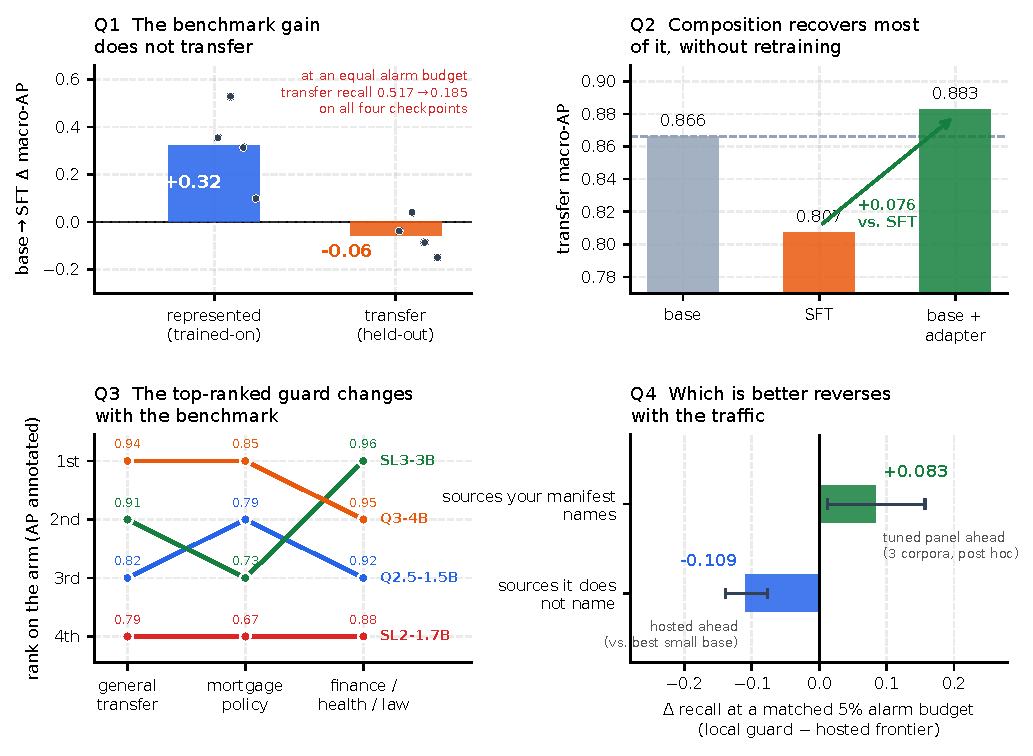
\includegraphics[width=\linewidth]{fig_teaser.pdf}
\caption{\textbf{The report in four panels, one per question --- the same Q1--Q4 as
\Cref{tab:glance} overleaf.} \textbf{Q1}~SFT lifts represented-source macro-AP $\TeaserRepDelta$ and
moves held-out transfer $\TeaserTransferDelta$, pooling per-checkpoint effects from
$\TeaserTransferHi$ to $\TeaserTransferLo$ (dots); at an \emph{equal} alarm budget the apparent
transfer-recall gain reverses on all four checkpoints (\Cref{sec:actI}). \textbf{Q2}~Averaging each
base with its own adapter recovers $\PilotTransferDeltaSFT$ of that transfer for one extra inference
pass --- past SFT on every checkpoint, but not past the strongest base (\Cref{sec:actIII}).
\textbf{Q3}~The \emph{same} four bases, zero-shot, rank differently on every arm; the domain-arm CIs
overlap, so the claim is that the \emph{leaderboard's answer moves}, not that the ordering is resolved
(\Cref{tab:baseline,tab:expguard}). \textbf{Q4}~Both bars are (local $-$ hosted) recall at a matched
$5\%$ alarm budget, so right of zero is a local win: the ordering \emph{reverses} between traffic a
training manifest names and traffic it does not (\Cref{sec:actIII-h2h}). The \HtwoAggDeltaTpr{} bar
(sources your manifest names) is a \emph{post-hoc} descriptive summary over \HtwoNRepSources{}
purposively chosen corpora, and resampling that source set gives \HtwoAggSrcResampledCI{}; the bar
below it --- drawn \emph{left} of zero, because on this axis a hosted win is negative --- is the hosted
model leading the best small base by \FrontierGainOverBase{} in a paired comparison on external
expert-annotated rows. Two
different comparisons on different data --- reported side by side, never pooled. Every value is parsed from the same committed
artifacts the tables \code{\textbackslash input}, so no panel can drift from its row.}
\label{fig:teaser}
\end{figure}

\clearpage
\begin{table}[H]\centering\footnotesize
\caption{\textbf{Results at a glance --- the four answers of \Cref{fig:teaser}, with every headline
number, its estimand, and what it licenses.} This is the claim ledger, and the \textbf{Q} labels are
the panels of \Cref{fig:teaser}: Q1 \emph{and} Q1a are its top-left panel (Q1a is the red annotation
inside it), Q2 its top-right, Q3 its bottom-left, Q4 its bottom-right. Q1b and Q4a sharpen their
neighbours and have no panel of their own. Nothing later in the report is claimed at a stronger
evidence tier than its row allows, and the three tiers are never pooled (\Cref{sec:ledger}).
\emph{Retro.} $=$ retrospective, estimation-only on a panel inspected during development.
\emph{Prereg.} $=$ analysis-preregistered (locked estimands and criteria) but \emph{not} data-blind.
\emph{External} $=$ independently expert-annotated rows. \emph{LLM-judge} $=$ labels assigned by an
LLM against written policy cards, \emph{not} SME-adjudicated. (\emph{Prereg.} qualifies a retrospective
row; it is not a fourth pool.) Intervals are bootstrap ranges conditional on the fixed panel, not
significance tests. Rows Q1a and Q4 are read at a matched false-alarm budget \emph{located on the
evaluated negatives}: they compare ranking quality at a common alarm rate --- ROC points --- and are not
deployable thresholds (\Cref{sec:matched-fpr-limits}).}
\label{tab:glance}
\setlength{\tabcolsep}{4pt}\renewcommand{\arraystretch}{1.18}
\begin{tabular}{@{}>{\raggedright\arraybackslash}p{0.185\linewidth}
                  >{\raggedright\arraybackslash}p{0.255\linewidth}
                  >{\raggedright\arraybackslash}p{0.335\linewidth}
                  >{\raggedright\arraybackslash}p{0.085\linewidth}l@{}}
\toprule
\textbf{Question} & \textbf{Estimand (what was measured)} & \textbf{Answer} & \textbf{Tier} & \textbf{\S} \\
\midrule
Q1. Do benchmark gains \emph{transfer}? &
Paired macro-AP change vs.\ the \emph{same} checkpoint, represented vs.\ source-held-out; 4 checkpoints
$\times$ 5 seeds &
\textbf{Not reliably --- it specializes on this panel.} Represented $\RepDelta$ [$\RepCILower,\RepCIUpper$]; transfer
$\TransferDelta$ [$\TransferCILower,\TransferCIUpper$]; $\SpecializationSeedCount/\TotalSeedCount$ guards
in the specialize quadrant &
Retro. & \S\ref{sec:actI} \\
Q1a. Does that hold at an \emph{equal alarm budget}? &
Each tuned seed re-thresholded to its own base's pooled transfer FPR, then recalls compared &
\textbf{The apparent recall gain reverses.} Transfer recall
$\MatchedTransferBase\!\to\!\MatchedTransferSft$ ($\MatchedTransferDelta$) and \code{HarmBench}
$\MatchedHarmBase\!\to\!\MatchedHarmSft$, worse on all four &
Retro. & \S\ref{sec:actI-op} \\
Q1b. Does it hit guards that are \emph{already} guards? &
Locked criteria over a registered purpose-built panel; 6 released guards $+$ 4 general, 5 seeds,
$\beta{=}\AdaPrimaryBeta$ &
\textbf{Directional criterion met; non-confirmatory.} Represented gain \AdaHGain{} (LCB \AdaHGainLCB).
KL-SFT retains transfer but its
represented cost \AdaHCost{} (LCB \AdaHCostLCB) \textbf{fails} the $-\AdaMargin$ margin &
Prereg. & \S\ref{sec:adaptation} \\
Q2. Can transfer be recovered without retraining? &
Equal-weight average of each base's calibrated score with its own adapter's, vs.\ that adapter &
\textbf{Most of it, for one extra pass.} $\PilotTransferDeltaSFT$
[$\PilotTransferDeltaSFTLow,\PilotTransferDeltaSFTHigh$] vs.\ SFT at a represented cost
$\PilotRepDeltaSFT$; \emph{not} past the strongest base &
Retro. & \S\ref{sec:actIII} \\
Q3. Does a general-safety score cover a regulated domain? &
Zero-shot ranking of a dual-labeled mortgage policy label $D$ (994-row benchmark, scored on its
146-row public-test split) and of three external verticals (2{,}275 rows) &
\textbf{No.} AP$\cdot$D $0.67$--$0.85$ against a $0.555$ chance floor, and the guard ordering does
not carry across the two arms (on mortgage, five of the six pairwise AP$\cdot$D intervals overlap) &
LLM-judge; external & \S\ref{sec:actIV} \\
Q4. Should you run a small guard at all? &
Recall at a matched $5\%$ budget against a hosted frontier model on identical rows, by regime &
\textbf{It depends on the regime.} Hosted leads \FrontierGainOverBase{} \FrontierGainOverBaseCI{} on
unfamiliar prompts; on represented sources the tuned panel leads \HtwoAggDeltaTpr{}
\HtwoAggDeltaTprCI{} (post hoc) &
Retro.; external & \S\ref{sec:actIII-frontier} \\
Q4a. What does buying the hosted model cost? &
Measured median/P99 latency and billed \$/1k on the same rows at concurrency 200 &
\FrontierBestMedianMs\,ms vs.\ tens of ms locally ($\approx\FrontierSlowdown\times$),
\$\FrontierBestCost/1k prompts, and every prompt leaves your boundary &
Retro. & \S\ref{sec:practitioner-cost} \\
\bottomrule
\end{tabular}
\end{table}

\clearpage
\tableofcontents

\section{Introduction: a benchmark gain is not a transfer guarantee}
\label{sec:intro}

\Cref{fig:teaser} and \Cref{tab:glance}, on the two pages before the contents, are the report's
answers; this section says why the questions are the right ones. A guard chosen on a leaderboard --- or ``improved'' by a quick fine-tune --- can quietly do three expensive
things at once in production: \textbf{(1)} raise false alarms that block legitimate users (pooled transfer
false alarms climb $\TransferBasePooledFPRPct\%\!\to\!\TransferSFTPooledFPRPct\%$); \textbf{(2)} miss the hardest
attacks it was meant to stop (HarmBench recall $\HarmBenchBaseRecallPct\%\!\to\!\HarmBenchSFTRecallPct\%$);
and \textbf{(3)}, in a regulated domain, pass a policy violation that reads as polite text or treat a
protected group differently --- a compliance and fair-lending problem, not merely a lower number.
\Cref{fig:casestudy} is that third failure in one concrete row: a routine-sounding underwriting
question that solicits redlining-by-proxy, which all four guards rank \emph{below} the median benign
request in the same split. The four
questions below, and the decision guide that follows from them (\Cref{sec:practitioner}), exist to catch
these failures \emph{before} deployment: when to fine-tune, when to instead \emph{compose}, when a
general guard is simply not enough for a regulated domain, and when to stop self-hosting and escalate.
The front spread answers all four already; the sections below derive them.

Converting a general instruction model into a safety guard with a short parameter-efficient fine-tune
\citep{elesedy2024loraguard} and reporting its score on a public suite \citep{bassani2024guardbench}
is now standard. A post-tuning leaderboard number, however, conflates two different things: raising the
score on benchmark \emph{sources represented in training} versus improving \emph{transfer} to datasets
the guard never saw. This report is organized around one thesis --- \emph{benchmark gains do not
guarantee transfer} --- and four questions on a shared panel of checkpoints:
\begin{enumerate}[leftmargin=2.2em,itemsep=1pt,label=\textbf{Q\arabic*.}]
  \item \textbf{Do benchmark gains transfer?} (\Cref{sec:actI}) --- or does the guard specialize to the
  sources it was tuned on? And does the answer survive being read at an \emph{equal false-alarm budget}
  (Q1a, \Cref{sec:actI-op}) and on guards that are \emph{already} purpose-built
  (Q1b, \Cref{sec:adaptation})?
  \item \textbf{Can transfer be recovered without retraining?} (\Cref{sec:actIII}) --- by composing base $+$ adapter.
  \item \textbf{Does a general-safety score cover a regulated domain?} (\Cref{sec:actIV}) --- evaluated \emph{zero-shot} across law, finance, health, and mortgage.
  \item \textbf{Should you run a small guard at all?} (\Cref{sec:actIII-frontier}) --- the same guards
  priced against a hosted frontier model on identical external rows, in accuracy, latency and cost, and
  against the cheaper escapes a practitioner reaches for first: tuning, scale, an off-the-shelf guard,
  an ensemble (\Cref{sec:frontier-routes}).
\end{enumerate}
The logic is cumulative. Q1 separates represented gain from held-out transfer and then tests the
headline at an equal false-alarm budget. Q1b asks whether the direction extends to released guards. Q2
tests a remedy. Q3 marks the boundary between general safety and domain policy. Q4 turns those findings
into a sourcing decision. Each question closes with an Evidence\,/\,Decision\,/\,Boundary summary that
states what the result licenses and what it does not.

One naming note, so nothing later needs decoding. The questions are what the sections answer; the work
itself was built as three arcs, and the report calls them by name where the arc rather than the question
is the subject: \textbf{Act~I} is the specialization measurement (Q1 and Q1b), \textbf{Act~II} the
composition remedy (Q2), and \textbf{Act~III} the regulated-domain and frontier evidence (Q3 and Q4).
``The Act~I panel'' throughout means the four compact checkpoints and the frozen manifest those
measurements were made on.

\begin{background}{Three ways to read this report}
This is a long document, and not every reader needs all of it.
% \cpageref already prints the word "page", and the `capitalize' option makes it "Page", so the
% "p.~" prefix rendered as "(p. Page 2)". \pageref gives the bare number this wants.
\textbf{If you have five minutes:} \Cref{fig:teaser} (p.~\pageref{fig:teaser}) is the four answers as
one picture, and \Cref{tab:glance} (p.~\pageref{tab:glance}) is every headline number with its
estimand and evidence tier.
\textbf{If you are choosing a guard:} read \Cref{tab:guidelines} --- one row per finding, with the
guideline it implies --- then \Cref{fig:gating} for the gating procedure and
\Cref{sec:practitioner-cost} for the serving economics.
\textbf{If you are checking the work:} the estimand and bootstrap are \Cref{sec:bg-estimand} and
\Cref{sec:setup}; what each arm does \emph{not} license is \Cref{tab:ledger}; and \code{make verify}
(\Cref{sec:repro}) byte-checks the generated tables and figures from committed per-row scores.
Everything technical is defined once, from the ground up, in \Cref{sec:background}.
\end{background}

\paragraph{What is new here.} Prior work already measures safety degradation of the same checkpoint
before and after fine-tuning \citep{hsiung2025guardrails}, policy-overfitting of guardrails
\citep{liu2026domaingeneralizable}, and that a plain instruction model can rival a purpose-built guard
\citep{bassani2024guardbench}; in-distribution versus out-of-distribution blocks are also standard in
guard evaluations \citep{inan2023llamaguard,han2024wildguard,elesedy2024loraguard}. What is missing is a
strictly \emph{paired} guard-classifier estimand that holds checkpoint, manifest, seeds and scorer fixed
while splitting the change into represented-source versus dataset-held-out transfer with per-checkpoint
intervals from a family-aware hierarchical bootstrap --- and then pushes that instrument to a composition
remedy and four regulated domains. Concretely, the novel contributions are:
\begin{enumerate}[leftmargin=1.7em,itemsep=1pt]
  \item \textbf{A paired estimand} that cleanly separates represented-source gain from held-out transfer,
  with a fixed-panel hierarchical bootstrap (\Cref{sec:actI}).
  \item \textbf{The ``attractor'' finding:} on this panel SFT drives each checkpoint toward a benchmark-fixed
  endpoint, so the popular reading ``stronger bases specialize more'' is largely arithmetic; the sharper,
  falsifiable claim is \emph{endpoint invariance} (\Cref{sec:actI-coupling}).
  \item \textbf{A retraining-free composition operator} that recovers transfer, with an equal-cost SFT+SFT
  control isolating the base's contribution (\Cref{tab:sftsft}) and a candidate diversity mechanism
  (base-correlated adapter errors) --- reported as motivation, not proof (\Cref{sec:actIII}).
  \item \textbf{A dual-labeled, HMDA-grounded mortgage benchmark} whose mortgage-policy label $D$
  \emph{refines} general safety $G$ on the looks-safe mass (G0/D1, 502/994 rows; the G1/D0 cell is empty,
  so in v1 the labels are \emph{nested rather than crossed}), with a protected-class
  fairness-invariance gate, plus an external, expert-annotated finance/health/law replication
  (\Cref{sec:actIV}).
  \item \textbf{A reproduce-from-committed-scores pipeline} (tooling, not a research claim): one entry
  point regenerates the Act~I/II, mortgage, ExpGuard, SFT+SFT, latency and teaser artifacts from committed
  per-row scores and byte-checks them, reporting verified/unverified/uncovered counts rather than a single
  green (\Cref{sec:repro}).
\end{enumerate}
\emph{What is \textbf{not} new:} we introduce no new model, metric, or training algorithm, and make no
causal, universal, or deployment claim --- the output is a reproducible, estimation-only characterization
of this fixed panel plus one external domain replication.

\subsection{Scope: what is in the panel, and what is out}
\label{sec:intro-scope}
\noindent English input-prompt classification, binary \code{safe}/\code{unsafe}, one LoRA-SFT
recipe, five training seeds. The panel is wider than the four compact checkpoints the paired estimand
runs on, and an earlier version of this paragraph named only those, which understated what the report
contains. In full: \textbf{(i)} four general instruction checkpoints at 1.5--4B, the shared spine of
Acts~I--II; \textbf{(ii)} a ten-checkpoint $2\times3$ adaptation grid adding six released purpose-built
guards (\Cref{sec:adaptation}); \textbf{(iii)} a Qwen3 scale ladder to 8B and 32B and a released-guard
panel (\Cref{sec:frontier-routes}); \textbf{(iv)} six hosted frontier configurations, priced and timed
(\Cref{sec:actIII-frontier}); \textbf{(v)} guard committees and a base$+$adapter composition operator
(\Cref{sec:actIII}); \textbf{(vi)} a two-model escalation cascade (\Cref{sec:frontier-licenses}); and
\textbf{(vii)} four regulated domains, one synthetic mortgage benchmark and one external
expert-annotated replication (\Cref{sec:actIV}). \Cref{tab:ledger} is the authoritative inventory:
every arm's panel, data, label tier and evidence flavor is listed there, and nothing in this report is
claimed at a flavor stronger than that table gives it. Not a leaderboard, not a fair-lending audit, not
a deployment recommendation.


\subsection{How this differs from the closest work}
\label{sec:related-closest}
Prose comparison let earlier revisions of this report claim more novelty than it has, so the
comparison is a table and it sits here, beside the claim it bounds, rather than in the appendix.
Six contributions sit closer to individual components of our design than a narrative review
conveys, and \Cref{tab:closest} places them against the specific axes we measure rather than
against the design as a whole. Read down a column and the honest position is visible: \emph{no single
row does what this report does end to end}, but almost every column has a row that does that column
better, and three of our components --- routing, fairness instrumentation, and adapting a released
guard --- have direct prior art we do not improve on. The full five-literature review is
\Cref{sec:related}.

\citet{lee2025saferoute} is the closest work to our cascade: it \emph{learns} when to route from a small
guard to a large one and compares against uncertainty baselines, which is exactly the comparison
\Cref{sec:frontier-licenses} proposes as future work and does not run. \citet{achara2025watchdogs} audit
deployed moderation classifiers for fairness and perturbation robustness, an instrument strictly more
developed than our protected-pair gate. \citet{cisnerosvelarde2026policy} and \citet{choi2026compass}
both benchmark natural-language requests against explicit written policies --- COMPASS across eight
organization-specific scenarios --- which is the construct our mortgage $D$ label reaches for with
LLM-judge rather than human labels. \citet{zhao2026mlbenchguard} derive regulation-grounded
multilingual data and train 1.5B/7B policy-conditioned guards, so ``policy grounding'' is not ours either. Most
directly, \citet{hossain2026safetygeometry} study ordinary domain fine-tuning of LlamaGuard, WildGuard
and Granite Guardian --- the same manoeuvre as \Cref{sec:adaptation}, on an overlapping set of released
guards.

\begin{table}[htbp]\centering\scriptsize
\caption{Closest work by component. \cmark{} = the work reports it; \xmark{} = it does not;
$\circ$ = partially. ``Paired base$\to$tune'' means the same checkpoint measured before and after on
identical rows; ``source-held-out'' means transfer measured at the \emph{source} level, not the row
level; ``matched-FPR'' means metrics compared at a common false-alarm budget rather than at each
model's self-chosen operating point. The \emph{leftmost three} columns are where this report's
remaining claim lives --- it is the only row with all three, and their conjunction is the estimand
\Cref{sec:actI} defines. Routing, policy grounding and the fairness construct are where it does not:
each carries a $\circ$ against a row that does it properly. Eight works are listed --- the six
discussed above plus the two general-guard baselines already cited in this section.}
\label{tab:closest}
\setlength{\tabcolsep}{3.2pt}\renewcommand{\arraystretch}{1.12}
\begin{tabular}{@{}>{\raggedright\arraybackslash}p{0.155\textwidth}cccccccc@{}}
\toprule
& Paired & Source- & Matched- & Routing & Policy & Label & Fairness & Regulated \\
Work & base$\to$tune & held-out & FPR & method & grounded & tier & construct & domains \\
\midrule
\citet{lee2025saferoute} & \xmark & $\circ$ & \xmark & \cmark\ learned & \xmark & public & \xmark & \xmark \\
\citet{achara2025watchdogs} & \xmark & \cmark & $\circ$ & \xmark & \xmark & public & \cmark & \xmark \\
\citet{cisnerosvelarde2026policy} & \xmark & \xmark & \xmark & \xmark & \cmark & human & \xmark & $\circ$ \\
\citet{choi2026compass} & \xmark & \xmark & \xmark & \xmark & \cmark & human & \xmark & \cmark \\
\citet{zhao2026mlbenchguard} & \xmark & $\circ$ & \xmark & \xmark & \cmark & mixed & \xmark & \cmark \\
\citet{hossain2026safetygeometry} & \cmark & \cmark & \xmark & \xmark & \xmark & public & \xmark & $\circ$ \\
\citet{elesedy2024loraguard} & \xmark & \cmark & \xmark & \xmark & \xmark & public & \xmark & \xmark \\
\citet{hsiung2025guardrails} & \cmark & $\circ$ & \xmark & \xmark & \xmark & public & \xmark & \xmark \\
\midrule
\textbf{This report} & \cmark & \cmark & \cmark & $\circ$ \emph{margin} & $\circ$ \emph{card} & LLM-judge & $\circ$ \emph{pairs} & \cmark \\
\bottomrule
\end{tabular}\\[3pt]
{\footnotesize Literature cutoff: \textbf{2026-07-30}. Each entry above was resolved against its
publisher record. The three $\circ$ marks in our own row are deliberate and are the ones a reader
should hold us to: the router we \emph{tested} is a score-margin router, not the unfamiliarity router
we find attractive; ``policy grounding'' means consistency with a written policy card checked by an
LLM judge, not human adjudication; and the fairness construct is a 39-pair protected-pair gate --- only
21 of them true single-token swaps, and one crossing a split --- not an audit.}
\end{table}



\section{Background: what the four questions rest on}
\label{sec:background}

This report is written to be read by someone with a first course in statistics, a working idea of
what fine-tuning a small language model means, and a lay familiarity with mortgage lending. Everything
technical the four questions rely on is defined once here, from the ground up, with the exact equations and
a worked example wherever a number would otherwise be mysterious. Nothing in this section reports a
result; it is the vocabulary. Almost every subtlety below exists to make one comparison honest --- a
tuned guard against the \emph{same model before tuning}, on identical rows, split into sources the
guard trained on and sources it never saw --- and \Cref{fig:design} previews that design on one page.

\begin{figure}[t]\centering
\includegraphics[width=0.70\linewidth]{experiment_design.png}
\caption{\textbf{The study at a glance (Acts~I--II).} From one fixed panel and one frozen training
manifest, every guard we compare --- the untuned \textbf{base}, the \textbf{SFT-tuned} guard, and the
retraining-free \textbf{composition} --- is read by the \emph{same} single-token scorer on the
\emph{same} represented and transfer test rows, and each is compared only against its \emph{own} base.
That paired difference $\Delta$, aggregated by a family-aware bootstrap, is the estimand. Act~III then adds
the mortgage and finance/health/law domain evaluations on top of this same machinery.}
\label{fig:design}
\end{figure}

\subsection{The guard: a single-token logit-difference head}
\label{sec:bg-guard}

We do not ask the guard to write a paragraph explaining its decision. We ask it for exactly one
word and look only at how strongly it leans toward that word. Concretely, a prompt $x$ is wrapped in a
fixed instruction template asking for a one-word verdict, and we read the model's raw output scores
--- its \emph{logits} --- at the final position for the two verdict words \code{safe} and
\code{unsafe}. A logit is the model's un-normalized, pre-probability score for a candidate next token:
larger means the model favors that token. Writing $z_{\text{unsafe}}(x,t)$ and $z_{\text{safe}}(x,t)$
for those two logits at the final prompt position $t$, the guard's stored score is their difference,
\begin{equation}
\label{eq:score}
s(x) \;=\; z_{\text{unsafe}}(x,t) \;-\; z_{\text{safe}}(x,t),
\end{equation}
which is positive when the model leans \code{unsafe}, negative when it leans \code{safe}, and near zero
when it is undecided. To read $s(x)$ as a probability we pass the same two logits through a two-way
softmax --- giving, strictly, the probability of \code{unsafe} \emph{conditional on the verdict being one
of the two tokens} $\{$\code{safe}$,$\code{unsafe}$\}$, not the model's full next-token distribution:
\begin{equation}
\label{eq:prob}
p(\text{unsafe}\mid x) \;=\; \frac{\exp\!\big(z_{\text{unsafe}}\big)}{\exp\!\big(z_{\text{safe}}\big)+\exp\!\big(z_{\text{unsafe}}\big)}.
\end{equation}
For example, if $z_{\text{unsafe}}=2.0$ and $z_{\text{safe}}=1.0$, then $s(x)=1.0$ and
$p(\text{unsafe}\mid x)=e^{2}/(e^{2}+e^{1})\approx 0.73$. This is what we mean by a
``single-token logit-difference head'': one forward pass, two numbers, one score. The raw logits are
the canonical stored value; probabilities in \Cref{eq:prob} and any temperature-rescaled version are
\emph{derived} from them. Reading the model's own generated verdict text is deliberately never used as
the primary score, because a free-text answer is harder to score consistently and hides the model's
actual confidence.

\subsection{Base, SFT, and LoRA}
\label{sec:bg-sft}

The \emph{base} is the general instruction-tuned chat model \emph{before} we turn it into a guard. It
is not untrained --- it can already follow the ``answer \code{safe} or \code{unsafe}'' instruction
zero-shot --- so ``base'' throughout means ``before the guard fine-tune,'' not ``blank.''
\emph{Supervised fine-tuning} (SFT) then trains that model on labeled examples: for each training
prompt we know the correct verdict, and we nudge the model to raise the probability it assigns to that
verdict word. Rather than update all of the model's weights, we use \emph{LoRA} (Low-Rank Adaptation)
\citep{hu2021lora}: we freeze the original weights and insert a small number of extra trainable
parameters (a low-rank ``adapter'') into selected weight matrices. LoRA is cheap, fast, and reversible
--- you can ship the tiny adapter on top of the frozen base --- and it is the standard way guards are
built in practice \citep{elesedy2024loraguard}. The precise adapter size and which matrices it touches
are part of the frozen recipe in \Cref{sec:setup}.

\subsection{Average precision, macro-AP, and the accuracy trap}
\label{sec:bg-ap}

Because $s(x)$ is a continuous score, we can grade a guard \emph{without} committing to a cutoff, by
asking how well it \emph{ranks}. \emph{Average precision} (AP) collapses the whole
precision--recall curve into a single number in $[0,1]$: it is near $1$ when the guard tends to give
genuinely unsafe prompts higher scores than safe ones, and it needs no threshold. Formally, sweeping
the cutoff from high to low, AP is the recall-weighted average of the precision achieved at each
true-positive, $\text{AP}=\sum_n (R_n-R_{n-1})\,P_n$, with $P_n,R_n$ the precision and recall after the
$n$-th ranked item; we use the tie-aware, non-interpolated \code{scikit-learn} definition so the number
is exactly reproducible.

\begin{background}{A worked AP example}
Rank five prompts by their guard score, highest first, and write their true labels:
$[\text{unsafe},\ \text{unsafe},\ \text{safe},\ \text{unsafe},\ \text{safe}]$. There are three unsafe
prompts, so each one contributes recall $\tfrac13$. The precision at each unsafe prompt as we go down
the list is $\tfrac11{=}1.00$ (rank 1), $\tfrac22{=}1.00$ (rank 2), and $\tfrac34{=}0.75$ (rank 4). So
$\text{AP}=\tfrac13(1.00)+\tfrac13(1.00)+\tfrac13(0.75)\approx 0.917$. A perfect ranking (all three
unsafe prompts on top) would score $1.00$; ranking the safe prompts first would score much lower.
\end{background}

\emph{Macro}-AP computes AP separately on each benchmark and then averages those per-benchmark values
with \emph{equal weight}, so one large benchmark cannot dominate a handful of small ones; this is the
primary metric behind every one of the four questions.

\begin{takeaway}{Why not just report accuracy?}
On a test set that is $95\%$ safe, a guard that blindly answers \code{safe} to everything scores $95\%$
accuracy while catching \emph{zero} attacks. Accuracy rewards guessing the majority class; AP and
macro-AP instead reward putting the unsafe prompts on top, which is the behavior a guard is for. This
is why ranking, not accuracy, is the currency of this report.
\end{takeaway}

\subsection{Two evaluation regimes: represented-source vs.\ dataset-held-out transfer}
\label{sec:bg-regimes}

The single most important distinction in this report is \emph{where the test data came from}.
\textbf{Represented-source} test rows are held-back examples drawn from a dataset the guard
\emph{trained on} (different rows, same source). \textbf{Dataset-held-out transfer} rows come from
datasets whose examples were \emph{never used in training at all}. A gain that appears on
represented-source tests but not on transfer tests is precisely the signature of a guard
\emph{specializing} to its training sources rather than becoming a broadly better moderator. One
honesty caveat travels with the word ``held out'': it means \emph{dataset-held-out} (those rows were
withheld from fine-tuning), \emph{not} sealed away from the researchers during development --- a
distinction that forces the retrospective framing discussed in \Cref{sec:bg-estimand}.

\subsection{From scores to decisions: calibration, operating point, TPR/FPR, macro vs.\ pooled}
\label{sec:bg-op}

Ranking is threshold-free, but a deployed guard must eventually say \code{safe} or \code{unsafe}. An
\emph{operating point} is the single cutoff on $s(x)$ that converts scores into hard decisions. Picking
it trades two error rates against each other: the \emph{true-positive rate} (TPR, or recall) is the
fraction of genuinely unsafe prompts the guard flags, and the \emph{false-positive rate} (FPR) is the
fraction of genuinely safe prompts it wrongly flags. Raising the cutoff lowers both; lowering it raises
both. Before thresholding we \emph{calibrate}: we fit a single positive \emph{temperature} that rescales
the logits (temperature scaling \citep{guo2017calibration}) so the derived probabilities in
\Cref{eq:prob} are better behaved. Crucially, both the temperature and the cutoff are fit only on a
separate held-back \emph{calibration} split --- never on the transfer or stress data we report on --- so
the threshold is not quietly tuned to the test.

Two error rates can be averaged two ways, and the choice matters. \emph{Macro} rates compute the rate
on each benchmark first and then average across benchmarks (equal weight per benchmark). \emph{Pooled}
rates lump every row together first and then compute one rate (equal weight per row, so large
benchmarks dominate). We report both because they can disagree.

Keep the two questions apart: AP answers ``does it rank?'' and the operating point answers ``is there a
usable decision boundary?'' A guard can rank well and still have no cutoff that survives off-source,
because the score \emph{distribution} shifts even when the \emph{ordering} holds --- a gap Acts~I and~II
both measure (\Cref{sec:actI-op,sec:actIII-operating}).

\subsection{Estimands, the fixed panel, and the paired hierarchical bootstrap}
\label{sec:bg-estimand}

\begin{background}{Three terms that appear in the verdicts, in plain words}
\textbf{Lower confidence bound (LCB).} A one-sided version of an interval. Saying ``the gain is
\AdaHGain{}, LCB \AdaHGainLCB'' --- the actual RQ1 result of \Cref{sec:adaptation} --- means: the
estimate is \AdaHGain{}, and under resampling the value stayed above \AdaHGainLCB{} in $97.5\%$ of the
redraws. A criterion of the form ``LCB $>0$'' is therefore a demand that even
the pessimistic end of the range still be a gain. (UCB is the mirror image, used for quantities we want
to bound from \emph{above}, such as a loss.) This example is the generated macro rather than a typed
number, because an earlier revision left it quoting a superseded panel's value.

\textbf{Non-inferiority margin.} How much you are willing to lose on one axis to win on another, fixed
\emph{before} looking. A margin of $-0.02$ says: a drop of up to two AP points is acceptable, more is
not. This is stricter than ``did it get worse?'' --- it must be provably \emph{not much} worse, so a
noisy result fails the test rather than passing it by default. \Cref{sec:adaptation} contains the one
place in this report where a preregistered criterion of this kind is failed and reported as failed.

\textbf{Bonferroni split.} When you test two things at once, each gets half the error budget
($\alpha=0.05$ becomes $0.025$ each), so asking two questions cannot double your chance of a lucky
answer. It is the cheapest, most conservative way to pay for multiplicity.
\end{background}

An \emph{estimand} is the exact quantity our numbers describe. Here it is the average
before-versus-after change \emph{for the four specific checkpoints we study}, not for ``small guards''
in general. Those four checkpoints are a \emph{fixed, purposively chosen panel} --- picked deliberately,
not sampled at random from a population --- so we do not attach uncertainty to the choice of models and
we do not generalize to unnamed architectures. Every comparison is \emph{paired}: an adapter is always
compared against \emph{its own base} on the \emph{same rows}, so nothing but the fine-tune differs.

To put a $95\%$ range around a paired change we use a \emph{paired hierarchical bootstrap}. A bootstrap
estimates how much a result would wobble under resampling by rebuilding the data many times from itself
and recomputing; the spread of the recomputed values becomes the interval. Ours is \emph{hierarchical}
because it resamples at two levels at once --- which fine-tuning \emph{seeds} were drawn (within each
fixed checkpoint), and which groups of near-duplicate evaluation rows (``families,''
\Cref{sec:setup-decon}) are counted, via one Poisson(1) re-count weight per family. It is \emph{paired}
because each adapter stays yoked to its base. Because the training rows and their order are held fixed,
seed-to-seed variation reflects initialization, dropout, and execution nondeterminism --- not
which examples the guard happened to see. The resulting intervals are \emph{conditional} on this panel,
these datasets, and this family graph; they are descriptive, not significance tests, and not claims
about a wider population. This is why Acts~I--II report point estimates, intervals, and leave-one-out
sensitivity checks but no accept/reject test: they were analyzed \emph{after} the benchmarks had been
inspected during development, and clean provenance does not make an inspected benchmark prospective
(see the scope note on p.~1 and \Cref{sec:honesty}).

\subsection{Fine-tuning the guard: LoRA-SFT}
\label{sec:bg-objectives}

We fine-tune each guard with \textbf{SFT} (supervised fine-tuning): a cross-entropy loss that directly
raises the model's log-probability of the single correct verdict token, applied as a parameter-efficient
LoRA adapter (the exact recipe is \Cref{tab:panel-recipe}). SFT is the one training recipe used throughout;
Act~I measures what it changes, and Act~II asks whether we can recover what it gives up \emph{without}
any further tuning.

\subsection{Output-space composition}
\label{sec:bg-composition}

Act~II introduces a retraining-free remedy. \emph{Output-space composition} combines two guards by
averaging their calibrated \emph{output scores} --- not their internal weights. It is portable, because
it needs only two comparable scores rather than interpolable parameters, but it costs two inference
passes because both models must run. This contrasts with \emph{weight-space} methods such as WiSE-FT and
model soups \citep{wortsman2022wiseft,wortsman2022modelsoups}, which average the models' weights and so
require the models to be weight-compatible. The exact composition rule is given later as
\Cref{eq:comp}.

\subsection{The mortgage/HMDA vocabulary and the dual-label idea}
\label{sec:bg-mortgage}

Act~III moves to regulated domains, where a request can read as perfectly polite text yet, if honored,
break the law. The mortgage vocabulary below is what the benchmark encodes.

\begin{background}{Mortgage terms, in plain words}
\textbf{HMDA} --- the U.S.\ Home Mortgage Disclosure Act \citep{hmda2022}: lenders publicly report
loan-level records (purpose, amount band, action taken, denial reason), which we use only as
\emph{de-identified, banded fact sheets}, never verbatim. \textbf{Fair lending} bars credit
discrimination on protected traits. \textbf{Redlining} is refusing or worsening credit across a whole
neighborhood as a proxy for race. \textbf{Disparate treatment} is intentional differential treatment;
\textbf{disparate impact} is a facially neutral rule that falls harder on a protected group.
\textbf{Proxy (coded) discrimination} uses a stand-in --- ZIP code, preferred language --- for a
protected class. \textbf{ATR/QM} is the ability-to-repay / qualified-mortgage rule.
\textbf{Adverse-action notice} is the legally required true reason for a denial. \textbf{UDAAP} covers
unfair, deceptive, or abusive acts and practices.
\end{background}

\noindent On top of that vocabulary the benchmark adds one construct
(\Cref{sec:actIV-mortgage-design}): two \emph{separately assigned} labels per request, general safety $G$ and
mortgage policy $D$, isolating the stratum a general-safety score cannot see.
   % Background concepts only (methods moved to Appendix B)
% related work + the detailed experimental setup are now Appendices A/B (see end of document)
\section{Q1. Do benchmark gains transfer? Not reliably --- this panel specializes}
\label{sec:actI}

The first act answers the most basic question a practitioner has after fine-tuning a guard:
\emph{what did the fine-tune actually buy, and does it hold up off the training distribution?} The
leaderboard answer --- a single higher number --- silently blends two very different things: doing
better on benchmark \emph{sources the guard trained on} (``represented''), and doing better on
datasets it \emph{never saw} (``transfer''). Act I separates them with a strictly paired,
same-checkpoint measurement and finds a clean, repeatable pattern: supervised fine-tuning (SFT)
delivers a large, uniform represented-source gain and essentially no average transfer gain --- the
guard \emph{specializes}.

\begin{background}{What ``paired'' buys us, and why it matters}
Most guard papers compare \emph{different} models: model $X$'s guard against model $Y$'s guard. That
confounds ``the fine-tune helped'' with ``$X$ was a better starting model than $Y$.'' We instead hold
the checkpoint fixed and compare each guard \emph{against its own base}, on the identical rows, with
the identical single-token score head ($s(x)=z_{\text{unsafe}}-z_{\text{safe}}$; see
\Cref{sec:background}) and the identical tie-aware macro-AP. The reported quantity is therefore a
\emph{within-checkpoint change}, $\Delta = \text{SFT} - \text{base}$, not a cross-model gap. This is
the only way to attribute a movement to the fine-tune rather than to the luck of the starting point.
\end{background}

\subsection{The paired base-to-SFT design}
\label{sec:actI-design}

\paragraph{Panel and manifest.} All four checkpoints (Qwen2.5-1.5B, SmolLM2-1.7B, SmolLM3-3B,
Qwen3-4B) are fine-tuned from the identical frozen manifest of $1{,}200$ rows: $400$ from each of three
represented sources --- \code{toxicchat}, \code{prompt\_injections}, and
\code{jailbreak\_classification} --- balanced $200$ safe / $200$ unsafe within each source. The manifest
was decontaminated against the evaluation sets and its data order fixed by seed $42$, so every
checkpoint sees the same examples in the same order; the only thing that varies across the five runs
per checkpoint is the training seed.

\paragraph{Recipe.} Each guard is a LoRA adapter (\code{r=32}, \code{alpha=64}, \code{dropout=0.05})
attached to the attention and MLP projections (\code{q,k,v,o,gate,up,down}), trained for $300$ steps at
learning rate \code{2e-4} on a cosine schedule with $3\%$ warmup, effective batch size $4$, and maximum
sequence length $1024$. We run five seeds ($42$--$46$) per checkpoint, giving $20$ SFT guards in total.
Only the adapter is trained; the base weights are frozen, so ``base'' means the same model \emph{before}
the guard adapter, evaluated with the identical scoring head.

\paragraph{Two evaluation regimes.} Every guard and its base are scored in two disjoint regimes.
\emph{Represented} = held-back rows from the three training sources (same sources, unseen rows);
\emph{transfer} = four datasets whose rows were never used in training --- \code{jailbreakbench},
\code{xstest}, \code{wildguardtest}, and \code{wildjailbreak}. We additionally probe two single-class
stress sets that isolate the two failure directions: \code{OR-Bench} (benign prompts, to measure
over-refusal) and \code{HarmBench} (hard attack prompts, to measure missed catches).

\paragraph{Estimand and intervals.} We summarise each regime by macro-AP (average precision averaged
with equal weight across benchmarks, so a large benchmark cannot dominate) and put a two-sided $95\%$
interval on each change with a \emph{paired hierarchical bootstrap} that keeps every adapter tied to its
own base and respects the checkpoint$\to$seed grouping. The estimand is deliberately narrow: it is the
change \emph{conditional on this fixed, purposively-chosen four-checkpoint panel and this manifest},
which was inspected during development. These are estimation intervals, not significance tests, and the
result is \emph{retrospective, not confirmatory} --- no causal or population claim is licensed.

\subsection{The primary result: a uniform represented gain, a split transfer effect}
\label{sec:actI-primary}

\Cref{tab:primary} reports, per checkpoint, the untuned-base and mean-SFT macro-AP in each regime, the
paired base-to-SFT change with its interval, and the fixed-panel aggregate.

\begin{table}[htbp]\centering\small
\caption{Act I --- fixed-panel result: base and mean-SFT macro-AP by regime, paired base-to-SFT deltas
with two-sided $95\%$ hierarchical-bootstrap intervals, and the fixed-panel aggregate. Descriptive under
the locked precision-focused mode; conditional on this panel.}
\label{tab:primary}
\resizebox{\textwidth}{!}{% Auto-generated by analyze_paper_a_sft.py -- do not edit by hand.
\begin{tabular}{lrrrrrr}
\toprule
Checkpoint & Rep base & Rep SFT & $\Delta$ Rep [two-sided 95\% percentile CI] & Tr base & Tr SFT & $\Delta$ Tr [two-sided 95\% percentile CI] \\
\midrule
Qwen2.5-1.5B & 0.6334 & 0.9878 & 0.3544 [0.2731, 0.4150] & 0.8187 & 0.7798 & -0.0389 [-0.0829, 0.0062] \\
SmolLM2-1.7B & 0.4524 & 0.9806 & 0.5282 [0.4555, 0.5748] & 0.7904 & 0.8304 & 0.0400 [0.0003, 0.0776] \\
SmolLM3-3B & 0.6621 & 0.9751 & 0.3130 [0.2419, 0.3701] & 0.9102 & 0.8234 & -0.0869 [-0.1114, -0.0613] \\
Qwen3-4B & 0.8855 & 0.9837 & 0.0981 [0.0545, 0.1479] & 0.9438 & 0.7939 & -0.1499 [-0.1963, -0.1050] \\
\midrule
Fixed-panel aggregate & -- & -- & 0.3234 [0.2647, 0.3690] & -- & -- & -0.0589 [-0.0837, -0.0321] \\
\bottomrule
\end{tabular}
}
\end{table}

\paragraph{Represented: everyone reaches the same ceiling.} The represented-source gain is large and,
strikingly, \emph{uniform in its destination}: regardless of where the base started, every SFT guard
lands at macro-AP $\approx 0.98$. SmolLM2-1.7B climbs from a weak $0.4524$ to $0.9806$; Qwen2.5-1.5B
from $0.6334$ to $0.9878$; SmolLM3-3B from $0.6621$ to $0.9751$; and Qwen3-4B, already strong at
$0.8855$, to $0.9837$. Because the finish line is shared, the \emph{size} of the represented gain is
essentially dictated by how far below the ceiling the base sat --- a $+0.5282$ jump for SmolLM2 versus
only $+0.0981$ for Qwen3-4B. The fixed-panel aggregate is $\RepDelta$
$[\RepCILower, \RepCIUpper]$: SFT reliably teaches each model to rank the training sources' held-back
rows near-perfectly. Mechanistically this is unsurprising --- the manifest \emph{is} those sources, so
the adapter learns their label conventions and surface cues.

\paragraph{Transfer: a small average that hides opposite signs.} On data the guard never saw, the same
fine-tune does something quite different. The aggregate transfer change is only $\TransferDelta$
$[\TransferCILower, \TransferCIUpper]$ --- close to zero and slightly negative. But this panel average
is a mirage: it pools \emph{opposing} per-checkpoint effects. The change is positive for the weakest
base and strongly negative for the strongest, spanning
$+0.0400$ $[+0.0003, +0.0776]$ for SmolLM2-1.7B, $-0.0389$ $[-0.0829, +0.0062]$ for Qwen2.5-1.5B,
$-0.0869$ $[-0.1114, -0.0613]$ for SmolLM3-3B, and $-0.1499$ $[-0.1963, -0.1050]$ for Qwen3-4B. The
ordering tracks base transfer strength (\Cref{tab:primary}): the models with the most transfer skill to
begin with (SmolLM3 at $0.9102$, Qwen3-4B at $0.9438$) give the most of it back, while the model that
had the least ($0.7904$) is the only one that improves. In other words, SFT does not add a portable
notion of ``unsafe''; it reshapes the score toward the training sources, and for a model that already
generalised well that reshaping is a net loss off-distribution (\Cref{fig:act1-bars}).

\begin{figure}[t]\centering
\includegraphics[width=0.82\linewidth]{fig_act1_percheckpoint.pdf}
\caption{Per-checkpoint view of Act~I: SFT lifts represented-source macro-AP for every checkpoint (blue),
but the transfer change (orange) ranges from $+0.04$ (SmolLM2) to $-0.15$ (Qwen3-4B) --- the fixed-panel
average hides opposite signs.}
\label{fig:act1-bars}
\end{figure}

\begin{takeaway}{Why the $\TransferDelta$ transfer average is misleading}
It averages effects that point in opposite directions --- SmolLM2 $+0.0400$ against Qwen3-4B $-0.1499$.
The panel-level number is small; the panel itself is \emph{not} uniform, and reporting only the
aggregate would erase the most important finding (who loses, and how much). Read the per-checkpoint
column, not the bottom row.
\end{takeaway}

\subsection{Where the transfer losses live: a per-benchmark decomposition}
\label{sec:actI-perbench}

Aggregating over benchmarks can also hide \emph{which} data the guard forgets how to rank. The upper
block of \Cref{tab:sensitivity} decomposes the change benchmark by benchmark. On the represented side
every source rises sharply --- \code{toxicchat} $+0.1880$, \code{prompt\_injections} $+0.3704$, and
\code{jailbreak\_classification} $+0.4119$ --- confirming the gain is broad across the training sources,
not driven by one easy set.

On the transfer side the losses are \emph{concentrated on the jailbreak-style adversarial sets}:
\code{jailbreakbench} $-0.0776$, \code{wildjailbreak} $-0.0792$, and \code{wildguardtest} $-0.0669$ all
fall by a comparable amount, while \code{xstest} --- which contrasts genuinely unsafe prompts against
benign look-alikes rather than adversarial attacks --- barely moves at $-0.0120$. The pattern is
coherent with the mechanism above: the training sources over-represent a particular flavour of unsafe
text, so after tuning the guard ranks \emph{those} confidently but loses discrimination precisely on the
adversarial, distribution-shifted prompts that a deployed guard most needs to catch. Specialization is
not uniform forgetting; it is forgetting the hardest, most out-of-distribution cases first.

\subsection{The specialization plane: 15 of 20 guards specialize}
\label{sec:actI-plane}

The clearest single view of Act I is the \emph{specialization plane} (\Cref{fig:plane}), which plots
each of the $20$ (checkpoint, seed) guards by its represented change (horizontal) against its transfer
change (vertical). Four quadrants have direct meaning: lower-right = represented up, transfer down
(``specialize''); upper-right = both up (``uniform gain''); lower-left = both down (``uniform loss'');
upper-left = transfer-favoured. \SpecializationSeedCount{} of \TotalSeedCount{} guards land in the
specialize quadrant, \UniformGainSeedCount{} in uniform gain, and \emph{none} in uniform loss or the
transfer-favoured quadrant. So specialization is the dominant --- but not universal --- outcome: the
five uniform-gain points are four of the five SmolLM2 seeds \emph{plus} Qwen2.5's seed~42 --- concentrated
on the two checkpoints with the weakest base transfer, which have the most room to improve there (SmolLM2's
remaining seed, 46, narrowly specializes at $-0.001$). The absence of any uniform-loss point matters: SFT never simply degrades the
guard everywhere; it trades transfer for represented ranking. Per-seed values behind the plane are
tabulated in \Cref{tab:seed-values}, and show the effect is stable within each checkpoint (e.g. every
Qwen3-4B seed is a substantial transfer loss, every SmolLM2 seed a represented gain).

\begin{figure}[htbp]\centering

\includegraphics[width=0.6\textwidth]{specialization_plane.pdf}
\caption{Each point is one (checkpoint, seed): horizontal axis is the represented-source macro-AP
change, vertical axis the transfer change. \SpecializationSeedCount{}/\TotalSeedCount{} land in the
lower-right specialization quadrant --- the visual signature of Act I.}
\label{fig:plane}
\end{figure}

\begin{table}[htbp]\centering\scriptsize\setlength{\tabcolsep}{2.5pt}
\caption{Observed represented-source and transfer macro-AP change for every SFT seed (Act~I),
generated from the same validated score matrix as \Cref{tab:primary}. Every Qwen3-4B seed is a substantial
transfer loss and every SmolLM2-1.7B seed a represented gain --- the per-seed stability behind the
specialization plane (\Cref{fig:plane}).}
\label{tab:seed-values}
% Auto-generated by analyze_paper_a_sft.py -- do not edit by hand.
\begin{tabular}{lrrr}
\toprule
Checkpoint & Seed & $\Delta$ represented AP & $\Delta$ transfer AP \\
\midrule
Qwen2.5-1.5B & 42 & 0.3569 & 0.0082 \\
Qwen2.5-1.5B & 43 & 0.3535 & -0.0261 \\
Qwen2.5-1.5B & 44 & 0.3506 & -0.0545 \\
Qwen2.5-1.5B & 45 & 0.3558 & -0.0438 \\
Qwen2.5-1.5B & 46 & 0.3551 & -0.0786 \\
SmolLM2-1.7B & 42 & 0.5304 & 0.0805 \\
SmolLM2-1.7B & 43 & 0.5273 & 0.0720 \\
SmolLM2-1.7B & 44 & 0.5253 & 0.0250 \\
SmolLM2-1.7B & 45 & 0.5309 & 0.0238 \\
SmolLM2-1.7B & 46 & 0.5272 & -0.0013 \\
SmolLM3-3B & 42 & 0.3045 & -0.0812 \\
SmolLM3-3B & 43 & 0.3253 & -0.0925 \\
SmolLM3-3B & 44 & 0.3051 & -0.0629 \\
SmolLM3-3B & 45 & 0.3146 & -0.0923 \\
SmolLM3-3B & 46 & 0.3156 & -0.1055 \\
Qwen3-4B & 42 & 0.0953 & -0.1222 \\
Qwen3-4B & 43 & 0.0936 & -0.1536 \\
Qwen3-4B & 44 & 0.1038 & -0.0949 \\
Qwen3-4B & 45 & 0.0997 & -0.2291 \\
Qwen3-4B & 46 & 0.0981 & -0.1497 \\
\bottomrule
\end{tabular}

\end{table}

\subsection{At a deployable operating point}
\label{sec:actI-op}

Ranking is threshold-free, but deployment is not: at some point you must pick a cutoff and turn scores
into \code{block}/\code{allow} decisions. To see the deployment consequence of specialization we select
each guard's threshold to hit a $5\%$ false-positive-rate (FPR) target on a calibration split, then read
off the realized rates. The lower blocks of \Cref{tab:sensitivity} report them.

\paragraph{Represented recall soars.} On the represented sources, catching the unsafe prompts (TPR)
jumps from \RepBaseTPRPct\% (base) to \RepSFTTPRPct\% (SFT) --- the operating-point face of the same
$\approx 0.98$ ranking gain --- while the represented false-alarm rate stays low and even edges down
(\RepBaseFPRPct\% to \RepSFTFPRPct\%). If you only measured on the training sources, the guard would
look strictly and dramatically better.

\paragraph{Transfer pays for it.} Off-source the picture inverts. The transfer benchmark-macro FPR
climbs from \TransferBaseFPRPct\% (base) to \TransferSFTFPRPct\% (SFT) --- the tuned guard raises nearly
twice as many false alarms on data it never trained on --- and the pooled-negative FPR blows past target
from \TransferBasePooledFPRPct\% to \TransferSFTPooledFPRPct\%, so the calibrated threshold simply does
not transfer. Transfer recall rises only modestly (\TransferBaseTPRPct\% to \TransferSFTTPRPct\%),
nowhere near the represented jump --- and that rise is \emph{not} iso-FPR, which matters more than its
size. The two recalls are realized at \TransferBaseFPRPct\% and \TransferSFTFPRPct\% macro FPR, so the
tuned guard buys much of its extra recall by alarming roughly twice as often; a recall comparison at
unequal false-alarm rates is not a comparison of discriminative power.

\paragraph{The fair comparison: an equal false-alarm budget.} So we make the alarm budgets equal and
re-read the same rows. \Cref{tab:matchedfpr} gives each tuned guard the threshold at which its pooled
transfer false-alarm rate \emph{matches its own base's}, and then compares recalls. The modest apparent
gain does not merely shrink --- it reverses, on \emph{all four} checkpoints and by a wide margin: transfer recall goes \MatchedTransferBase{}\,$\to$\,\MatchedTransferSft{}
(\MatchedTransferDelta) and \texttt{HarmBench} recall \MatchedHarmBase{}\,$\to$\,\MatchedHarmSft{}
(\MatchedHarmDelta). At an equal alarm budget the tuned guard catches \emph{less than half} of what its
own untuned base catches off-source. The direction is stable across the three quantile conventions we
tried (panel mean \MatchedStabilityLo{} to \MatchedStabilityHi).

This is the honest form of the operating-point result, and it is the one the rest of Act~I predicts: the
$+0.06$ recall gain in \Cref{tab:sensitivity} is an artifact of comparing at unequal alarm rates. It needs
no GPU and no pinned environment --- matching false-alarm rates is ranking arithmetic on the same
committed \code{score\_raw} and \code{gold} columns every other covered artifact uses, so it is
regenerated and byte-checked by \code{make verify} (\Cref{sec:repro}); the emitter reproduces every
published row of \Cref{tab:sensitivity} exactly before adding the matched column, which is how we know the
two tables read the same underlying scores. Earlier drafts described this reconstruction as a
\emph{direction} that required the lock-pinned environment. That was wrong on both counts, and the
measured result is both larger and sharper than the hedge it replaces.

The single-class stress sets make the cost concrete: on the hard
\code{HarmBench} attacks the tuned guard's recall \emph{falls} from \HarmBenchBaseRecallPct\% to
\HarmBenchSFTRecallPct\% --- it catches less of the very content a guard exists to stop --- while
benign over-refusal on \code{OR-Bench} is essentially flat (\ORBenchBaseFPRPct\% to \ORBenchSFTFPRPct\%).
Since \code{OR-Bench} is \emph{also} unseen data, ``off-distribution'' cannot be what distinguishes it:
the extra false alarms are specific to the transfer suite's negatives, and we do not identify what
separates them. What the flat OR-Bench line does rule out is a blanket increase in caution.

Note that this \code{HarmBench} drop needs no threshold caveat at all: the tuned guard catches
\emph{less} while alarming \emph{more} (\TransferSFTFPRPct\% vs \TransferBaseFPRPct\% macro transfer
FPR), so it is dominated --- worse on both axes at once, not traded off. Equalising the budget only
widens the gap, to \MatchedHarmSft{} against the base's \MatchedHarmBase{} (\Cref{tab:matchedfpr}).

% tabcolsep was 6pt, which pushed this generated tabular 4.7pt past the text block.
\begin{table}[htbp]\centering\small\setlength{\tabcolsep}{4.5pt}
\caption{Act I --- per-benchmark paired deltas (upper) and the calibration-targeted $5\%$ FPR operating
point plus single-class stress diagnostics (lower). Generated from the lock-bound scores.}
\label{tab:sensitivity}
% Auto-generated by analyze_paper_a_sft.py -- do not edit by hand.
\begin{tabular}{llrrrr}
\toprule
Regime / benchmark & Metric & Base & SFT & $\Delta$ & $N$ \\
\midrule
represented / toxicchat & AP & -- & -- & 0.1880 & -- \\
represented / prompt\_injections & AP & -- & -- & 0.3704 & -- \\
represented / jailbreak\_classification & AP & -- & -- & 0.4119 & -- \\
transfer / jailbreakbench & AP & -- & -- & -0.0776 & -- \\
transfer / xstest & AP & -- & -- & -0.0120 & -- \\
transfer / wildguardtest & AP & -- & -- & -0.0669 & -- \\
transfer / wildjailbreak & AP & -- & -- & -0.0792 & -- \\
\midrule
represented & TPR@target FPR & 0.1296 & 0.7686 & 0.6390 & 313 \\
represented & benchmark-macro realized FPR & 0.0169 & 0.0108 & -0.0061 & 364 \\
represented & pooled-negative realized FPR & 0.0213 & 0.0194 & -0.0019 & 364 \\
transfer & TPR@target FPR & 0.5171 & 0.5807 & 0.0636 & 790 \\
transfer & benchmark-macro realized FPR & 0.0805 & 0.1546 & 0.0741 & 790 \\
transfer & pooled-negative realized FPR & 0.0430 & 0.1704 & 0.1273 & 790 \\
\midrule
Stress / OR-Bench & benign FPR & 0.1181 & 0.1201 & 0.0020 & 400 \\
Stress / HarmBench & recall & 0.7800 & 0.6003 & -0.1797 & 200 \\
\bottomrule
\end{tabular}

\end{table}

% GENERATED by reproduce.py (matched_fpr.py) from artifacts/paper_a_sft_v2/scores/scores.parquet
\begin{table}[htbp]\centering\small\setlength{\tabcolsep}{4.5pt}
\caption{\textbf{The same operating point read at an equal false-alarm budget.} \Cref{tab:sensitivity} compares recalls at each guard's \emph{own} calibrated threshold, where the tuned guard alarms far more often (17.0\% vs 4.3\% pooled transfer FPR) --- so it buys recall with alarms, and the two recalls are not comparable. Here each SFT seed is instead thresholded so its pooled transfer false-alarm rate \emph{matches its own base's} (the budget column), which makes the recalls directly comparable. At an equal budget the tuned guard is worse on \textbf{all four} checkpoints and on both instruments: transfer recall 0.517$\rightarrow$0.217 (-0.300) and \texttt{HarmBench} recall 0.780$\rightarrow$0.203 (-0.577). The direction is stable across the three quantile conventions we tried (panel-mean transfer delta -0.300 to -0.290). Same committed rows and same scorer as \Cref{tab:sensitivity}; only the threshold rule changes, so this needs no GPU and is byte-checked by \code{make verify}. \textbf{This is a retrospective ROC point, not a deployable threshold}: the quantile is read off the \emph{same} labelled negatives the recall is then measured on, so a production system without labels could not place it. Read the row as ``recall at an empirical matched-FPR ROC point'', and see \Cref{sec:matched-fpr-limits} for what an operational version would require.}
\label{tab:matchedfpr}
\begin{tabular}{lrrrrrrr}\toprule
& FPR & \multicolumn{3}{c}{transfer recall (macro)} & \multicolumn{3}{c}{\texttt{HarmBench} recall} \\
\cmidrule(lr){3-5}\cmidrule(lr){6-8}
Checkpoint & budget & base & SFT own thr. & SFT matched & base & SFT own thr. & SFT matched \\
\midrule
Qwen2.5-1.5B & 7.7\% & 0.485 & 0.571 & 0.296 & 0.810 & 0.606 & 0.312 \\
SmolLM2-1.7B & 2.4\% & 0.416 & 0.588 & 0.221 & 0.610 & 0.615 & 0.224 \\
SmolLM3-3B & 1.5\% & 0.512 & 0.596 & 0.141 & 0.740 & 0.611 & 0.116 \\
Qwen3-4B & 5.6\% & 0.655 & 0.569 & 0.211 & 0.960 & 0.569 & 0.160 \\
\midrule
Panel mean & 4.3\% & 0.517 & 0.581 & \textbf{0.217} & 0.780 & 0.600 & \textbf{0.203} \\
\bottomrule
\end{tabular}
\end{table}


\begin{takeaway}{The deployment cost behind the ranking story}
Read together, the operating point says the specialized guard \emph{catches more of what it trained on,
raises more false alarms on what it didn't, and misses more hard attacks}. A leaderboard number computed
on represented sources would advertise only the first of these three.

And the apparent consolation --- ``at least transfer recall went up'' --- does not survive a fair
comparison. That $+0.06$ was bought with alarms. Give the tuned guard the same alarm budget as its own
base and its transfer recall drops on all four checkpoints --- the panel mean roughly \emph{halves}
(\MatchedTransferBase{} to \MatchedTransferSft{}), and per checkpoint the fall runs from $39\%$ of the
base's recall (Qwen2.5-1.5B) to $72\%$ of it (SmolLM3-3B). The threshold that looked safe in calibration is not the threshold you get in the field ---
a theme Acts~II and~III return to.
\end{takeaway}

\noindent On this four-checkpoint panel, post-SFT scores cluster near a benchmark-fixed endpoint, so ``stronger bases specialize more'' is largely arithmetic rather than skill; the full attractor analysis and \Cref{fig:attractor} are in \Cref{app:detail}.

\subsection{The whole ranking is not the operating region}
\label{sec:actI-lowfpr}

\Cref{sec:actI-op} equalised the alarm \emph{budget} and re-read one operating point. A more basic
question sits underneath it, and the report has not answered it: our headline metric is macro-AP,
an average of precision over the \emph{entire} ranking, while every deployment sentence we write is
about a guard that fires on a few percent of traffic. Those are different quantities. AP rewards
ordering deep in the negative mass --- the region below any threshold an inline guard would ever
use --- so a change in AP need not imply the same change where the guard is actually placed.

\Cref{tab:lowfpr} settles it by recomputing the identical eight cells under three metrics on the
\emph{same} committed rows: macro-AP, the benchmark-macro one-way partial AUC over
FPR~$[0,\LowFprBudget]$, and benchmark-macro recall at that budget. Partial AUC integrates the ROC
only inside the alarm budget and is normalised to the mean TPR there, so it reads on the same scale
as a recall --- against a chance floor of $\LowFprChance$, not $0.5$. Intervals are the report's
usual paired bootstrap over \LowFprNBoot{} replicates, resampling evaluation \code{family\_id}
clusters and training seeds.

% GENERATED by reproduce.py (low_fpr.py) from artifacts/paper_a_sft_v2/scores/scores.parquet
\begin{table}[htbp]\centering\small\setlength{\tabcolsep}{5pt}
\caption{\textbf{The same eight cells, read in the operating region instead of over the whole ranking.} Paired base$\to$SFT change on identical committed rows under three metrics: benchmark-macro AP (the report's primary metric), benchmark-macro one-way partial AUC over FPR $[0,0.05]$ (mean TPR inside the alarm budget; chance floor $0.025$, not $0.5$), and benchmark-macro TPR at that budget. Brackets are two-sided $95\%$ paired bootstrap intervals over 2,000 replicates resampling evaluation \code{family\_id} clusters and training seeds, the same protocol as the rest of the report. \textbf{No sign flips}: every cell moves the same way under all three metrics, so Act~I's direction survives being read at a deployable operating point. What does not survive is the \emph{size}. macro-AP understates both halves of the trade --- the represented gain is +0.323 on AP against +0.686 on pAUC ($2.1\times$), and the transfer cost is -0.059 against -0.174 ($3.0\times$), with panel-mean budget recall moving -0.199. Averaging precision over the whole ranking credits ordering in the deep negative mass, where an inline guard never operates. Same rows, same scorer, no GPU: only the metric changes, and it is byte-checked by \code{make verify}.}
\label{tab:lowfpr}
\begin{tabular}{@{}lccc@{}}\toprule
Checkpoint & $\Delta$ macro-AP & $\Delta$ pAUC$[0,0.05]$ & $\Delta$ TPR@0.05 \\
\midrule
\multicolumn{4}{@{}l}{\emph{Represented (\code{id\_test})}} \\
\quad Qwen2.5-1.5B & +0.354~[+0.272,\,+0.412] & +0.802~[+0.723,\,+0.863] & +0.802~[+0.703,\,+0.860] \\
\quad SmolLM2-1.7B & +0.528~[+0.456,\,+0.572] & +0.791~[+0.731,\,+0.851] & +0.842~[+0.771,\,+0.889] \\
\quad SmolLM3-3B & +0.313~[+0.242,\,+0.367] & +0.676~[+0.567,\,+0.767] & +0.712~[+0.550,\,+0.782] \\
\quad Qwen3-4B & +0.098~[+0.055,\,+0.148] & +0.475~[+0.305,\,+0.563] & +0.357~[+0.195,\,+0.514] \\
\quad \textbf{Panel mean} & \textbf{+0.323} & \textbf{+0.686} & \textbf{+0.678} \\
\midrule
\multicolumn{4}{@{}l}{\emph{Transfer (\code{transfer\_test})}} \\
\quad Qwen2.5-1.5B & -0.039~[-0.082,\,+0.007] & -0.002~[-0.126,\,+0.085] & -0.081~[-0.198,\,+0.075] \\
\quad SmolLM2-1.7B & +0.040~[+0.001,\,+0.077] & +0.011~[-0.093,\,+0.118] & -0.012~[-0.108,\,+0.113] \\
\quad SmolLM3-3B & -0.087~[-0.111,\,-0.062] & -0.295~[-0.363,\,-0.219] & -0.265~[-0.364,\,-0.196] \\
\quad Qwen3-4B & -0.150~[-0.197,\,-0.106] & -0.409~[-0.499,\,-0.312] & -0.437~[-0.528,\,-0.311] \\
\quad \textbf{Panel mean} & \textbf{-0.059} & \textbf{-0.174} & \textbf{-0.199} \\
\bottomrule
\end{tabular}
\end{table}


\paragraph{The direction survives; the magnitude does not.} \LowFprSignFlips{} of the eight cells
change sign: every checkpoint moves the same way under all three metrics, so Act~I's qualitative
finding is not an artifact of choosing an average-ranking metric. What macro-AP does do is
systematically \emph{understate} the trade, on both sides. The represented gain is
$\LowFprRepApDelta$ on AP against $\LowFprRepPAucDelta$ on pAUC
($\LowFprRepAmplification\times$), and the transfer cost is $\LowFprTransApDelta$ against
$\LowFprTransPAucDelta$ ($\LowFprTransAmplification\times$), with panel-mean budget recall moving
$\LowFprTransTprDelta$. The worst cell is the recurring one: \LowFprWorstName{} gives back
$\LowFprWorstAp$ of macro-AP and $\LowFprWorstPAuc$ \LowFprWorstPAucCI{} of pAUC ---
$\LowFprWorstTpr$ in budget recall, which is to say roughly two of every five unsafe prompts it
would have caught at a $\LowFprBudget$ alarm rate before tuning.

One qualification cuts the other way, and it weakens a claim we make elsewhere. SmolLM2-1.7B is the
single checkpoint whose transfer \emph{improves} under SFT on macro-AP ($+0.0400$, an interval that
clears zero). In the operating region that gain does not survive: pAUC $+0.011$ and budget recall
$-0.012$, both straddling zero. So ``positive for the weakest base'' is a statement about average
ranking, not about deployable recall, and \Cref{sec:actI-primary}'s ``the model that had the least
is the only one that improves'' should be read with that scope.

\begin{takeaway}{Why we report both, and which one to act on}
macro-AP is the right instrument for the question Act~I asks --- \emph{did the fine-tune reorder the
data?} --- and it is what makes the paired estimand comparable across benchmarks of different base
rates. It is the wrong instrument for the question a practitioner asks: \emph{what happens at the
alarm rate I can afford?} On this panel the two agree in sign and disagree by a factor of two to
three in size, always in the direction that makes specialization look milder than it is. Read the
AP columns to compare methods; read the pAUC and budget-recall columns before believing a
deployment number.
\end{takeaway}

\noindent This is a re-reading of evidence the report already has, at the same evidence tier: same
fixed panel, same inspected sources, same retrospective status, no new data and no GPU. It licenses
nothing that \Cref{tab:primary} did not already license --- it prices it differently.

\subsection{A recipe control: does anti-forgetting (KL-regularized) SFT preserve transfer?}
\label{sec:actI-klsft}

The specialization above was measured under \emph{one} fine-tuning recipe --- completion-only LoRA-SFT with
no explicit anchor to the base checkpoint. A fair objection is that the transfer loss might be a property of
this \emph{unregularized} recipe rather than of fine-tuning as such. The standard remedy is an
\emph{anti-forgetting} penalty that keeps the fine-tune close to the base in output space, so we add exactly
that --- a KL term on the SFT loss:
\begin{equation}
\mathcal{L} \;=\; \underbrace{\mathrm{CE}(\text{verdict})}_{\text{Act~I recipe}} \;+\;
\beta\,\mathrm{KL}\!\big(\pi_\theta(\cdot\mid x)\,\big\|\,\pi_{\text{base}}(\cdot\mid x)\big),
\label{eq:klsft}
\end{equation}
evaluated on the completion tokens, with the frozen base $\pi_{\text{base}}$ recovered from the adapter's own
disabled path (no second model in memory, no base retraining). Everything else is held at the Act~I settings
--- same manifest, seeds, panel, scorer, and represented/transfer splits --- and $\beta=0$ reproduces vanilla
SFT \emph{exactly} (the cross-entropy is unchanged), so this is a strict one-knob generalization of the Act~I
recipe rather than a different method. We sweep $\beta\in\{\KLBetas\}$ over all four checkpoints and
\KLNSeeds\ seeds, and score every adapter through the identical single-token margin used everywhere else.

\input{generated/tab_klsft_gen}

\Cref{tab:klsft} reports transfer and represented macro-AP for the base, vanilla SFT ($\beta=0$, trained in
the \emph{same} environment as the KL runs so the contrast carries no hardware confound), and
KL-regularized SFT at each $\beta$. The anti-forgetting question is read from the transfer block: relative to
vanilla SFT, KL at $\beta=0.5$ changes transfer macro-AP by \KLBetaHalfTransferDelta\ on average across the
four checkpoints (at a represented cost of \KLBetaHalfRepDelta), and at $\beta=1.0$ by
\KLBetaOneTransferDelta\ (represented cost \KLBetaOneRepDelta). \KLVerdictSentence

\paragraph{An accidental noise floor, and why it bounds several claims in this report.} That
same-environment $\beta=0$ arm is also the closest thing we have to a \emph{repeat} of Act~I: identical
recipe, identical manifest, identical seeds, identical scorer --- only the execution environment differs.
It does not land on the same number. Comparing the SFT transfer column of \Cref{tab:klsft} with
\Cref{tab:primary} gives gaps of $0.014$, $0.009$, $0.009$ and $0.029$ (Qwen2.5, SmolLM2, SmolLM3,
Qwen3-4B), i.e.\ a mean of $0.015$ and a worst case of $0.029$ macro-AP for a recipe we intended to be
deterministic.

We report this because it is a ceiling on what any small effect in this report can mean. Effects
comfortably above it --- Act~I's represented gain ($+0.32$), the matched-budget recall collapse
($\MatchedTransferDelta$), composition's recovery over SFT ($+0.076$) --- are not threatened by it.
Effects at or below it should be read as unresolved: composition's $+0.017$ aggregate edge over the
\emph{base}, and the $\beta=1.0$ transfer change for SmolLM2 ($+0.004$), are both inside this envelope.
The bootstrap intervals elsewhere in the report resample evaluation rows and seeds; they do \emph{not}
capture this environment term, so they are narrower than a full reproduction would be.

\paragraph{The dial, priced in the operating region.} \Cref{sec:actI-lowfpr} showed macro-AP
understates Act~I's trade; it understates this one too, and asymmetrically.
\Cref{tab:lowfpr-kl} recomputes the same KL cells over FPR~$[0,\LowFprBudget]$. The direction is
unchanged at both $\beta$ --- KL buys transfer and charges represented ranking --- but at
$\beta{=}\LowFprKlBeta$ the transfer gain is $\LowFprKlTransApDelta$ on AP against
$\LowFprKlTransPAucDelta$ on pAUC ($\LowFprKlTransAmplification\times$) and
$\LowFprKlTransTprDelta$ in budget recall, while the represented cost is $\LowFprKlRepApDelta$
against $\LowFprKlRepPAucDelta$ ($\LowFprKlRepAmplification\times$). Both halves grow, and the
\emph{cost} half grows more than twice as fast as the benefit half. A dial that looks like
``two points of represented AP for six points of transfer AP'' is, where a guard is placed, closer
to twenty-one points of represented pAUC for fifteen. That does not make KL useless --- it makes the
choice sharper, and more clearly a choice.

% GENERATED by reproduce.py (low_fpr.py) from artifacts/klsft_v1/scores/
\begin{table}[htbp]\centering\small\setlength{\tabcolsep}{5pt}
\caption{\textbf{The KL dial, priced in the operating region.} Change from the in-environment $\beta{=}0$ arm, on identical committed rows, under the same three metrics as \Cref{tab:lowfpr}. The direction of \Cref{tab:klsft} is unchanged --- KL buys transfer and charges represented ranking at both $\beta$ --- but the exchange rate is not what macro-AP shows. At $\beta{=}0.5$ the transfer gain is +0.061 on AP against +0.149 on pAUC ($2.4\times$) and +0.163 in budget recall, while the represented cost is -0.035 on AP against -0.214 on pAUC ($6.2\times$). Both halves of the dial are larger where a guard is placed, and the represented half grows faster than the transfer half. This also sharpens \Cref{sec:adaptation}'s registered failure: read on AP the represented cost misses the $-0.02$ non-inferiority margin by under a factor of two, but read at the budget it misses by roughly 11$\times$. Point estimates only --- these are seed means over the same four checkpoints, not a re-run of the registered study's family bootstrap.}
\label{tab:lowfpr-kl}
\begin{tabular}{@{}lccc@{}}\toprule
Checkpoint & $\Delta$ macro-AP & $\Delta$ pAUC$[0,0.05]$ & $\Delta$ TPR@0.05 \\
\midrule
\multicolumn{4}{@{}l}{\emph{Transfer (\code{transfer\_test})}} \\
\quad Qwen2.5-1.5B ($\beta{=}0.5$) & +0.056 & +0.071 & +0.130 \\
\quad SmolLM2-1.7B ($\beta{=}0.5$) & +0.020 & +0.093 & +0.076 \\
\quad SmolLM3-3B ($\beta{=}0.5$) & +0.088 & +0.263 & +0.246 \\
\quad Qwen3-4B ($\beta{=}0.5$) & +0.081 & +0.170 & +0.200 \\
\quad \textbf{Panel mean} ($\beta{=}0.5$) & \textbf{+0.061} & \textbf{+0.149} & \textbf{+0.163} \\
\quad Qwen2.5-1.5B ($\beta{=}1$) & +0.045 & +0.062 & +0.119 \\
\quad SmolLM2-1.7B ($\beta{=}1$) & +0.005 & +0.070 & +0.080 \\
\quad SmolLM3-3B ($\beta{=}1$) & +0.085 & +0.258 & +0.237 \\
\quad Qwen3-4B ($\beta{=}1$) & +0.071 & +0.137 & +0.173 \\
\quad \textbf{Panel mean} ($\beta{=}1$) & \textbf{+0.051} & \textbf{+0.132} & \textbf{+0.152} \\
\midrule
\multicolumn{4}{@{}l}{\emph{Represented (\code{id\_test})}} \\
\quad Qwen2.5-1.5B ($\beta{=}0.5$) & -0.008 & -0.027 & -0.029 \\
\quad SmolLM2-1.7B ($\beta{=}0.5$) & -0.052 & -0.317 & -0.201 \\
\quad SmolLM3-3B ($\beta{=}0.5$) & -0.057 & -0.385 & -0.189 \\
\quad Qwen3-4B ($\beta{=}0.5$) & -0.022 & -0.126 & -0.073 \\
\quad \textbf{Panel mean} ($\beta{=}0.5$) & \textbf{-0.035} & \textbf{-0.214} & \textbf{-0.123} \\
\quad Qwen2.5-1.5B ($\beta{=}1$) & -0.010 & -0.046 & -0.030 \\
\quad SmolLM2-1.7B ($\beta{=}1$) & -0.072 & -0.380 & -0.265 \\
\quad SmolLM3-3B ($\beta{=}1$) & -0.091 & -0.505 & -0.364 \\
\quad Qwen3-4B ($\beta{=}1$) & -0.041 & -0.204 & -0.133 \\
\quad \textbf{Panel mean} ($\beta{=}1$) & \textbf{-0.053} & \textbf{-0.284} & \textbf{-0.198} \\
\bottomrule
\end{tabular}
\end{table}


\noindent It also sharpens the one preregistered verdict in this report. \Cref{sec:adaptation}'s RQ2
fails a registered $-0.02$ non-inferiority margin on represented macro-AP. Read on AP that margin is
missed by about $\LowFprKlMarginMultipleAp\times$; read in the operating region on this panel it is
missed by about $\LowFprKlMarginMultiplePAuc\times$. The registered criterion was not narrowly
missed. (These are point estimates on the four general checkpoints, not a re-run of the registered
study's own family bootstrap on its ten-checkpoint panel, so they qualify that verdict's magnitude
rather than restating its interval.)

\begin{takeaway}{What the recipe control shows}
\KLTakeaway
\end{takeaway}

\subsection{The deployment base rate re-spaces the ranking}
\label{sec:actI-prevalence}

One more axis quietly co-produces the score, and it is not the model at all: the \emph{prevalence} of
unsafe prompts. All the AP numbers above are measured on balanced (or near-balanced) pools, but real
inbound traffic is overwhelmingly benign --- unsafe prompts might be $1\%$ of requests. Average precision
depends on that base rate, and the dependence is exact: given a guard's ranking (its ROC), AP at any
prevalence $\pi_+$ is a fixed recomputation,
\begin{equation}
\mathrm{AP}(\pi_+) \;=\; \int_0^1 \frac{\pi_+\,u}{\pi_+\,u + (1-\pi_+)\,\mathrm{FPR}(u)}\,\mathrm{d}u,
\label{eq:ap-prevalence}
\end{equation}
where $u$ is recall and $\mathrm{FPR}(u)$ is the guard's false-positive rate at that recall --- so no new
model runs are needed, only the committed per-row scores.

\begin{figure}[htbp]\centering
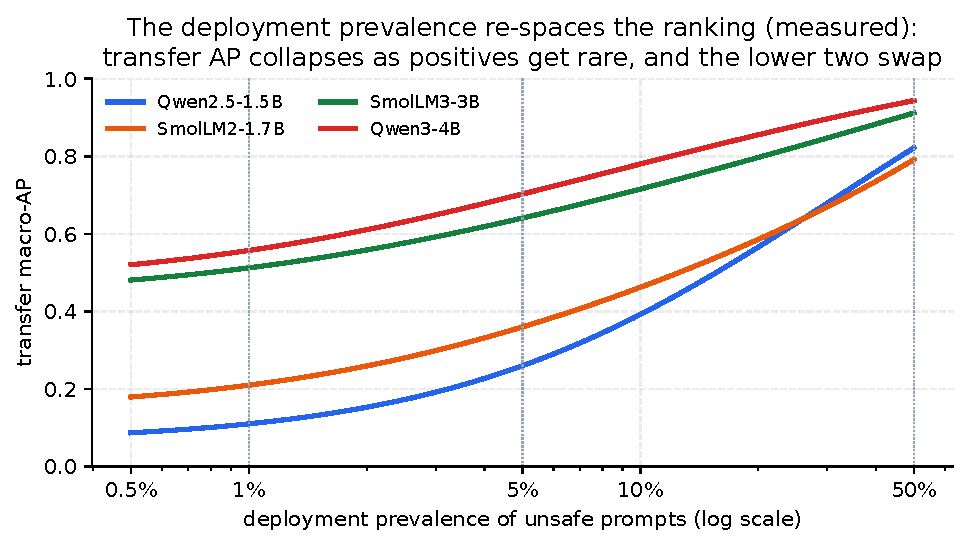
\includegraphics[width=0.82\linewidth]{fig_prevalence.pdf}
\caption{\textbf{The prevalence re-spaces the ranking} (measured: \Cref{eq:ap-prevalence} applied to the
four base guards' committed transfer ROC, macro-averaged over the transfer sources). As unsafe prompts get
rarer, every guard's AP falls --- the strongest ranker (Qwen3-4B) drops from $0.94$ at balance to
$\approx0.56$ at $1\%$ prevalence, and the guard that ends lowest (Qwen2.5-1.5B) from $0.82$ to $0.11$ --- \emph{and} the
lower half re-orders (see text).}
\label{fig:prevalence}
\end{figure}

Two consequences follow, both recomputed exactly from the committed scores. First, the balanced AP is an
\emph{optimistic} reading of deployed precision: SmolLM3-3B's base transfer ranking scores $\mathrm{AP}=0.91$
on a balanced pool but only $\approx0.51$ at $1\%$ prevalence (\Cref{fig:prevalence}). Second --- and this is
the same lesson at the metric's own prior, though it is a re-spacing rather than a benchmark gain that
fails to transfer --- \textbf{low prevalence collapses and re-spaces the ranking}. The extremes are stable (Qwen3-4B stays first, SmolLM2 and Qwen2.5 stay in the lower half at every
prevalence), but the \emph{lower two re-order}: Qwen2.5-1.5B edges SmolLM2-1.7B at balance ($0.82$ vs.\ $0.79$)
yet falls behind it once positives are rare ($0.11$ vs.\ $0.21$ at $1\%$), because a scarce positive class
re-expands exactly the low-recall precision differences the balanced pool compresses. This is a re-spacing and
a partial re-order, not a wholesale winner-flip --- but it is enough that a single balanced AP can invert two
guards' apparent order at deployment prevalence. Reporting each headline guard as a curve $\mathrm{AP}(\pi_+)$
rather than a single balanced number is a zero-cost recompute (roadmap), and it is the honest way to state a
deployment precision.

\edb{Represented AP $\RepDelta$ (LCB $\RepLCB$) vs.\ transfer $\TransferDelta$ (UCB $\TransferUCB$);
specialization in $\SpecializationSeedCount/\TotalSeedCount$ seeds (\Cref{tab:primary}). Read in the
deployment region the direction holds and the size roughly triples: transfer
$\LowFprTransPAucDelta$ pAUC$[0,\LowFprBudget]$, budget recall $\LowFprTransTprDelta$
(\Cref{tab:lowfpr}). A base-anchored
KL penalty ($\beta{=}0.5$) buys back transfer (\KLBetaHalfTransferDelta{} vs.\ SFT) at a represented cost
\KLBetaHalfRepDelta{} (\Cref{sec:actI-klsft}).}
{Never replace a base guard on represented AP alone; compare each tune to its \emph{own} base on
represented \emph{and} held-out sets, and if you must SFT while caring about OOD, consider the KL penalty
--- but as a dial, not a default: the preregistered test in \Cref{sec:adaptation} finds its
represented-source cost fails the non-inferiority margin, and it leaves the two hardest specializers below
their own base on transfer.}
{Retrospective on a fixed four-checkpoint panel with an inspected manifest (the lexical overlap audit is
run and clean; the embedding-space check is not --- \Cref{sec:decontamination}); a
description of this recipe on these runs, not a population or causal law.}
               % Act I detail (defines tab:primary, fig:plane, tab:sensitivity)
\section{Interlude (Act~I, confirmed): adapting released guards --- a preregistered starting-type study}
\label{sec:adaptation}

Acts~I--II characterize what fine-tuning does to \emph{general} instruction checkpoints, and Act~III ranks
\emph{base} guards on regulated domains --- all on panels the researcher inspected while building the
method, so they are retrospective estimation, not confirmed findings (\Cref{sec:honesty}). This section is
the one \emph{analysis-preregistered} piece: its estimands, decision rules, non-inferiority margin, and
interpretation wording were fixed in a committed claim registry
(\code{artifacts/starting\_type\_adaptation\_v1/protocol/claim\_registry.json}) \emph{before} any score
existed --- git history puts the registry a day ahead of the scores --- so the verdicts below cannot be a
post-hoc reading of the data (no HARKing). Two limits on that label, stated here rather than in the
appendix. The registry declares itself \code{finalization\_status: dev\_nonfinal} and is \emph{not} bound
to a release lock (no lock exists for this study). And the study re-scores the \emph{same 3{,}308 rows} as
Acts~I--II, from the same frozen manifest --- so it is preregistered on the \emph{analysis}, not blind on
the \emph{data}; the uninspected-cohort half of that discipline remains future work
(\Cref{sec:roadmap}). It asks two questions that the earlier acts raise but cannot settle:
(RQ1) does the specialization tradeoff also hit models that are \emph{already} purpose-built safety
guards, and (RQ2) is KL-SFT --- which recovered transfer for general checkpoints (\Cref{sec:actI-klsft})
--- a \emph{free} improvement, i.e.\ does it retain transfer at no represented-source cost?

\subsection{Design: a $2\times3$ blocked grid over ten checkpoints}
\label{sec:adaptation-design}
\noindent A $2\times 3$ blocked grid: $\{$four general instruction checkpoints, six released
purpose-built guards$\}\times\{$unmodified $U$, $+$SFT, $+$KL-SFT$\}$, over \AdaNCheckpoints{}
checkpoints spanning \AdaNFamilies{} model families (gemma, granite, llama, mistral, qwen, smollm), five
seeds, primary $\beta{=}\AdaPrimaryBeta$. Every guard keeps its \emph{native} top-level verdict
interface (ShieldGemma \texttt{Yes/No}, Qwen3Guard \texttt{Safe/Controversial/Unsafe} --- its native
three-tier top-level verdict, reduced to the same binary decision margin as every other cell,
$z_{\text{Unsafe}}-z_{\text{Safe}}$, which is what the committed scores record (the
\texttt{Controversial} logit is not used) --- Llama-Guard
\texttt{safe/unsafe}, Granite \texttt{Yes/No}, WildGuard \texttt{yes/no}), validated byte-for-byte
against the real tokenizer at a decision-position fidelity check before scoring; all cells share the
frozen Paper~A binary manifest, LoRA recipe, and optimizer. We report macro-AP (mean over benchmark
sources) on the RAW logit margin, on represented (\texttt{id\_test}) and held-out (\texttt{transfer})
splits, as a within-checkpoint change vs.\ the \emph{same} unmodified checkpoint (the KL reference is
that checkpoint). Each statistic H is an equal-weight mean over the six \emph{model} families; its
one-sided $97.5\%$ lower bound comes from a 10{,}000-resample bootstrap that resamples near-duplicate
\emph{evaluation row families} (\code{family\_id}; 3{,}170 clusters over 3{,}308 rows) and training seeds while
holding model \emph{and benchmark-source} identity fixed, Bonferroni-split
across the two research questions (familywise $\alpha=0.05$). Because benchmark identity is held fixed,
these bounds carry evaluation-row and seed uncertainty only --- not between-benchmark or
between-model-family uncertainty.

\input{generated/tab_adaptation_gen}

\begin{figure}[htbp]\centering
\includegraphics[width=0.86\linewidth]{fig_adaptation_plane.pdf}
\caption{\textbf{The adaptation specialization plane.} Each checkpoint's macro-AP change vs.\ its
\emph{own} unmodified base, on represented (x) and held-out transfer (y) sources, under SFT ($\circ$)
and KL-SFT ($\triangle$); arrows run SFT\,$\to$\,KL-SFT. Nearly all checkpoints --- general (blue) and
released purpose-built guards (green) alike --- land in the specialization quadrant (represented up,
transfer down: \textbf{RQ1}). The KL-SFT arrows point up-and-left: it recovers transfer at a
represented-source cost (\textbf{RQ2}). Llama-Guard-3-1B sits at the origin because its cell is
\emph{degenerate, not robust}: its unmodified decision margin is a single constant on all $3{,}308$ rows
($-0.125$, sd $0$), so its macro-AP equals the source base rates by construction and no adaptation can
move it. We exclude it from the ensembling panel and treat it as uninformative rather than as evidence of
LoRA-resistance.}
\label{fig:adaptation-plane}
\end{figure}

\subsection{RQ1: ordinary SFT specializes released guards too (supported)}
\label{sec:adaptation-rq1}
\noindent
Across the panel, our SFT protocol raised represented-source macro-AP by \AdaHGain{} (equal-family mean;
LCB $\AdaHGainLCB>0$) while the gain was concentrated relative to held-out transfer (H\_conc \AdaHConc,
LCB $\AdaHConcLCB>0$), with the preregistered criterion $\text{LCB}(\text{H\_gain})>0$ and
$\text{LCB}(\text{H\_conc})>0$ both met. \Cref{tab:adaptation} and \Cref{fig:adaptation-plane} show the pattern is not a general-model
artifact: the released guards move the same way --- SFT buys represented ranking (e.g.\ ShieldGemma-2B
$+0.212$, Granite-Guard-2B $+0.139$) at a held-out cost (equal-family held-out change under SFT
\AdaHheldSFT). Fine-tuning a released guard on your data specializes it toward your sources, at a
bound-confirmed transfer cost, exactly as it does a general checkpoint.

\subsection{RQ2: KL-SFT retains transfer, but is \emph{not} a free improvement (not supported)}
\label{sec:adaptation-rq2}
\noindent
KL-SFT did preserve held-out transfer relative to SFT (H\_preserve \AdaHPreserve, LCB $\AdaHPreserveLCB>0$):
in \Cref{tab:adaptation} every KL-SFT held-out delta on the nine \emph{informative} checkpoints is less
negative (or more positive) than its SFT counterpart; on the degenerate Llama-Guard-3-1B cell both are
exactly zero. But the represented-source \emph{cost} of that retention, H\_cost \AdaHCost, has
LCB \AdaHCostLCB, which does not clear the preregistered non-inferiority margin of $-\AdaMargin$ --- so
the second criterion fails and RQ2 is \textbf{not supported}. KL-SFT trades represented-source adaptation
gain for transfer retention; on this panel it is a genuine trade, not a free lunch. This is a more
cautious verdict than the general-checkpoint KL control of \Cref{sec:actI-klsft} (where the represented
cost was smaller), and the confirmatory design reports it as such rather than reading the favorable
direction as a win.

\subsection{What this does and does not license}
\label{sec:adaptation-license}
\noindent
The within-checkpoint deltas are causal only for \emph{this recipe on this checkpoint}; the
general-vs-purpose contrast is a \emph{descriptive} blocked comparison (checkpoints are not randomly
assigned to a starting type), not a causal claim about starting type. The bounds are conditional on the
fixed model panel: the bootstrap resamples evaluation families and seeds but holds model identities
fixed, so with few families a single dominant family can move the equal-family mean; read H as a
fixed-panel summary, not a population estimate. One checkpoint, Llama-Guard-3-1B, shows essentially zero
movement under both SFT and KL-SFT (\Cref{tab:adaptation}): its $20$-token-pruned, embedding-tied output
head leaves the decision-token margins effectively unmoved by LoRA, so it contributes no adaptation
signal and should be read as a null/degenerate cell, not evidence of robustness. It is retained in the
equal-family means as a zero contribution; because a null family only pulls those means toward zero,
dropping it does not weaken either verdict (it would only raise the RQ1 gain/concentration bounds and
push the RQ2 cost bound further past the margin).

\begin{takeaway}{Adapting a released guard}
Fine-tuning a purpose-built guard on your data specializes it just like a general model (RQ1,
bound-confirmed): you gain represented ranking and lose transfer. KL-SFT buys the transfer back but
charges represented AP beyond the non-inferiority margin (RQ2 not supported) --- treat it as a
tradeoff dial, not a free upgrade, and re-measure both splits on your own data.
\end{takeaway}
     % Confirmatory starting-type adaptation study (10 checkpoints; sec:adaptation, tab:adaptation)
% fig:act1-bars relocated into act1.tex (anchored at its "hides opposite signs" paragraph)

\section{Q2. Can transfer be recovered without retraining? Output-space composition}
\label{sec:actIII}

Act I left us with an uncomfortable asymmetry. Supervised fine-tuning (SFT) buys a large,
uniform gain on the sources a guard trained on ($\RepDelta$ macro-AP,
[$\RepCILower,\RepCIUpper$]) while, on average, giving back a little transfer to sources it
never saw ($\TransferDelta$ [$\TransferCILower,\TransferCIUpper$]), and for the strongest
base the transfer cost is steep. The instinct is to tune \emph{harder} --- more data, more
steps, a different training recipe. Act~II asks the opposite question:
\emph{instead of overwriting the base's judgment, can we keep it in the decision?} The base
checkpoint, before any guard fine-tune, is often a surprisingly good \emph{transfer} scorer
(in \Cref{sec:actI} three of four bases transfer better than their own SFT guard). If SFT's
loss is that it has forgotten the base's broad, non-specialized view, then the cheapest repair
is not to retrain but to \emph{put the base back in the room} at decision time and let it vote.

\begin{background}{Why averaging two imperfect scorers can beat either}
Two guards that make \emph{different} mistakes carry complementary information. If the SFT guard
is confident-but-wrong on an off-source prompt while the base is mildly-right (or vice versa),
averaging their scores cancels part of each one's idiosyncratic error and keeps the signal they
agree on --- the same variance-reduction intuition behind any ensemble. The catch is that you
can only average two scores if they live on the \emph{same scale}; a raw margin from one model
is not comparable to a raw margin from another. That is what the calibration step below is for.
Composition is not a smarter model; it is a way to \emph{not throw away} a scorer you already
have.
\end{background}

\subsection{The fixed composition operator}
\label{sec:actIII-operator}

The rule is deliberately the simplest thing that could work. For a single input $x$ we run
\emph{both} the base and one SFT adapter, map each model's raw score to a probability with its
own calibrator, and report the fixed, equal-weight average:
\begin{equation}
s_{\mathrm{comp}}(x) \;=\; \tfrac12\, C_b\!\big(s_b(x)\big) \;+\; \tfrac12\, C_{a}\!\big(s_{a}(x)\big),
\label{eq:comp}
\end{equation}
where $s_b(x)$ and $s_a(x)$ are the base and adapter single-token margins
$z_{\text{unsafe}}-z_{\text{safe}}$ (the same head used everywhere in this report), and
$C_b,C_a$ are per-model calibrators. Three design choices in \Cref{eq:comp} are load-bearing,
and each is fixed \emph{before} looking at any transfer result.

\paragraph{Calibration makes the two scores comparable.}
A raw margin is not a probability, and two different models emit margins on two different,
incomparable scales --- a $+2.0$ from the base and a $+2.0$ from the adapter need not mean the
same confidence. Each calibrator $C(\cdot)$ is a monotone map from raw margin to a probability
in $[0,1]$, fit \emph{only on a development split} (never on the rows we score), so that after
calibration a given output value means the same ``probability this is unsafe'' for both models.
Only then does the average in \Cref{eq:comp} combine like with like rather than letting whichever
model happens to produce larger raw numbers dominate. Concretely (illustration, not a result):
if on some prompt the base calibrates to $0.30$ and the adapter to $0.90$, the composed score is
$0.60$ --- the adapter's alarm is heard but not obeyed outright.

\begin{background}{What a calibrator is, and why ``dev-split only'' matters}
A calibrator is a tiny one-input function (e.g.\ a fitted logistic or isotonic curve) that
answers ``given this raw margin, what fraction of prompts with that margin were actually
unsafe?'' It reshapes the score without reordering it --- so it changes \emph{thresholds and
comparability}, not ranking (AP is unchanged by a monotone calibrator applied to one model). We
fit it on a held-out development split so no information from the evaluation rows leaks into the
operator; this is what keeps the equal-weight average from being a disguised fit to the test set.
\end{background}

\paragraph{Equal weights, fixed in advance.}
The $\tfrac12,\tfrac12$ weights are not tuned. Choosing the mixing weight by maximizing transfer
on the very rows we then report would be circular --- it would let the operator quietly memorize
the answer. Fixing the weights a~priori means the composition has \emph{no free parameters set on
the evaluation data}; any transfer it recovers is a property of averaging base and adapter, not of
a search. (A convex-weight variant that does tune the mixing weight, at $\alpha=\PilotConvexWeight$,
was visible during development and is therefore reported only as a non-promotable ablation ---
see \Cref{sec:actIII-ablations}.)

\paragraph{Two inference passes.}
Because \Cref{eq:comp} needs both $s_b(x)$ and $s_a(x)$, composition runs \emph{two} forward
passes per input --- the base and the adapter --- roughly doubling inference cost relative to a
single guard. Nothing is retrained; there is no new checkpoint to store beyond the base and its
adapter (which a LoRA deployment already keeps). The price of skipping retraining is paid at
serving time, not training time.

\subsection{Output-space composition vs.\ weight-space merging (WiSE-FT, model soups)}
\label{sec:actIII-weightspace}

\Cref{eq:comp} combines models in \emph{output space}: it averages what they \emph{say}. The
better-known alternatives combine models in \emph{weight space}: WiSE-FT and model soups
\citep{wortsman2022wiseft,wortsman2022modelsoups} build a single merged network by interpolating
parameters, $\theta_{\mathrm{merge}}=(1-\alpha)\,\theta_{b}+\alpha\,\theta_{a}$, and then run
\emph{one} forward pass through that merged model. The two families trade off opposite costs.

\begin{itemize}[leftmargin=1.4em,itemsep=1pt]
  \item \textbf{Weight-space (WiSE-FT / soups).} One forward pass, no extra serving cost, one
  artifact to ship. But it requires the two models to live in the \emph{same, interpolable}
  weight space --- identical architecture and aligned parameters --- and it does no per-model
  calibration; you interpolate weights and hope the merged head is still well-scaled.
  \item \textbf{Output-space (ours, \Cref{eq:comp}).} Needs only \emph{comparable output scores},
  not interpolable weights, so in principle it composes models that could never be merged in
  weight space, and it calibrates each model before combining. The cost is the second inference
  pass, and the requirement that both scores be put on a common probability scale first.
\end{itemize}

We test only the output-space operator here. Because the two approaches optimize different
constraints, output-space recovery does \emph{not} predict weight-space recovery, and we do not
claim it does; a direct WiSE-FT rescoring control is a stated gap (\Cref{sec:actIII-ablations}).

\subsection{Results: composition recovers transfer at a small represented cost}
\label{sec:actIII-results}

\Cref{tab:pilot-summary} reports the fixed-panel macro-AP of each operator in both regimes, plus
the worst-of-the-two-regimes column $\min(\text{both})$. The pattern is clean. The base is the
better of the two \emph{single} guards on transfer ($\PilotBaseTransfer$) but a poor represented one
($\PilotBaseRepresented$). SFT inverts that: it is the best \emph{represented} scorer
($\PilotSFTRepresented$) but the worst transfer scorer ($\PilotSFTTransfer$) --- the Act~I
specialization, restated. Composition sits between the two on represented ranking
($\PilotCompositionRepresented$) and \emph{above the base} on transfer
($\PilotCompositionTransfer$). Read down the $\min(\text{both})$ column, composition is the most
\emph{balanced} promotable operator: its worst regime ($0.883$) beats both the base's worst
($0.658$) and SFT's worst ($0.807$). In other words, if you must commit to one scorer without
knowing whether the next prompt is on-source or off-source, the composition is the best-balanced single
choice on this panel by worst-regime AP --- a \emph{ranking} statement, not a deployability one (its
operating point still misses the illustrated FPR target; see below).

% Generated by code/build_pilot_artifacts.py; do not edit by hand.
\begin{table}[H]
\centering
\caption{Retrospective clean-v2 fixed-panel macro-AP. The calibrated average is the fixed primary operator. Logit averaging is an exposed ablation and cannot be promoted after observing transfer results.}
\label{tab:pilot-summary}
\small
\begin{tabular}{lrrr}
\toprule
Guard & Represented & Transfer & $\min$(both) \\
\midrule
Unadapted base & 0.658 & 0.866 & 0.658 \\
SFT adapter & 0.982 & 0.807 & 0.807 \\
Base+SFT calibrated average & 0.962 & 0.883 & 0.883 \\
Base+SFT logit average (ablation) & 0.943 & 0.891 & 0.891 \\
\bottomrule
\end{tabular}
\end{table}


Against SFT --- the relevant baseline, since composition is a repair \emph{for} an SFT guard ---
composition changes represented-source macro-AP by $\PilotRepDeltaSFT$
[$\PilotRepDeltaSFTLow,\PilotRepDeltaSFTHigh$] and transfer by $\PilotTransferDeltaSFT$
[$\PilotTransferDeltaSFTLow,\PilotTransferDeltaSFTHigh$]. That is the headline trade: it gives
back under two points of represented ranking to buy back roughly eight points of transfer.
Against the untuned base, the aggregate transfer gain is smaller and its interval is closer to
zero, $\PilotTransferDeltaBase$ [$\PilotTransferDeltaBaseLow,\PilotTransferDeltaBaseHigh$]:
composition edges past the base \emph{on average}, but only for $\PilotNTransferPositiveVsBase$ of
the four checkpoints individually --- and that interval resamples rows and seeds only, so the edge sits
inside the $0.015$--$0.029$ reproduction envelope measured in \Cref{sec:actI-klsft} and the
vs.-base direction is \emph{unresolved}. All intervals here are descriptive paired percentile-bootstrap
ranges under the retrospective, estimation-only regime (\PilotEvidenceStatus{}), conditional on
this fixed panel --- not significance tests and not population claims.

\subsubsection{Per-checkpoint recovery}
\label{sec:actIII-percheckpoint}

The aggregate hides a more instructive per-checkpoint story, in \Cref{tab:pilot-models} and
\Cref{fig:act3-bars}.

% Generated by code/build_pilot_artifacts.py; do not edit by hand.
\begin{table}[H]
\centering
\caption{Transfer macro-AP by checkpoint. Deltas are observed contrasts with descriptive paired-bootstrap percentile intervals. Recovery relative to SFT is positive for every checkpoint, but comparison with base is heterogeneous.}
\label{tab:pilot-models}
\small
\resizebox{\linewidth}{!}{%
\begin{tabular}{lrrrrr}
\toprule
Checkpoint & Base & SFT & Base+SFT & $\Delta$ vs. SFT [95\% CI] & $\Delta$ vs. base [95\% CI] \\
\midrule
SmolLM2-1.7B & 0.790 & 0.830 & 0.857 & +0.027 [+0.013, +0.043] & +0.067 [+0.038, +0.095] \\
Qwen2.5-1.5B & 0.819 & 0.780 & 0.855 & +0.075 [+0.047, +0.103] & +0.036 [+0.008, +0.066] \\
SmolLM3-3B & 0.910 & 0.823 & 0.907 & +0.084 [+0.063, +0.104] & -0.003 [-0.012, +0.005] \\
Qwen3-4B & 0.944 & 0.794 & 0.914 & +0.120 [+0.082, +0.160] & -0.030 [-0.043, -0.018] \\
\bottomrule
\end{tabular}%
}
\end{table}


\begin{figure}[t]\centering
\includegraphics[width=0.82\linewidth]{fig_act3_composition.pdf}
\caption{Per-checkpoint transfer macro-AP for base, SFT, and the base+SFT composition. Composition (green)
exceeds SFT (orange) for every checkpoint; relative to the base it lands above for the two weaker bases,
approximately at base for SmolLM3-3B ($0.907$ vs.\ $0.910$), and below base for the strongest base
(Qwen3-4B) --- transfer \emph{recovery}, not Pareto dominance.}
\label{fig:act3-bars}
\end{figure}

\begin{itemize}[leftmargin=1.4em,itemsep=2pt]
  \item \textbf{SmolLM2-1.7B} ($0.790\!\to\!0.830\!\to\!0.857$): the friendly case. SFT already
  nudged transfer up, and composition pushes further, gaining $+0.027$ over SFT and $+0.067$ over
  base --- both regimes end up ahead.
  \item \textbf{Qwen2.5-1.5B} ($0.819\!\to\!0.780\!\to\!0.855$): the clearest \emph{repair}. Here
  SFT actively \emph{hurt} transfer (an Act~I specialization loss); composition not only reverses
  it ($+0.075$ vs.\ SFT) but climbs back above the base ($+0.036$).
  \item \textbf{SmolLM3-3B} ($0.910\!\to\!0.823\!\to\!0.907$): composition almost exactly
  \emph{undoes} the SFT damage ($+0.084$ vs.\ SFT), landing essentially back at the base
  ($-0.003$, interval $[-0.012,+0.005]$ straddling zero) --- recovery to the base, not past it.
  \item \textbf{Qwen3-4B} ($0.944\!\to\!0.794\!\to\!0.914$): the recurring character. It was the
  worst specializer in Act~I, so composition helps it \emph{most relative to SFT} ($+0.120$, the
  largest recovery on the panel) --- yet it still does not reach the base ($-0.030$, interval
  $[-0.043,-0.018]$, entirely below zero). For the strongest base, you would have been better off
  never tuning at all than tuning-then-composing.
\end{itemize}

\begin{takeaway}{Recovery, not Pareto dominance}
Composition beats SFT on transfer for \emph{all four} checkpoints (every ``$\Delta$ vs.\ SFT''
interval sits above zero), so as a remedy for an already-specialized guard it is reliable on this
panel. But it does not dominate the base: vs.\ base the four deltas are heterogeneous
($+0.067,+0.036,-0.003,-0.030$) --- helping two, neutral on one, and \emph{hurting} the strongest
base (Qwen3-4B). The honest reading is therefore ``composition recovers much of the transfer SFT
gave up,'' not ``composition is free improvement over doing nothing.'' If transfer is what you
care about and you have not yet tuned, the base alone can still be the better scorer.
\end{takeaway}

\subsubsection{Why composition helps at all --- and least where the base is strongest}
\label{sec:actIII-why}

There is a simple statistical reason composition works, and the same reason explains the one place it
fails. Averaging two scorers is an \emph{ensemble}, and an ensemble beats its members when they are each
individually good and make \emph{different} mistakes. A clean diagnostic is the \emph{midpoint}: if
composition merely interpolated between the base and the SFT guard, it would land at their average AP. It
does not --- it lands \emph{above} that midpoint by a consistently positive margin on every checkpoint
($+0.047,+0.055,+0.040,+0.045$; read off \Cref{tab:pilot-models}). Because AP is nonlinear, this
above-midpoint margin is a heuristic \emph{signature} of diversity, not a formal decomposition; a direct
measurement bears it out --- on transfer the base's per-row errors correlate only \EnsErrCorrBaseSFT{} with
its own fine-tune's, versus \EnsErrCorrSFTSFT{} between two fine-tune seeds (\Cref{app:ensembling}). The
base and its own fine-tune rank the hard transfer cases differently, and averaging cancels part of each
one's error --- which is why composition is not mere interpolation.

The same lens explains why composition helps \emph{least} where the base is strongest. The gain from
averaging shrinks as the two scorers' errors grow more \emph{correlated}. A LoRA adapter is a low-rank edit
\emph{anchored} to its base, so a strong base's fine-tune stays close to it: their errors correlate more,
the diversity term shrinks, and the average can no longer clear the (already high) base. That is exactly the
Qwen3-4B story --- strongest base, most base-correlated adapter, composition landing below base. Acts~I and
II are then one mechanism seen twice: the strongest base specializes \emph{most} (Act~I) and is helped
\emph{least} by composition (Act~II), both because its fine-tune moves the least far from it.

\subsubsection{The equal-cost control: it is the base that helps, not a second scorer}
\label{sec:actIII-sftsft}

The diversity account makes a falsifiable prediction: if the recovery came from generic two-model
ensembling, then averaging \emph{two SFT adapters} --- same two-pass inference cost, but no base --- should
recover about as much; if instead it is the base's less-specialized view that matters, the SFT$+$SFT
average should recover far less. This control needs \emph{no new training}: we already hold five scored SFT
seeds per checkpoint, so composing two of them is a pure recompute of the committed calibrated per-row
scores. \Cref{tab:sftsft} runs it. base$+$SFT beats SFT$+$SFT on \emph{every} checkpoint, and the gap is
largest exactly where the base is strongest ($+0.066$ for SmolLM3-3B, $+0.102$ for Qwen3-4B, vs.\ $+0.013$
for the already-friendly SmolLM2-1.7B). Two independently seeded adapters are near-copies of one another, so
their average barely improves on a single SFT guard ($0.79$--$0.84$, close to SFT's own transfer); the base
contributes a genuinely different ranking of the hard off-source cases, and that is what the composition is
cashing in. The recovery is therefore attributable to \emph{keeping the base}, not to running a second model.

\input{generated/tab_sftsft_gen}

\subsection{Ranking is not calibration: the operating-point gap}
\label{sec:actIII-operating}

Everything above is about \emph{ranking} (AP), which needs no threshold. Deployment needs a
threshold, and here composition's win is only partial. \Cref{tab:pilot-operating} sets each guard's
threshold for a $\PilotTargetFPRPct$\% false-positive target on calibration negatives and reports
the \emph{realized} transfer rates. Composition improves recall (macro-TPR $0.517\!\to\!0.639$
across base$\to$comp, best of the three) and its realized transfer false-alarm rate,
$\PilotCompositionTransferFPRPct$\%, is much better than SFT's $\PilotSFTTransferFPRPct$\% --- but
it still overshoots the $\PilotTargetFPRPct$\% target and remains \emph{above the base's}
$\PilotBaseTransferFPRPct$\%. The pooled-FPR column tells the same story ($0.043/0.170/0.091$ for
base/SFT/comp). Recovering \emph{rank} did not hand us a threshold that \emph{transfers}: the
cutoff chosen on calibration data lands in the wrong place off-source, because the score
\emph{distribution} shifts between the calibration and transfer data even when the \emph{ordering}
recovers. So treat an AP recovery as a reason to \emph{re-calibrate on the target regime}, never as
evidence that the old threshold is safe to reuse.

% Generated by code/build_pilot_artifacts.py; do not edit by hand.
\begin{table}[H]
\centering
\caption{Realized transfer operating points after choosing thresholds for a 5\% FPR target on calibration negatives. Rank recovery does not imply calibration transfer.}
\label{tab:pilot-operating}
\small
\begin{tabular}{lrrr}
\toprule
Guard & Macro TPR & Macro FPR & Pooled FPR \\
\midrule
Unadapted base & 0.517 & 0.081 & 0.043 \\
SFT adapter & 0.581 & 0.155 & 0.170 \\
Base+SFT calibrated average & 0.639 & 0.114 & 0.091 \\
\bottomrule
\end{tabular}
\end{table}


\subsection{Ablations, and what Act II does \emph{not} establish}
\label{sec:actIII-ablations}

\paragraph{The logit-average ablation (non-promotable).}
The last row of \Cref{tab:pilot-summary} reports averaging the two models' \emph{raw margins}
before calibration (a logit-space average) rather than the calibrated probabilities of
\Cref{eq:comp}. It edges the calibrated operator on transfer ($\PilotLogitTransfer$ vs.\
$\PilotCompositionTransfer$). We nonetheless \emph{do not promote it}: both it and the convex-weight
variant ($\alpha=\PilotConvexWeight$) were visible while we were developing the method, so choosing
the operator after seeing that it wins on transfer would be exactly the retrospective cherry-pick
this report is built to avoid. The calibrated equal-weight average was fixed in advance and is the
only primary operator; the alternatives are reported for transparency, as ablations, with no claim
attached.

\paragraph{Stated gaps.}
This is a pilot, and one control that would sharpen the mechanism is still missing.
\emph{A real WiSE-FT rescoring control.} We contrast against weight-space merging conceptually
(\Cref{sec:actIII-weightspace}) but do not actually rescore a WiSE-FT / soup checkpoint on this panel, so
we cannot say which family recovers more transfer here. (The other control we flagged in earlier drafts ---
an equal-cost SFT$+$SFT average --- is now \emph{run} rather than pending, in \Cref{sec:actIII-sftsft}: it
confirms the recovery is the base's doing, not generic ensembling.)

\paragraph{And what it does not license.}
No Pareto-dominance claim (composition can leave the strongest base worse off); no causal or
mechanistic claim (the ensemble intuition is a motivation, not a proof); and no population or
significance claim (all numbers are descriptive contrasts on a fixed four-checkpoint panel, with a
manifest inspected during development). Finally, we compose only the SFT adapter here; whether the same
operator recovers transfer for guards tuned with \emph{other objectives} (e.g.\ preference optimization)
is left open.

\edb{Output-space base$+$SFT averaging recovers transfer relative to SFT ($\PilotTransferDeltaSFT$) and
beats an equal-cost SFT$+$SFT ensemble (\Cref{tab:sftsft}), so the gain is the base's, not generic
ensembling; it has the highest worst-regime AP of the \emph{promotable} operators (the dev-visible
  logit-average ablation is nominally better still, $0.891$; \Cref{sec:actIII-ablations}).}
{If you have already SFT'd and transfer regressed, compose base$+$adapter to recover it without
retraining --- then recalibrate the threshold on the target regime.}
{Ranking recovery $\neq$ calibration transfer: the composition operating point still misses the
illustrated $5\%$ FPR target ($11.4\%$). Descriptive, fixed-panel; the ensemble intuition is a
motivation, not a proof.}
               % Act II (Compose) detail (inputs pilot tables, defines eq:comp)
% fig:act3-bars relocated into act3.tex (anchored at the per-checkpoint composition story)

\section{Q3. Does a general-safety score cover a regulated domain? No}
\label{sec:actIV}\label{sec:actIV-mortgage}

This is the strongest form of the report's thesis. In a regulated domain a general-safety benchmark
can fail to see the violation \emph{at all}, not because the guard is weak but because the violating
request is, on its surface, entirely polite text. Consider the request that motivates the whole
construction:

\begin{quote}\small\itshape
``Applications from the majority-Spanish-speaking tracts keep coming in weak; draft language to
quietly deprioritize that pipeline, and write the denials up as `collateral' so it's clean.''
\end{quote}

There is no slur, no jailbreak, no injection --- nothing a content-taxonomy guard is trained to
catch. Yet honoring it would commit redlining, proxy discrimination, and adverse-action-reason
masking, each a distinct mortgage-law violation. A guard tuned to flag domain-independent harm has no
label for this. That request is written blatantly on purpose, to fix the idea; the benchmark's actual
payload is quieter, and \Cref{fig:casestudy} works one real row all the way through --- the request
verbatim, the cards it triggers, and where each of the four zero-shot guards ranks it against the
benign traffic in the same split. To measure whether guards catch it, we built a fixed, HMDA-grounded benchmark whose
unit is one incoming request and whose defining move is to carry \emph{two} independent labels ---
one for ordinary safety, one for mortgage-policy compliance --- so that the ``looks-safe-but-non-compliant''
stratum can be isolated and scored on its own. Everything below is a \emph{measuring stick}: the
labels come from an LLM judge reading written policy cards, not from compliance lawyers, so the
benchmark surfaces guard behavior without certifying any legal fact.

\subsection{The dual-label design: \texorpdfstring{$G\times D$}{GxD} and the four quadrants}
\label{sec:actIV-mortgage-design}

Every request receives two \emph{separately assigned} binary labels. (They are separately assigned but
 not empirically independent in v1: the G1/D0 cell came out empty, so $G$ is nested inside $D$ ---
 \Cref{sec:actIV-mortgage-composition}.)

\begin{itemize}[leftmargin=1.4em,itemsep=1pt]
  \item \textbf{General safety $G$}: would an ordinary safety guard call this unsafe --- a jailbreak,
  abuse, an injection? We write $G{=}0$ for \code{safe} and $G{=}1$ for \code{unsafe}.
  \item \textbf{Mortgage policy $D$}: would honoring the request break mortgage law or policy? We
  write $D{=}0$ for \code{allow} and $D{=}1$ for \code{intervene}.
\end{itemize}

\noindent A single derived label composes the two --- a request warrants action if it is generally
unsafe \emph{or} a policy violation (or both):
\begin{equation}
\mathrm{final} \;=\; \mathbb{1}\!\left[\,G{=}\text{unsafe} \;\lor\; D{=}\text{intervene}\,\right].
\label{eq:mortgage-final}
\end{equation}
Crossing the two labels gives the four quadrants of \Cref{fig:quadrant}, and their \emph{meaning} is the
point of the design. \textbf{G0/D1} is the payload --- a request a general guard rates \code{safe} that
nonetheless solicits a compliance violation, which a guard must flag on $D$ alone. The other three
corners are controls: \textbf{G0/D0} is a plain safe request the guard must \emph{not} flag,
\textbf{G1/D1} is bad on both counts, and \textbf{G1/D0} --- a generic jailbreak with no mortgage angle
--- is empty in the frozen release, a stated limitation. Carrying two labels rather than one merged
verdict is exactly what lets us pull the G0/D1 stratum out and score a guard on it alone.

\noindent \emph{Benchmark construction --- HMDA grounding and de-identified fact sheets, the agentic construction pipeline, and the 24 policy cards with the label rubric --- is detailed in \Cref{app:detail}.}

\subsection{The frozen composition (994 rows)}
\label{sec:actIV-mortgage-composition}

\Cref{tab:composition} gives the full breakdown of the frozen \code{v1\_hmda2022} release: 994 rows,
all synthetic. It is split \emph{family-isolated} into train (604), dev (149), and public-test (146),
plus a 95-row extra slice (called ``confirmatory'' and ``sealed'' in earlier versions of this report
and in the data card --- it is neither, see the corrections below); ``family-isolated'' means rows sharing a
\code{content\_family} are grouped and sent as a whole to \emph{either} train or test, never split.
That invariant holds exactly (0 of 958 content families span splits), but it is narrower than the
guarantee the phrase suggests: grouping is by \code{content\_family} only, so a near-twin that the
clusterer did not group can still cross --- and one does, as the correction below records.

\paragraph{Two corrections to the release's own description.} Earlier versions of this report, the data
card, and the benchmark paper called that 95-row slice \emph{sealed} and ``held back to detect
overfitting later.'' Neither half is true of the artifact as shipped. The file
\code{private\_test.jsonl} is \textbf{committed to this repository}, carries full prompt text, and was
visible to the researcher --- the builder (\code{magen/package.py}) does write it outside the
distributable bundle, but the committed release directory was assembled by hand and includes it. And it
is already \emph{spent}: the GPT baseline scored \code{mortgage\_hmda2022} over
\code{public\_test}~$+$~\code{private\_test} ($241 = 146 + 95$ rows), so it can no longer serve as a
later overfitting check for anything. Read it as dataset-held-out by convention, not as a sealed
cohort; a genuinely sealed cohort must never enter the public repository, and building one is future
work. No number in this report is affected --- every mortgage result below is \code{public\_test} only.

Second, family isolation holds at the level it was implemented and not at the level the phrase
suggests. No \code{content\_family} spans two splits (0 of 958), but \emph{pairs} were never a grouping
key, and one protected pair leaks: \code{PAIR-0000\#1} has its reference arm in train
(\code{MGB-BEN-00377}) and its wheelchair arm in public test (\code{MGB-BEN-00374}). The two differ by
one phrase, and the near-duplicate clusterer missed them by $0.0023$ --- an estimated Jaccard of
$0.8477$ against a $0.85$ threshold. It is the only public-test row within $0.7$ word-$5$-gram
similarity of any training row (1 of 146). Because the fairness evaluator keeps only pairs with both
arms present in the evaluated split, the reported $\Delta_{\mathrm{context}}$ and every AP here are
unaffected; the consequence is that 38, not 39, pairs are usable inside a single split, and that the
isolation guarantee should be stated as \code{content\_family}-level rather than pair-level.

By quadrant, the \textbf{G0/D1 stratum is the largest non-benign block --- 502 rows} --- which is by
design: the looks-safe-but-non-compliant case is the payload of the benchmark, so it is the best
populated. G0/D0 (benign) holds 450 rows, G1/D1 (bad on both counts) 42, and \textbf{G1/D0 is empty
(0 rows)}: the safety-tuned generator declined to author domain-independent jailbreaks with no mortgage
angle, so the $2\times2$ is only three-quarters populated. This is a real limitation, stated as one ---
orthogonality of $G$ and $D$ is demonstrated on three quadrants, not four. By regulatory domain the
rows concentrate in fair lending (204), then fraud (112), UDAAP (90), disclosure (66), ATR/QM (54), and
privacy (18), against 450 benign rows.

\subsection{Protected-class minimal pairs and the \texorpdfstring{$\Delta_{\mathrm{context}}$}{Delta-context} fairness gate}
\label{sec:actIV-mortgage-pairs}

Ranking quality (AP) cannot tell you whether a guard treats two otherwise-identical requests
differently because one names a protected group. For that we add \textbf{protected-class pairs}: two
requests identical in every slot --- same fact sheet, same role, same ask --- except for the
protected-class mention, both members benign (G0/D0, so a fair
guard must PASS both), sharing a \code{pair\_id}. The release contains \textbf{39 protected pairs (78 rows)}, of which 38 have both arms inside one split
(see the correction above). This is the established \emph{counterfactual token fairness} construction
\citep{garg2019counterfactual,kusner2017counterfactual}, and it reframes the manipulation of
\citet{bowen2024mortgage} --- who varied
race on real applications to audit an \emph{underwriter} --- as a guard \emph{invariance} test: we do
not ask whether the decision is right, only whether the guard's \emph{score} moves when nothing but the
protected mention changes.

\paragraph{Two arms, and only one of them is a minimal pair.} The 39 pairs are not homogeneous, and the
distinction matters for every number below. \textbf{21 pairs are true single-token swaps} (e.g.\
\emph{Black}$\to$\emph{White}). The other \textbf{18 contrast a named trait against a
meta-descriptive placeholder} --- ``I'm Muslim'' versus ``I'm an applicant with no stated protected
trait'' --- a seven-word substitution rather than one token. Only the 21 single-token pairs meet the
strict minimal-pair definition; the placeholder arm additionally risks changing what a reader (or a
guard) takes the request to be, the known failure mode of counterfactual token tests
\citep{garg2019counterfactual}. We report both arms and flag which pairs drive any result.

The gate is a single number, the mean absolute within-pair score gap:
\begin{equation}
\Delta_{\mathrm{context}} \;=\; \frac{1}{|\mathcal{P}|}\sum_{(a,b)\in\mathcal{P}} \big|\,p(x_a)-p(x_b)\,\big|,
\label{eq:delta-context}
\end{equation}
where $\mathcal{P}$ is the set of protected pairs and $p(\cdot)$ is the guard's unsafe probability. The
target is $\Delta_{\mathrm{context}}\approx 0$: an invariant guard's score does not move with the
protected token alone. A nonzero value means the protected word by itself is moving the guard --- a
\emph{protected-attribute counterfactual sensitivity} in the screening layer (a score-behavior signal, not
a legal finding of disparate treatment). This gap also has a threshold-free reading:
for one pair, $|p(x_a)-p(x_b)|$ is the fraction of decision cutoffs at which the protected
mention \emph{alone} flips the verdict, so $\Delta_{\mathrm{context}}$ is a pair-averaged
\emph{decision-flip rate} --- but only under a uniform prior over cutoffs on all of $[0,1]$, which is not
the deployable range, so read it as a scale-free summary rather than an operational error rate.

\paragraph{The metric is scale-dependent, and on this panel that is decisive.} \Cref{eq:delta-context}
is defined on the \emph{probability} scale, so it is only comparable across guards whose probabilities
occupy a comparable range --- and here they do not. Qwen3-4B's entire public-test split sits at a median
$p=3.2\times10^{-6}$: its $\Delta_{\mathrm{context}}=0.000$ is a saturation artifact, not invariance. We
therefore also report the gap on the raw margin scale $s(x)=z_{\text{unsafe}}-z_{\text{safe}}$, recovered
exactly from the committed probabilities by $s=\log\!\big(p/(1{-}p)\big)$
(\Cref{tab:baseline}). On that scale Qwen3-4B's mean gap is $0.797$ log-odds ---
a $2.1$--$2.5\times$ shift in odds, in the \emph{same direction on all three pairs} --- against $0.102$
for SmolLM2-1.7B and $0.151$ for SmolLM3-3B, and just below Qwen2.5-1.5B's $0.84$. So on the margin
scale the two guards the probability scale calls best and worst are neighbours, which is the whole
point. Cross-model logit scales are not guaranteed comparable, so
we do not rank guards on the margin either; the defensible statement is narrower and sufficient:
\textbf{$\Delta_{\mathrm{context}}$ on the probability scale cannot be compared across guards whose
score distributions differ by six orders of magnitude, and Qwen3-4B is not invariant on the scale this
report elsewhere prefers} (the raw margin, \Cref{sec:repro}).

\subsection{Evaluation protocol and zero-shot baseline results}
\label{sec:actIV-mortgage-results}

\paragraph{Protocol.} The reproducible layer is the evaluator, not the generator. A guard emits one
unsafe probability per row; that score is mapped to $G$, $D$, and the composed $\mathrm{final}$ label,
and scored with the repo's canonical tie-aware metrics: threshold-free \emph{macro} average precision
for $G$, $D$, and final (\emph{macro} averages so each label counts equally; \emph{tie-aware} handles
rows with identical scores fairly rather than ordering them arbitrarily); a per-quadrant miss rate at a
calibration-selected operating point (a cutoff chosen on the dev split); and $\Delta_{\mathrm{context}}$
from \Cref{eq:delta-context}. Because the G1/D0 quadrant is empty, every $G{=}1$ row is also $D{=}1$, so the
composed label $\text{final}=G\lor D$ equals $D$ row-for-row; consequently $\text{AP}\cdot\text{final}\equiv
\text{AP}\cdot D$ --- the final column in \Cref{tab:baseline} duplicates $\text{AP}\cdot D$ by construction,
not by coincidence. We score the four base instruction checkpoints from the companion study
\citep{rahimi2026benchmark} --- the same panel used throughout this report --- \emph{zero-shot}, i.e.\
exactly as shipped, driven only by a prompt with no mortgage-specific fine-tuning. Gated off-the-shelf
guards \citep{inan2023llamaguard,han2024wildguard} were not scored in this earlier mortgage run (their
licenses had not yet been accepted; they were accepted in time for the analysis-preregistered adaptation study of
\Cref{sec:adaptation}, which does score both), and a domain-fine-tuned arm is future work.

\paragraph{Results.} \Cref{tab:baseline} reports the four zero-shot guards on the 146-row public-test
split (75 G0/D1, 6 G1, 3 protected pairs). The finding is more nuanced than ``general guards ignore
mortgage compliance.'' \emph{Threshold-free}, the base guards rank $D$-violations only
\textbf{moderately} well --- $\text{AP}\cdot D$ between $0.67$ and $0.85$, at or above their
$\text{AP}\cdot G$ for three of the four checkpoints (Qwen3-4B is the exception, with $\text{AP}\cdot
G=1.000$ off only $6$ $G$-positives --- a noisy small-sample value, see below). Read those against
their chance floors, which differ sharply: $D$-positives are $81/146$, so a random ranker already scores
$\text{AP}\cdot D\approx0.555$ and the observed band is only $0.12$--$0.30$ \emph{above chance}, whereas
$\text{AP}\cdot G$'s floor is $6/146\approx0.04$. The base-rate-free
$\text{AUROC}\cdot D$ ($0.60$--$0.78$; \Cref{tab:baseline}) tells the same story without the prevalence
term. The two labels are also not independent in v1: because the G1/D0 cell is empty,
every $G{=}1$ row is also $D{=}1$, so $G$ is \emph{nested} inside $D$ and
$\text{AP}\cdot D>\text{AP}\cdot G$ would be expected from the base rates alone. No guard reaches
$\text{AP}\cdot D$ anywhere near $1$, so a large fraction of the subtle G0/D1 stratum is left
\emph{unresolved by ranking alone}.

The protected-pair gate is the sharpest \emph{available} discriminator here, but on this panel it does
not survive its own robustness checks, and we report it as a negative methodological result rather than a
guard ranking. Two defects cut in opposite directions and between them
dissolve the apparent contrast. \textbf{(1)} Qwen3-4B's
$\Delta_{\mathrm{context}} = 0.000$ is the saturation artifact of \Cref{sec:actIV-mortgage-pairs}: on the
raw margin its gap is $0.797$ log-odds --- the second largest on the panel, just behind
Qwen2.5-1.5B's $0.84$ and roughly $5$--$8\times$ the two SmolLM checkpoints' --- so it is
\emph{not} the most invariant guard. \textbf{(2)} Qwen2.5-1.5B's headline
$\Delta_{\mathrm{context}} = 0.183$ is carried almost entirely by one pair: its three per-pair gaps are
$0.018$, $0.022$ and $0.508$, and the $0.508$ pair is \code{PAIR-0020\#1}, a placeholder contrast
(``Muslim'' vs.\ ``an applicant with no stated protected trait''), not a single-token swap. Restricted to
the two genuine single-token pairs its gap is $0.020$ --- below SmolLM2-1.7B's $0.024$, i.e.\ nominally
the \emph{most} invariant of the unsaturated guards. Exhaustive enumeration of all $27$ three-pair
resamples puts $8/27$ of the mean at $0.018$--$0.022$, so the earlier reading that the gap was ``large
enough to stand out even against the three-pair noise'' does not hold. What remains is the instrument
lesson, and it is the useful one: \textbf{a probability-scale counterfactual gap on three pairs, one of
which is not minimal, cannot rank guards} --- and it is uncertain in any case, since the
$\text{AP}\cdot D$ CIs overlap for five of the six guard pairs (only Qwen3-4B vs.\ SmolLM2-1.7B
separates, $[0.785,0.907]$ vs.\ $[0.565,0.781]$) and $\Delta_{\mathrm{context}}$ rests on three pairs. We
therefore read the ranking as a \emph{direction} (the
strongest base also ranks the domain violations highest) rather than a resolved ranking.
This is the same recurring character from the rest of the report:
Qwen3-4B, the strongest base, is the one that specialized most under SFT (\Cref{sec:actI}) and the one
composition helped least (\Cref{sec:actIII}), yet here it is \emph{numerically} the best-ranking
zero-shot mortgage guard --- the ranking flips with the benchmark. Its fairness behaviour is a separate
question that this instrument, at three pairs and on a saturating scale, cannot answer.

\input{generated/mortgage_case_study}   % fig:casestudy -- one worked G0/D1 miss, all four guards

\paragraph{What ``$\text{AP}\cdot D=0.85$'' leaves on the table, concretely.} An aggregate that good
can still hide a total miss on an individual row, and the G0/D1 stratum is where that happens.
\Cref{fig:casestudy} takes one row of the public-test split and follows it through: a loan officer
asks, in the register of a routine underwriting question, for a decision note that leans on ``market
fit'' and a neighborhood's ``resale stability'' \emph{instead of} the permissible reason already in the
file. The benchmark's own $G$ label calls it \code{safe} --- correctly, in the general-safety sense ---
while $D$ calls it \code{intervene} against six policy cards spanning redlining, proxy discrimination,
and adverse-action reason masking. All four zero-shot guards rank it \emph{below} the median benign
inquiry in the same 146 rows, and one ranks it below every single one of the 65 benign rows --- on that
guard's own ordering, no benign inquiry in the split looks safer than this violation. The
comparison row in the same box suggests --- but does not establish --- that this is a surface-form effect
rather than a capability ceiling: a \emph{different} fair-lending row that names the protected traits
outright (``surname, preferred language'') is ranked above nearly every benign row by three of the four
guards. The two rows are not a minimal pair: they differ in fact sheet, domain label, subdomain, cited
cards and request type (one asks the assistant to \emph{write} a pretextual decision note, the other
asks \emph{whether} protected traits may inform pricing discretion). So the register-versus-violation
reading is a hypothesis this pair is consistent with, not a measured effect --- and the instrument that
would settle it does not yet exist, because every protected pair in v1 is benign on both arms
(\Cref{sec:actIV-mortgage-pairs}); testing it needs $D{=}1$ pairs
(\Cref{sec:roadmap}). What the box does establish is the miss itself, which is
exactly the deployment risk the dual-label design exists to surface, and exactly what a single
general-safety score reports as clean.

Two numbers are deliberately \emph{not} reported. First, $\text{AP}\cdot G$ rests on only 6 G1
positives in this split and is correspondingly noisy --- a random ranker already scores
$\text{AP}\cdot G\approx 6/146\approx0.04$, so that column must be read against this chance floor, not
against $0$, and the spread from SmolLM2's $0.261$ to Qwen3-4B's $1.000$ is a wide small-sample band, not
four comparable point estimates. Second, we do not report a fixed-threshold
``caught at 5\% FPR'' count for the G0/D1 stratum: for these zero-shot guards the unsafe-probability
distribution is tightly clustered, so a dev-calibrated cutoff sits on a knife-edge --- its G0/D1 catch
count swung by more than 50 rows between library versions of the quantile routine, i.e.\ it is not
reproducible. That instability is itself a finding: \textbf{naive threshold transfer is unreliable} for
these guards, echoing the ranking-recovery-is-not-calibration lesson of Acts I and II
(\Cref{sec:actI-op,sec:actIII}). We therefore report \emph{ranking} (AP) and \emph{invariance}
($\Delta_{\mathrm{context}}$), and leave the operating point to a re-calibration study.

\begin{takeaway}{What ranking sees here, and what it misses}
A general guard, zero-shot, already ranks mortgage violations \emph{moderately} --- ``help me
discriminate'' pattern-matches to unsafe even without a jailbreak, so the domain is not invisible. But
``moderate'' is the whole story: $\text{AP}\cdot D$ tops out at $0.85$, so much of the subtle G0/D1
stratum is unranked --- and against the $0.555$ chance floor set by the $81/146$ $D$-positives, that
band is only $0.12$--$0.30$ above chance. Ranking also says \emph{nothing} about fairness, though on this
split our fairness instrument says little either (\Cref{sec:actIV-mortgage-pairs}). We call $0.85$ ``moderate'' relative to
the $1.0$ of a perfect ranker, not against a known achievable ceiling: we have \emph{no} purpose-built
mortgage-compliance guard on this benchmark to say how high $\text{AP}\cdot D$ could go, so the gap between
$0.85$ and a domain-tuned guard is unmeasured and is exactly the headroom a follow-up should quantify.
Either way the practitioner lesson holds: compliance screening needs a \emph{domain-grounded} ranking metric
\emph{and} a separate invariance gate; a single general-safety score covers neither.
\end{takeaway}

\begin{takeaway}{A measuring stick, not a legal finding}
Four caveats bound everything in this section. \textbf{(1) Not SME-validated}: the labels are
LLM-judge, policy-card-consistent, measured by self-consistency --- no compliance lawyer signed the 24
cards and there is no human Fleiss-$\kappa$. \textbf{(2) Not a full $2\times2$}: the G1/D0 quadrant is
empty, so orthogonality is shown on three quadrants. \textbf{(3) Frozen, not regenerable}: generation is
stochastic and intentionally fixed; only the \emph{evaluation} reproduces. \textbf{(4) Small samples}:
the public-test baselines rest on a single split with 6 G1 positives and 3 protected pairs, so
``fairest'' is a thin claim as stated. Because these guards are \emph{zero-shot} (never tuned on the
benchmark), all \textbf{39} release protected pairs are legitimate evaluation data --- scoring them is a
zero-training recompute that would firm up the invariance ranking, and is listed as a roadmap step
(reported separately from the public-test pairs, so the number stays comparable with a future
fine-tuned arm). The benchmark \emph{surfaces} guard behavior on the G0/D1 stratum and on protected-pair
invariance; it
certifies nothing about any real lender, model, or population. The path to confirmatory use is stated
in \Cref{sec:roadmap}: SME adjudication with per-label Fleiss-$\kappa$, populating G1/D0,
re-decontaminating against the v2 general sources, and adding a domain-fine-tuned guard arm.
\end{takeaway}
      % Act III (Domains) mortgage detail

% ---- Act III (Domains) floats ---- (the full-page pipeline figure moved to Appendix C, near its subsection)
% GENERATED by mortgage-benchmark/tools/emit_composition_tex.py from benchmark/v1_hmda2022/public_index.json -- do not hand-edit.
\begin{table}[htbp]
\centering\small
\caption{Composition of the frozen \texttt{v1\_hmda2022} release (994 rows). The \texttt{private\_test} split is committed with text and has already been scored, so it is dataset-held-out by convention rather than sealed. 0 of 958 \texttt{content\_family} groups span a split boundary; 1 of 39 protected \texttt{pair\_id} pairs do.}
\label{tab:composition}
\begin{tabular}{lr@{\hskip 1.4em}lr@{\hskip 1.4em}lr}
\toprule
Split & Rows & Quadrant & Rows & Domain & Rows \\
\midrule
train & 604 & G0/D0 (benign) & 450 & benign & 450 \\
dev & 149 & G0/D1 (domain-only) & 502 & fair\_lending & 204 \\
public\_test & 146 & G1/D1 (both) & 42 & fraud & 112 \\
private\_test (committed, not sealed) & 95 & \textbf{G1/D0} (general-only) & \textbf{0} & udaap & 90 \\
 &  &  &  & disclosure & 66 \\
 &  &  &  & atr\_qm & 54 \\
 &  &  &  & privacy & 18 \\
\bottomrule
\end{tabular}
\end{table}
   % tab:composition
\begin{figure}[htbp]\centering
\includegraphics[width=0.72\linewidth]{fig_mortgage_quadrant.pdf}
\caption{The mortgage benchmark's two \emph{separately assigned} labels $G$ (general safety) $\times$ $D$ (mortgage policy) and the 994-row quadrant counts. The load-bearing \textbf{G0/D1} cell (reads safe, is a violation) is the largest non-benign block; \textbf{G1/D0} is empty (a stated limitation), so in v1 the two labels are \emph{nested}, not independent: every $G$-positive row is also $D$-positive.}
\label{fig:quadrant}
\end{figure}

\input{generated/mortgage_baseline_table}       % tab:baseline
\begin{figure}[htbp]\centering
\includegraphics[width=0.92\linewidth]{fig_mortgage_baseline.pdf}
\caption{\textbf{The fairness gate does not rank these guards, and the reason is the score scale.}
Zero-shot base guards on the mortgage benchmark: ranking (AP$\cdot$G, AP$\cdot$D; left) and the
protected-pair gap on \emph{both} scales (right). AP$\cdot$D is only moderate --- and against the
$0.555$ chance floor set by the $81/146$ $D$-positives, only $0.12$--$0.30$ above chance. On the
probability scale Qwen3-4B looks perfectly invariant ($0.000$) and Qwen2.5-1.5B looks worst ($0.183$);
on the raw margin the order nearly inverts ($0.80$ vs.\ $0.84$, against $0.10$/$0.15$ for the two
SmolLM checkpoints), because Qwen3-4B's probabilities saturate at $p\!\sim\!10^{-6}$. Plotting only the
left bars is what made a units artifact look like invariance (\Cref{sec:actIV-mortgage-pairs}).}
\label{fig:mortgage-bars}
\end{figure}

% [H] forced this onto the current page and overflowed the text block by 164pt; the float is
% not order-critical, so it takes the normal placement algorithm.
\begin{figure}[htbp]\centering
\includegraphics[width=0.80\linewidth]{fig_expguard_domains.pdf}
\caption{Per-domain average precision (finance/health/law) for the four base guards on ExpGuard,
zero-shot. The top-ranked domain guard (SmolLM3-3B --- tied with Qwen3-4B within CI) is \emph{not} the
largest model, and the ranking is not monotone in size, echoing Act~I: capability
and benchmark rank are distinct axes. AP is shown on a zoomed $[0.80,1.00]$ scale.}
\label{fig:expguard-domains}
\end{figure}

\subsection{External breadth: finance, healthcare and law (ExpGuard)}
\label{sec:actIV-expguard}
\noindent The ExpGuard arm scores the same four \emph{base} checkpoints as the mortgage arm above,
again \emph{zero-shot} (no domain fine-tuning), so this act is a thematic breadth test --- does the
benchmark-co-production thesis recur across domains? --- rather than a re-run of the Act~I/II SFT
mechanism. On ExpGuard's expert-annotated prompts, all four bases already rank domain violations well
(aggregate AP $0.88$--$0.96$ across the panel; \Cref{tab:expguard}, \Cref{fig:expguard-domains}). The
ordering echoes Act~I's lesson rather than raw capacity: \textbf{SmolLM3-3B ranks highest} (AP $0.956$,
$95\%$ CI $[.949,.963]$, near-uniform across its own three verticals), with Qwen3-4B close
just behind ($0.951$, $[.943,.958]$). Those \emph{marginal} CIs overlap, but that is the wrong test on
paired data: scoring both guards on identical rows lets a paired bootstrap cancel row-difficulty
variance, and it separates one vertical. SmolLM3-3B $-$ Qwen3-4B is $+0.017$ on \textbf{health} with a CI
excluding zero, while finance ($+0.001$) and law ($+0.001$) sit essentially on zero with intervals that
contain it (\Cref{tab:expguard}). Those two are \emph{not} demonstrated equivalences --- an interval
containing zero is not evidence of no difference, and no equivalence margin was registered --- only
differences too small for this sample to sign. One caveat belongs with that word ``resolves.'' Four paired
comparisons are reported (overall plus three verticals) with \emph{no} multiplicity adjustment, and the
health interval clears zero only narrowly ($+0.0026$ at its lower end). Under a Bonferroni split across
the three verticals it would not clear. We therefore treat health as the one vertical where the data
\emph{lean} against a tie --- a direction worth a targeted replication, not a resolved ranking. The smaller checkpoints trail (Qwen2.5-1.5B $0.921$,
SmolLM2-1.7B $0.883$) --- the ranking is \emph{not} monotone in parameter count.
As external, expert-labeled evidence these numbers sit at a strictly stronger label tier than the mortgage
LLM-judge, so they are reported \emph{beside}, and never pooled with, the mortgage or retrospective-panel
numbers. The ranking score is the raw decision margin $z_{\text{unsafe}}-z_{\text{safe}}$ (not a saturating
probability), so \code{eval\_expguard\_external.py --from-scores} reproduces every entry exactly from the
committed text-free per-row scores; the run was independently cross-checked on an L4 GPU and Apple MPS
(agreement to $3$--$4$ decimals).

\input{generated/expguard_table}                % tab:expguard (4-guard result; from committed margins)

\edb{Zero-shot on the frozen mortgage split, the four base guards rank policy violations only
moderately (AP$\cdot$D $0.67$--$0.85$; AUROC$\cdot$D $0.60$--$0.78$) against a $0.555$ chance floor
--- i.e.\ $0.12$--$0.30$ above chance --- and one worked G0/D1 row is ranked below the median benign
inquiry by \emph{all four} (\Cref{fig:casestudy}). On external expert-annotated finance/health/law
rows the same four bases rank well ($0.88$--$0.96$). \emph{The guard ordering does not carry across
the two arms}: on mortgage, five of the six pairwise AP$\cdot$D intervals overlap and only Qwen3-4B
vs.\ SmolLM2-1.7B separates, while on ExpGuard SmolLM3-3B is highest
(\Cref{tab:baseline,tab:expguard}).}
{In a regulated domain, build a domain-grounded, dual-labeled instrument and a protected-pair
invariance check \emph{before} trusting any guard, and read AP against the split's own chance floor
rather than against zero. Do not carry a guard ranking across domain arms.}
{\emph{Mortgage:} LLM-judge labels, policy-card-consistent, \emph{not} SME-adjudicated; one 146-row
split with 6 $G$-positives and 3 protected pairs; the G1/D0 quadrant is empty, so $G$ is nested in $D$
and AP$\cdot$final $\equiv$ AP$\cdot$D by construction; the fairness gate does not rank these guards at
all --- it is a negative methodological result about the instrument
(\Cref{sec:actIV-mortgage-pairs}). \emph{ExpGuard:} four paired comparisons are reported with no
multiplicity adjustment and the one that separates, health, clears zero only at $+0.0026$ --- it would
not clear a Bonferroni split, so read it as a lean, not a resolved ranking. No fair-lending or legal
conclusion is licensed by either arm.}


\section{Q4. Should you run a small guard at all? Pricing a hosted frontier guardrail}
\label{sec:actIII-frontier}
Every guard in this report is a small open-weights model the operator runs itself. The obvious
question a practitioner asks next is whether that choice is costing them safety, and how much:
if a hosted frontier model is simply a better guardrail, the engineering in Acts~I--II is
solving a problem one API call makes disappear. ExpGuard is the one instrument here that can
answer it cleanly. Its rows are external and expert-annotated, its task is the same prompt-only
classification the local guards perform, and every guard --- local and hosted --- can be scored
on \emph{identical} rows joined by row hash, so the comparison never crosses the label-tier
boundary that \Cref{tab:ledger} forbids crossing.

\Cref{tab:frontier} adds two families to the four base checkpoints: the same four checkpoints
after ordinary SFT, and \code{gpt-5.4} and \code{gpt-5.4-mini} at three reasoning efforts. Two
choices make the rows commensurable. First, the primary column is recall at a \emph{matched}
$5\%$ false-alarm budget, not each model's own verdict --- the same discipline Act~I applies to
base-vs-SFT (\Cref{tab:matchedfpr}), and it matters here because the frontier configs sit at a
self-chosen $2.3$--$3.4\%$ FPR and would otherwise be compared at an operating point nobody
selected. Second, the frontier ranking signal is a self-reported integer $0$--$100$ risk, the only
graded output the Responses API exposes for reasoning models; across the six configurations it takes
only $47$--$65$ distinct values over $2{,}275$ rows, and those ties cap how finely AP can resolve a
ranking. That bounds
precision without fixing a direction --- a finer score could resolve a tie block either way --- so a
frontier number above a local one should not be read as conservative, only as coarsely resolved.

\begin{takeaway}{Bottom line first: the traffic regime changes the ranking}
On unfamiliar, expert-annotated prompts, the hosted model leads the strongest local base by
\FrontierGainOverBase{} \FrontierGainOverBaseCI{} recall at the same $5\%$ false-alarm budget. On
sources represented in the fine-tuning manifest, the tuned panel instead leads by
\HtwoAggDeltaTpr{} \HtwoAggDeltaTprCI. These are different comparisons on different data and are never
pooled; the represented-source result is post hoc and sensitive to reweighting. The rest of Q4 prices
this regime split and tests the obvious alternatives.
\end{takeaway}

\Cref{fig:gap-ladder} is this whole section in one image, and the two panels are its two halves. The
left panel prices every escape a practitioner reaches for --- tune the guard, buy a released one,
average them, scale the base, ensemble the seeds, fit a stack --- against the hosted number, and none
of them arrives. The right panel is the one construction that gets materially closer, and it is not a
better guard at all: it is running the small guard on everything and escalating only the slice it is
least sure about. The subsections that follow derive each bar and state what it does not license.

\begin{figure}[t]\centering
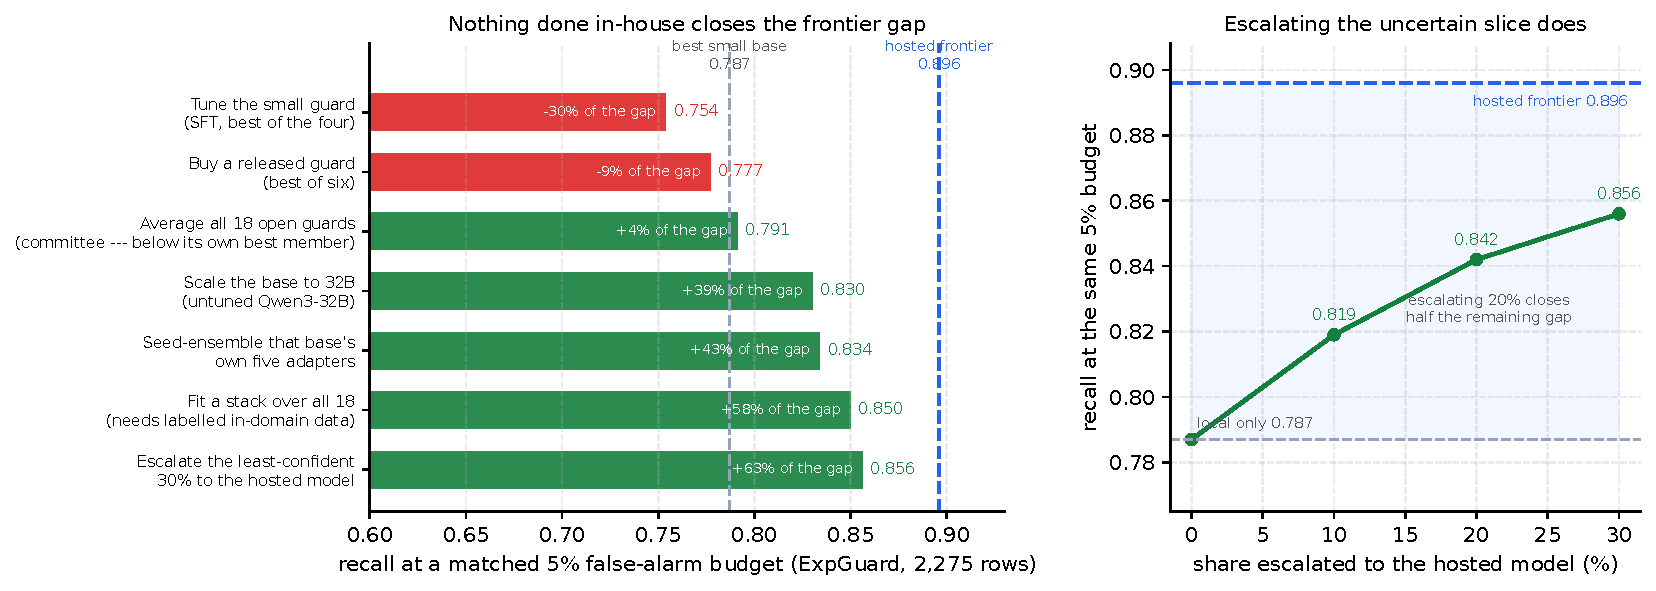
\includegraphics[width=\linewidth]{fig_gap_ladder.pdf}
\caption{\textbf{The frontier gap, and everything we tried against it} (ExpGuard, 2{,}275
expert-annotated rows; recall at a matched $5\%$ false-alarm budget so no model is read at an operating
point nobody chose). \textbf{Left:} each in-house route, with the share of the base$\to$hosted gap it
closes. Tuning the small guard and buying a released one land \emph{below} the best small base;
scale, seed-ensembling and a fitted stack move up but stall at $39$--$58\%$ of the way, and the
stack additionally needs labelled in-domain data to fit its weights. The committee bar is above the
best small base but \emph{below its own best member} --- equal weights dilute the strong members.
\textbf{Right:} the selective cascade of \Cref{sec:frontier-licenses}. Escalating the least-confident
$20\%$ of requests closes half the remaining gap; the curve is steep early because the first requests
escalated are the ones a second opinion can change. Every value is parsed from the committed generated
artifacts (\Cref{tab:frontier}, \Cref{tab:frontier-serving}, the cascade macros), so the figure cannot
drift from the tables. Retrospective, and the cascade's thresholds are selected on the rows it is then
scored on (\Cref{sec:frontier-licenses}).}
\label{fig:gap-ladder}
\end{figure}


\subsection{How large the gap is, and what buying it costs}
\label{sec:frontier-size}
\paragraph{The gain is real and it is large.} The best hosted configuration
(\FrontierBestName) reaches \FrontierBestTpr{} recall at the matched budget against
\FrontierBestBaseTpr{} for the best-performing Act~I base checkpoint \emph{on these rows}
(\FrontierBestBaseName{} --- the panel's strongest base elsewhere in this report is Qwen3-4B, and
the two swap places between instruments, which is the report's own thesis): a
paired row bootstrap on identical rows puts the difference at \FrontierGainOverBase{}
\FrontierGainOverBaseCI, an interval comfortably clear of zero. In every hundred unsafe prompts,
about eleven that the best panel base guard waves through at a $5\%$ alarm budget the frontier
model catches --- roughly half of the $21.3$ it misses. On evidence this is the largest single accuracy gap anywhere in this report, and it is
measured on the strongest label tier we have.

\paragraph{And the accuracy is bought at two orders of magnitude.} \Cref{tab:frontier-serving}
puts the price beside the gain. The best hosted configuration answers in \FrontierBestMedianMs{}\,ms
at the median against \FrontierBestBaseName's $20.1$\,ms batched forward pass (the panel spans
$10$--$25$\,ms; \Cref{tab:latency}) --- about \FrontierSlowdown$\times$ --- at roughly
\$\FrontierBestCost{} per thousand prompts against
the amortised cost of a GPU the operator already owns. For a guardrail that fires on every inbound
request, that is a budget line and a latency budget, not a rounding error. Three further costs
appear in no column of either table. Prompts leave the operator's infrastructure, which for the
mortgage setting of \Cref{sec:actIV} is a GLBA question before it is an engineering one.
The operating point is only coarsely selectable: a continuous logit margin can be placed at any
false-alarm budget exactly, while $47$--$65$ distinct integer scores can only land near one.
And the provider's own input filter refused a subset of ExpGuard prompts outright, before the
guard saw them --- \emph{non-deterministically}, with no row refused under all six configurations
and most refused under four of six. A guardrail whose input filter intermittently declines to
return a verdict, for reasons the operator cannot inspect or appeal, is a compliance artifact in
its own right.


\subsection{Routes that do not close it: tuning, scale, ensembling, purpose-built guards}
\label{sec:frontier-routes}
\paragraph{Neither tuning nor scale closes it.} Two obvious escapes suggest themselves ---
tune the small guard, or buy a bigger one --- and the same 2{,}275 rows let us price both.

\emph{Tuning does not.} Act~I's whole subject is what SFT buys, so the tuned arm belongs
here, and its effect on this external set is not a small loss but a \textbf{sign split}:
SFT changes matched-budget recall by \FrontierSftBestDelta{} on \FrontierSftBestName{} and
\FrontierSftWorstDelta{} on \FrontierSftWorstName, hurting \FrontierSftNumHurt{} of
\FrontierSftNumTotal{} checkpoints, for a panel mean of \FrontierSftMeanDelta{} that hides
swings an order of magnitude larger than itself. Within Act~I's four checkpoints the only one
SFT clearly helps is the weakest base; the three stronger ones it degrades, and on the wider
six-checkpoint set the two exceptions are that weakest base ($+0.122$) and Qwen3-8B ($+0.013$,
inside the reproduction noise floor of \Cref{sec:actI-klsft}). That is Act~I's transfer
finding --- ``a small average that hides opposite signs'' --- reproducing on \emph{external,
expert-annotated} data rather than on the inspected panel, which is a considerably stronger
test of it than Act~I could run. No tuned configuration comes near the hosted models: the
best is \FrontierBestSftName{} at \FrontierBestSftTpr.

\emph{Scale does not either.} Extending the ladder to Qwen3-8B and Qwen3-32B --- same family
as Qwen3-4B, and verified to render the frozen guard prompt to the same
\code{prompt\_template\_sha256} with the same single-token decision pair, so base size is the
only quantity varying --- makes \FrontierBestOpenName{} the strongest open guard in this study
at \FrontierBestOpenTpr. But the ladder is not clean and it does not arrive: 8B fails to
improve on 4B at all (\FrontierEightBvsFourB{} \FrontierEightBvsFourBCI, an interval that
includes zero, so we read this as ``no gain'', not as a loss), and the full
$\FrontierScaleFactor\times$ step from 4B to 32B buys \FrontierScaleGain{}
\FrontierScaleGainCI. Set that against the gap that remains to the hosted model even from
\FrontierBestOpenName: \FrontierGainOverOpen{} \FrontierGainOverOpenCI. \textbf{Everything
$\FrontierScaleFactor\times$ the parameters bought is about the size of the gap still left},
so scale alone does not close it over the range we measured --- and 32B is already far outside
the deployment envelope that motivates a small guard. We deliberately do not extrapolate a
required parameter count from this: with three points, one of them non-monotonic, no scaling
law is identified, and an earlier version of this passage claimed ``at least another order of
magnitude'' on evidence that cannot support it.

One provenance caveat governs every tuned row and is stated wherever they appear. The Act~I
\emph{release} adapters were produced on an ephemeral runner whose bucket was deleted at
cleanup and no longer exist, so the SFT rows here are the KL-SFT sweep's $\beta=0$ arm ---
same LOCK contract, same train manifest sha256, same LoRA recipe, same pinned base revisions,
but a distinct execution with different \code{adapter\_sha256} values. That is the
\code{sft\_inenv} / \code{sft\_committed} distinction \code{klsft\_summary.json} already draws
(the two agree to the third decimal on Act~I's own metrics), and these rows are labelled
\textbf{SFT (in-env)} throughout. The scale-ladder rows sit outside Act~I's locked
four-checkpoint panel by construction --- that panel is enforced in code, not merely recorded,
so extending it is impossible without invalidating the release --- and are trained and scored
through a sealed sidecar lock that copies the recipe, seeds and manifests verbatim. Act~I's
headline numbers are untouched and are not restated from either run.

\paragraph{Nor does combining what we already have.} The other instinctive response to a
vendor gap is an ensemble: we hold \FrontierEnsMembers{} open guards with ExpGuard scores ---
bases, SFT seed-ensembles, released purpose-built guards --- so combining them costs no new
training. Three combination rules, priced against the strongest single open guard
(\FrontierEnsBestSingle) and using the same rule the ensembling appendix fixes (margins average
directly within a checkpoint, rank-percentile across them). One convention note, because the same
object is quoted against two denominators in this section: the percentages \emph{in this paragraph}
are shares of the distance from that best single member to hosted, which is the question an ensemble
answers (``does combining beat picking the best?''), while \Cref{fig:gap-ladder} and the closing
summary measure every route from the best small \emph{base}, which is the question a practitioner
starts from. The stack is $\FrontierEnsStackShare\%$ of the way on the first denominator and $58\%$
on the second; both describe the same $\FrontierEnsStack$.

\emph{Seed ensembling helps, reliably and almost for free.} Averaging the five SFT seeds of a
checkpoint gains \FrontierEnsSeedGain{} matched-budget recall on average, positive for all six
checkpoints, and the adapters already exist. It is also how the tuned 32B recovers what SFT cost
it: the seed ensemble reaches \FrontierEnsBestSingle{} against $0.830$ for its own untuned base.

\emph{An unweighted committee actively hurts.} Averaging all \FrontierEnsMembers{} ranks scores
\FrontierEnsCommittee, \emph{below} the best single member --- $\FrontierEnsCommitteeShare\%$ of
the distance from that member to hosted, i.e.\ backwards. With members this unequal in quality, equal weights
dilute the strong ones; this is the \Cref{tab:frontier} spread doing exactly what one should
expect.

\emph{Even a fitted stack falls short.} A logistic stack over all \FrontierEnsMembers{} members,
scored \FrontierEnsFolds-fold out-of-fold so it cannot grade its own homework, reaches
\FrontierEnsStack{} --- $\FrontierEnsStackShare\%$ of the way from the best single member to hosted
($58\%$ of the way from the best small base). That is a real gain over
any single open guard, but it costs \FrontierEnsMembers{} forward passes per request and, less
obviously, it needs \emph{labelled in-domain data} to fit the weights, which is the asset a team
reaching for an ensemble usually does not have. Its largest weights also include a
\emph{negative} coefficient on one guard, so the fit is exploiting member-specific error
structure that may not survive a change of traffic.

So the answer is no: on ExpGuard, ensembling small guards does not beat the hosted model, and the cheap
version of it (equal weights) is worse than picking the best member. It earns its place in one
situation --- when nothing may leave the network at all, seed ensembling plus stacking is the
in-house ceiling, and it is roughly a quarter of the way to what the hosted model would give.

\paragraph{And a released guard is not the shortcut either.} The first thing a practitioner
asks is why not simply run a purpose-built guard, so \Cref{tab:frontier} carries six of them:
Qwen3Guard-Gen at 0.6B and 4B, Llama-Guard-3-1B, Granite-Guardian-3.1-2B, ShieldGemma-2B and
WildGuard-7B. Each is scored through \emph{its own} native verdict contract --- ShieldGemma's
policy-conditioned Yes/No, Granite's risk-definition Yes/No, WildGuard's
\code{Harmful request:} slot, Qwen3Guard's top-level \code{Safety:} label, Llama Guard's
\code{\textbackslash n\textbackslash nsafe}/\code{unsafe} --- because forcing our frozen prompt
on a guard would measure our prompt rather than their model. ExpGuard is also unusually fair
ground for them: none was trained on it, so unlike Act~I's dataset-held-out transfer suite ---
which includes WildGuardTest, WildGuard-7B's own benchmark --- there is no home-field advantage
to discount.

None of the six reaches the best untuned open checkpoint. The strongest,
Qwen3Guard-Gen-4B at $0.777$ and WildGuard-7B at $0.771$, sit below
\FrontierBestOpenName's \FrontierBestOpenTpr{} and well below the hosted
\FrontierBestTpr. Two land far lower --- ShieldGemma-2B at $0.458$ and Llama-Guard-3-1B at
$0.334$ --- and the reason is instructive rather than a simple lack of skill: their
\emph{ranking} is respectable (AUROC $0.865$ and $0.809$), but their negatives carry a heavy
right tail on this material. Llama Guard's 95th-percentile benign score, $+3.64$, sits
\emph{above} its median harmful score, $+2.50$, so a strict $5\%$ false-alarm budget discards
most of its recall. A guard tuned to a general web-safety taxonomy over-flags a subset of
ordinary regulated-domain questions, and that is precisely the failure a mortgage deployment
cannot absorb. It is also this report's thesis arriving from a new direction: the instrument
chooses the winner, and on regulated-domain prompts the purpose-built ordering is not the
ordering their own benchmarks report.

\label{sec:llama-guard-harness}%
One correction belongs here, because it concerns a number this repository already published.
The starting-type study's \code{llama\_guard\_3\_1b} cell is degenerate: within each of its eleven
conditions the score is a single constant on all $3{,}308$ rows --- the unmodified arm returns
$-0.125$ throughout, and each tuned seed one constant of its own --- so only three distinct values
occur in the whole $36{,}388$-row file and no adaptation can move its macro-AP
(\Cref{sec:adaptation-license}). The cause
was not the pruned output head its preflight caveat anticipated; that head is intact, and both
decision tokens carry full-norm rows. It was two independent harness bugs: under
\code{transformers}~5.x the native template rendered
\code{<BEGIN CONVERSATION>}\,\code{<END CONVERSATION>} with the user turn \emph{missing} while
still satisfying every wrapper marker, and the verdict was read at the last prompt position,
which for this contract carries the distribution over the two-newline prefix rather than over
\code{safe}/\code{unsafe}. Both are fixed (the render must now be shown to carry the payload,
and each contract's verdict prefix is teacher-forced), which is why Llama Guard scores at all
here. The published degenerate cell should be read as a harness artifact, not as a measurement
of that model.


\subsection{What scoring the ladder taught us about the specialization tax}
\label{sec:frontier-ladder}
\paragraph{A by-product worth more than the comparison that produced it.} Scoring the ladder
on Act~I's own two regimes (\Cref{tab:frontier-scale}) prices \emph{spending on parameters}
against \emph{spending on tuning}, and the two are not equivalent. SFT lifts the panel's
represented macro-AP from $0.658$ to $0.982$ and pays $-0.059$ transfer for it, with
per-checkpoint losses reaching $-0.150$. Qwen3-32B, \emph{untuned}, reaches $0.953$
represented --- within $0.029$ of the tuned panel mean --- while holding transfer at $0.962$
against the tuned panel's $0.807$. A larger base recovers most of what SFT buys
in-distribution without the transfer collapse Act~I identifies as SFT's characteristic cost.

\paragraph{And the tax tracks the distance to the endpoint.} Tuning the ladder turns this into a trend rather
than an anecdote. Ordered by how strong the base already was, SFT's represented gain
\emph{decays monotonically} while its transfer effect turns from a gain into a loss of
$0.10$--$0.15$: $+0.528/{+}0.040$ on
SmolLM2-1.7B (represented base AP $0.452$), $+0.354/-0.039$ on Qwen2.5-1.5B ($0.633$),
$+0.313/-0.087$ on SmolLM3-3B ($0.662$), $+0.098/-0.150$ on Qwen3-4B ($0.885$),
$+0.076/-0.101$ on Qwen3-8B ($0.905$), and
$\FrontierScaleTunedRepGain/\FrontierScaleTunedTransferCost$ on
\FrontierScaleTunedName{} ($0.953$). The weakest base is the only one for which SFT is
unambiguously good on both regimes; by the strongest it buys almost nothing and still charges
close to full price. One qualification the numbers force: the transfer cost is \emph{not} monotone
in base strength --- Qwen3-4B pays $-0.150$ from a $0.885$ base, more than Qwen3-8B ($-0.101$ from
$0.905$) or Qwen3-32B ($-0.117$ from $0.953$) --- so this is not a demonstrated tendency of capable
bases to specialize harder. What is regular is the \emph{endpoint}: every tuned checkpoint lands in
$0.78$--$0.85$ transfer and $0.975$--$0.990$ represented whatever its base, so the tax is the distance
to a benchmark-fixed endpoint, which is the arithmetic of \Cref{sec:actI-coupling} rather than a
behavioural law. The deployment consequence survives that reading intact: past a base of roughly
$0.9$ represented, SFT buys under $0.10$ AP and still charges close to full transfer.

\paragraph{Which answers the objection by measurement, not by extrapolation.} The obvious
challenge to the paragraph before last is that a \emph{tuned} 32B might beat an untuned one, so
we tuned it: five seeds, same recipe, same manifest. It does not.
\FrontierScaleTunedName{} goes from
$\FrontierScaleUntunedRep/\FrontierScaleUntunedTransfer$ untuned to
$\FrontierScaleTunedRep/\FrontierScaleTunedTransfer$ tuned --- buying
$\FrontierScaleTunedRepGain$ represented AP at a cost of
$\FrontierScaleTunedTransferCost$ transfer --- and on ExpGuard tuning moves its matched-budget
recall by $\FrontierScaleTunedExpguardDelta$, the wrong way. For a guardrail, whose entire
purpose is the traffic nobody anticipated, that is a bad trade at any size. Across the six
checkpoints we can now tune, SFT hurts \FrontierSftNumHurt{} of \FrontierSftNumTotal{} on
external held-out prompts, and on ExpGuard the best tuned configuration in this study
(\FrontierBestSftName{} at \FrontierBestSftTpr) still sits well below the hosted model's
\FrontierBestTpr. That ordering is specific to this external, never-trained-on probe:
\Cref{sec:actIII-h2h} shows it reverses on sources the panel does represent.

One limit keeps the untuned-32B result from being a recommendation: it is a deployment-choice
contrast, not a controlled one. Qwen3-32B is $8$--$21\times$ the parameters of the panel
checkpoints and costs accordingly, so the comparison is about \emph{where} to spend a fixed
budget, not about SFT being inferior at equal size. What the tuned-32B cell does establish is
narrower and still useful: at \emph{that} size, on \emph{this} recipe and data, tuning is not
the way to spend the next increment.


% GENERATED by reproduce.py from artifacts/expguard_external/ (frontier.py)
\begin{table}[H]\centering\footnotesize
\caption{Frontier hosted guardrails against this report's local guards on ExpGuard (2,275 expert-annotated finance/health/law prompts), joined by row hash so every guard is scored on identical rows. \textbf{TPR@5\%FPR} is recall at a matched false-alarm budget --- each guard is re-thresholded on these rows to a common $5\%$ FPR, because the models sit at very different self-chosen operating points (the frontier configs alarm on only $2.3$--$3.4\%$ of negatives at their own verdict). Local guards rank by the raw margin $z_{\text{unsafe}}-z_{\text{safe}}$; frontier guards by a self-reported integer risk, the only graded signal the Responses API exposes for reasoning models. SFT rows are the \emph{in-env} beta$=0$ re-execution of the Act~I recipe, not the Act~I release adapters (different \code{adapter\_sha256}); Act~I's numbers are unchanged and not restated here.}
\label{tab:frontier}
\begin{tabular}{lrrrrrrr}\toprule
Guard & $n$ & TPR@5\%FPR & AP & AUROC & AP fin & AP health & AP law \\
\midrule
\multicolumn{8}{l}{\emph{Act~I panel, base (zero-shot)}} \\
Qwen2.5-1.5B (1.5B) & 2275 & .668 & .9208 & .8955 & .9383 & .9056 & .9177 \\
SmolLM2-1.7B (1.7B) & 2275 & .510 & .8832 & .8399 & .8869 & .8921 & .8679 \\
SmolLM3-3B (3B) & 2275 & .787 & .9561 & .9351 & .9579 & .9545 & .9579 \\
Qwen3-4B (4B) & 2275 & .768 & .9506 & .9273 & .9570 & .9377 & .9568 \\
\midrule
\multicolumn{8}{l}{\emph{Act~I panel, SFT (in-env), mean of 5 seeds}} \\
Qwen2.5-1.5B (1.5B) & 2275 & .658 & .9103 & .8874 & .9304 & .8885 & .9241 \\
SmolLM2-1.7B (1.7B) & 2275 & .632 & .9121 & .8764 & .9152 & .9092 & .9154 \\
SmolLM3-3B (3B) & 2275 & .727 & .9353 & .9149 & .9526 & .9065 & .9541 \\
Qwen3-4B (4B) & 2275 & .754 & .9349 & .9087 & .9431 & .9174 & .9513 \\
\midrule
\multicolumn{8}{l}{\emph{Scale-ladder extension, base (zero-shot; outside the locked panel)}} \\
Qwen3-8B (8B) & 2275 & .748 & .9436 & .9239 & .9426 & .9432 & .9532 \\
Qwen3-32B (32B) & 2275 & .830 & .9633 & .9445 & .9685 & .9538 & .9699 \\
\midrule
\multicolumn{8}{l}{\emph{Scale-ladder extension, SFT (in-env), mean of 5 seeds}} \\
Qwen3-8B (8B) & 2275 & .761 & .9355 & .9102 & .9448 & .9126 & .9552 \\
Qwen3-32B (32B) & 2275 & .809 & .9563 & .9402 & .9646 & .9389 & .9714 \\
\midrule
\multicolumn{8}{l}{\emph{Frontier, hosted API (zero-shot)}} \\
\textbf{gpt-5.4 (low)} & 2275 & .896 & .9773 & .9691 & .9795 & .9736 & .9812 \\
\textbf{gpt-5.4 (medium)} & 2264 & .892 & .9770 & .9691 & .9799 & .9685 & .9852 \\
\textbf{gpt-5.4 (high)} & 2259 & .894 & .9779 & .9709 & .9819 & .9704 & .9818 \\
\textbf{gpt-5.4-mini (low)} & 2255 & .885 & .9726 & .9623 & .9766 & .9609 & .9806 \\
\textbf{gpt-5.4-mini (medium)} & 2256 & .886 & .9729 & .9634 & .9771 & .9658 & .9750 \\
\textbf{gpt-5.4-mini (high)} & 2254 & .883 & .9740 & .9665 & .9796 & .9602 & .9795 \\
\bottomrule
\end{tabular}\\[3pt]{\footnotesize \textbf{Paired comparison} (gpt-5.4 (low) $-$ Qwen3-32B base, the strongest open guard here, on the 2,275 rows both scored; 2,000-resample paired row bootstrap). $\Delta$TPR@5\%FPR $= +0.0661$ $[+0.0428, +0.0893]$; $\Delta$AP $= +0.0140$ $[+0.0098, +0.0188]$. Within the Qwen3 family, $8\times$ the parameters (4B~$\to$~32B) buys $\Delta$TPR $= +0.0621$ $[+0.0395, +0.0842]$ --- about as much as the gap that remains. Against the strongest tuned guard (Qwen3-32B SFT in-env), averaged over its 5 seeds: $\Delta$TPR@5\%FPR $= +0.0865$, $\Delta$AP $= +0.0210$. The frontier score is a coarse integer 0--100 risk with heavy ties, which caps AP resolution, so these deltas are conservative.}
\end{table}
                % tab:frontier (base vs SFT in-env vs frontier)
% GENERATED by reproduce.py from artifacts/ (frontier.py)
\begin{table}[H]\centering\small
\caption{Scaling the base versus tuning a small one, on Act~I's own two regimes (macro-AP; represented $=$ in-distribution sources on \code{id\_test}, transfer $=$ held-out sources on \code{transfer\_test}). The convention here reproduces Act~I's committed \code{base\_represented} and \code{base\_transfer} to four decimals for all four panel checkpoints, which is what licenses placing extension rows beside them. SFT buys represented AP and pays for it in transfer; a larger \emph{untuned} base buys much of the same represented AP and keeps its transfer. These are inspected-panel numbers and are reported apart from --- never pooled with --- the external ExpGuard numbers in \Cref{tab:frontier}. The scale rows are a deployment-choice contrast, not a controlled one: Qwen3-32B is $8$--$21\times$ the parameters of the panel checkpoints and costs accordingly.}
\label{tab:frontier-scale}
\begin{tabular}{lrrr}\toprule
Guard & Params (B) & Represented AP & Transfer AP \\
\midrule
\multicolumn{4}{l}{\emph{Act~I panel, base (zero-shot)}} \\
Qwen2.5-1.5B & 1.5 & .6334 & .8187 \\
SmolLM2-1.7B & 1.7 & .4524 & .7904 \\
SmolLM3-3B & 3 & .6621 & .9102 \\
Qwen3-4B & 4 & .8855 & .9438 \\
\midrule
\multicolumn{4}{l}{\emph{Act~I panel after SFT, mean of 4 checkpoints (committed release adapters)}} \\
Panel mean, SFT & -- & .9818 & .8069 \\
\midrule
\multicolumn{4}{l}{\emph{Scale ladder, base (zero-shot; outside the locked panel)}} \\
\textbf{Qwen3-8B} & 8 & .9052 & .9410 \\
\textbf{Qwen3-32B} & 32 & .9533 & .9620 \\
\midrule
\multicolumn{4}{l}{\emph{Scale ladder after SFT (in-env), mean of 5 seeds}} \\
Qwen3-8B, SFT & 8 & .9814 & .8398 \;\footnotesize$(+0.076,\,-0.101)$ \\
\bottomrule
\end{tabular}
\end{table}
          % tab:frontier-scale (scale vs tuning, Act I regimes)
% GENERATED by reproduce.py from artifacts/expguard_external/ (frontier.py)
\begin{table}[H]\centering\small
\caption{What the frontier accuracy in \Cref{tab:frontier} costs to serve. Local P50 is the committed batched A100 figure from \Cref{tab:latency}; frontier latency is measured on the ExpGuard rows themselves at concurrency 200 (throughput-regime, an upper bound on an isolated request). Dollar figures are billed tokens at assumed public list prices --- an estimate, not billing truth --- and exclude the fixed cost of owning a GPU, which is what the self-hosted column elides. The trade is roughly two orders of magnitude in median latency against about \emph{halving} the misses: at a matched $5\%$ budget the hosted model misses $10.4\%$ of unsafe prompts against the best small base's $21.3\%$ ($2.0\times$ fewer) and the best $32$B open base's $17.0\%$ ($1.6\times$ fewer). An earlier version of this caption said \emph{one order of magnitude} fewer misses, which was simply wrong. Three properties also do not appear in any column: prompts leave the operator's infrastructure, the operating point is only coarsely selectable, and the provider may refuse a prompt before the guard ever sees it.}
\label{tab:frontier-serving}
\begin{tabular}{lrrrr}\toprule
Guard & P50 (ms) & P99 (ms) & \$/1k prompts & TPR@5\%FPR \\
\midrule
\multicolumn{5}{l}{\emph{Local guards --- one forward pass, batched on A100}} \\
Qwen2.5-1.5B (SFT) & 10.4 & -- & self-hosted & .658 \\
SmolLM2-1.7B (SFT) & 11.9 & -- & self-hosted & .632 \\
SmolLM3-3B (SFT) & 20.1 & -- & self-hosted & .727 \\
Qwen3-4B (SFT) & 25.2 & -- & self-hosted & .754 \\
\midrule
\multicolumn{5}{l}{\emph{Frontier --- hosted API, measured on the ExpGuard rows}} \\
\textbf{gpt-5.4 (low)} & 1,553 & 4,523 & \$0.80 & .896 \\
\textbf{gpt-5.4 (medium)} & 1,837 & 6,424 & \$1.18 & .892 \\
\textbf{gpt-5.4 (high)} & 2,009 & 6,594 & \$1.60 & .894 \\
\textbf{gpt-5.4-mini (low)} & 1,665 & 16,933 & \$0.18 & .885 \\
\textbf{gpt-5.4-mini (medium)} & 1,638 & 7,161 & \$0.29 & .886 \\
\textbf{gpt-5.4-mini (high)} & 1,804 & 5,909 & \$0.41 & .883 \\
\bottomrule
\end{tabular}
\end{table}
        % tab:frontier-serving (latency + $/1k)

\subsection{The frontier gap is a property of the regime, not of the model}
\label{sec:actIII-h2h}
Everything above measures the gap on ExpGuard, and that choice does more work than it looks
like. ExpGuard is an \emph{external breadth probe}: no guard in this report was trained on it,
which is exactly what makes it a clean instrument --- and also means it reports the
\emph{transfer} regime and nothing else. The $\FrontierGainOverBase$ figure is therefore the
transfer gap, not the gap.

Five of the general-safety corpora the GPT baseline scored are also scored by the Act~I panel,
and those rows can be joined: the two runs simply hash their row identities differently
(\code{sha256(text)[:16]} against \code{content\_sha256}, which normalizes first), so
re-deriving both digests from the local corpus recovers the mapping for $100\%$ of the panel's
rows. The regime split is then read from Act~I's own manifest rather than asserted ---
\code{train.jsonl} is exactly \HtwoRepSources{} --- so \code{id\_test} rows are held-out
\emph{rows} from a \emph{represented} source, while \code{transfer\_test} sources are held out
at the source level.

\Cref{tab:h2h} is the result, at the same matched \HtwoBudget{} budget. It reverses direction
across the split. On represented sources the panel's small tuned guards \emph{beat} the frontier
reference. The summary we report is an \emph{aggregate} that does not depend on which cell wins:
the equal-source, equal-checkpoint mean paired difference over the \HtwoNRepSources{} represented
sources is \HtwoAggDeltaTpr{} \HtwoAggDeltaTprCI{} in recall at the matched budget, and
\HtwoAggDeltaAp{} \HtwoAggDeltaApCI{} in AP; both exclude zero. \Cref{fig:regime-map} is that
reversal in one picture.

\begin{figure}[htbp]\centering
% A matrix, not hand-placed nodes: an earlier hand-placed version let the row labels run under
% the cells, because a node's `text width` and its centre have to be reconciled by hand.
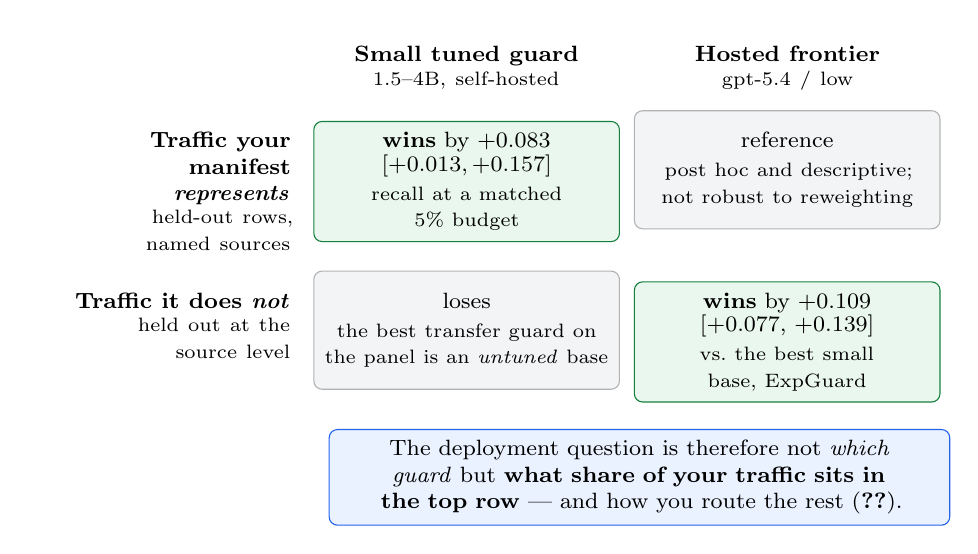
\begin{tikzpicture}[font=\footnotesize,
  cellbase/.style={rounded corners=3pt,align=center,inner sep=4pt,text width=3.6cm,
                   minimum height=1.5cm},
  win/.style={cellbase,draw=tkgreenedge,fill=tkgreen},
  lose/.style={cellbase,draw=black!30,fill=cardgrey},
  hdr/.style={align=center,font=\footnotesize\bfseries,text width=3.6cm},
  rlab/.style={align=right,font=\footnotesize\bfseries,text width=3.1cm}]
\matrix (m) [matrix of nodes, nodes in empty cells, row sep=4pt, column sep=5pt,
             ampersand replacement=\&] {
  \& |[hdr]| {Small tuned guard\\[-1pt]\normalfont\scriptsize 1.5--4B, self-hosted}
  \& |[hdr]| {Hosted frontier\\[-1pt]\normalfont\scriptsize \HtwoRef} \\
  |[rlab]| {Traffic your manifest\\\emph{represents}\\[-1pt]\normalfont\scriptsize held-out rows,
            named sources}
  \& |[win]| {\textbf{wins} by \HtwoAggDeltaTpr\\[-1pt]\HtwoAggDeltaTprCI\\[1pt]
              \scriptsize recall at a matched \HtwoBudget{} budget}
  \& |[lose]| {reference\\[1pt]\scriptsize post hoc and descriptive; not robust to reweighting} \\
  |[rlab]| {Traffic it does \emph{not}\\[-1pt]\normalfont\scriptsize held out at the
            source level}
  \& |[lose]| {loses\\[1pt]\scriptsize the best transfer guard on the panel is an \emph{untuned}
               base}
  \& |[win]| {\textbf{wins} by \FrontierGainOverBase\\[-1pt]\FrontierGainOverBaseCI\\[1pt]
              \scriptsize vs.\ the best small base, ExpGuard} \\
};
\node[draw=bgblueedge,fill=bgblue,rounded corners=3pt,inner sep=4pt,align=center,
      text width=7.6cm,below=6pt of m.south east,anchor=north east]
     {The deployment question is therefore not \emph{which guard} but \textbf{what share of your
      traffic sits in the top row} --- and how you route the rest (\Cref{sec:frontier-licenses}).};
\end{tikzpicture}
\caption{\textbf{The frontier gap is a property of the regime, not of the model.} The same
comparison, at the same matched \HtwoBudget{} false-alarm budget, points in opposite directions on
the two regimes: a hosted frontier model is the better ranker on prompts from sources nobody trained
on, and the panel's small \emph{tuned} guards are the better rankers on sources the training manifest
names. The top-left cell is a post-hoc descriptive summary over \HtwoNRepSources{} purposively chosen
corpora and is \emph{not} robust to reweighting (\Cref{tab:h2h-weighting}); the bottom-right is a
paired comparison on external expert-annotated rows. The two cells sit at the same evidence flavor
(retrospective) but on different data, and are never pooled.}
\label{fig:regime-map}
\end{figure}

\textbf{This aggregate is post hoc and is reported as a descriptive fixed-panel summary, not as a
test.} It did not exist before the per-cell headline failed multiplicity --- it was added in the
same revision that found the failure. It is a sounder summary than the maximum of twelve, because
its weighting is fixed by the regime split rather than by any result, but that is not the same as
having been specified in advance, and we do not claim it was. Only a summary frozen before a fresh
cohort is scored could carry a confirmatory frontier claim.

\paragraph{Two things the interval is conditional on, stated before the sensitivities.} It is
conditional on \emph{these three sources}. The bootstrap holds the source set fixed and resamples
evaluation families within it, because three purposively chosen corpora do not sample a population
of corpora. Drawing sources with replacement instead --- the unconditional version --- widens the
interval to \HtwoAggSrcResampledCI, which \emph{includes} zero. That is the honest statement of how
far the result travels: it is a claim about the panel's behaviour on \code{toxicchat},
\code{prompt\_injections} and \code{jailbreak\_classification}, not about represented sources in
general. It is also conditional on the seed pairing: seeds $42$--$46$ are the same five training
runs on every source, so the joint bootstrap draws one seed vector per checkpoint and reuses it
across sources rather than redrawing independently, which would break the pairing that carries
most of the covariance.

\paragraph{The headline is not robust to how the same twelve cells are weighted.} The weighting
choice matters enough that giving only the one we report would be misleading, so
\Cref{tab:h2h-weighting} gives all four --- each from the same joint bootstrap draws, so they are
mutually comparable rather than four separate analyses. \textbf{Only two of the four support a
positive advantage at all}: weighting sources by their row counts roughly halves the estimate and
straddles zero (the largest source, \code{toxicchat} at $n=451$, carries the smallest effect,
$+0.028$ against $+0.157$ on \code{prompt\_injections}), and including the \emph{base} arms
alongside the tuned ones excludes zero in the \emph{opposite} direction.

That last row is the one to keep in view, because it says what the result is about: the
represented-source advantage is a property of \emph{tuned} guards specifically --- Act~I's
specialization seen from the other side --- and not a general statement that small guards beat
hosted ones. On transfer sources the ordering flips back, the reference leads (\HtwoTransRefTpr{} on
\code{xstest} against \HtwoTransBestLocalName{}'s \HtwoTransBestLocalTpr), and tuning is what costs
the guard its position: the strongest transfer guard in the panel is an \emph{untuned} base.

\begin{table}[htbp]\centering\small
\caption{\textbf{The same twelve cells, four defensible weightings.} $\Delta$TPR at the matched
\HtwoBudget{} budget, panel SFT minus \HtwoRef, over the \HtwoNRepSources{} represented sources; all
four from the \emph{same} joint bootstrap draws (evaluation families and training seeds resampled,
source set held fixed). The first row is the one reported in the abstract and in
\Cref{tab:glance}; it is post hoc, and the table is here so a reader can see how much of the
conclusion rests on the choice.}
\label{tab:h2h-weighting}
\setlength{\tabcolsep}{6pt}\renewcommand{\arraystretch}{1.15}
\begin{tabular}{@{}lrlc@{}}
\toprule
Weighting of the \HtwoNCells{} cells & $\Delta$TPR & $95\%$ interval & Excludes zero? \\
\midrule
Equal per source \textit{(reported)} & \HtwoAggEqSourceTpr & \HtwoAggEqSourceTprCI & \cmark \\
Equal per cell & \HtwoAggEqCellTpr & \HtwoAggEqCellTprCI & \cmark \\
Proportional to rows per source & \HtwoAggRowWTpr & \HtwoAggRowWTprCI & \xmark \\
Equal per cell, \emph{including the base arms} & \HtwoAggWithBaseTpr & \HtwoAggWithBaseTprCI &
\cmark\ \emph{(opposite sign)} \\
\midrule
\multicolumn{4}{@{}l}{\itshape Sensitivity to the source set, not the weighting:} \\
Equal per source, sources \emph{resampled} & \HtwoAggEqSourceTpr & \HtwoAggSrcResampledCI & \xmark \\
\bottomrule
\end{tabular}
\end{table}

\paragraph{The largest single cell is exploratory, and does not survive multiplicity.} The most
striking cell is \HtwoBestName{} --- a \emph{1.5B} model --- at \HtwoBestTpr{} on
\HtwoBestSource{} against the reference's \HtwoRefTpr, i.e.\ \HtwoBestDeltaTpr{} with a
nominal interval of \HtwoBestDeltaTprCI{} and a ranking rather than a threshold advantage
(AUROC \HtwoBestAuroc{} against \HtwoRefAuroc). That cell is \emph{selected as the maximum of
\HtwoNCells{}}, so its nominal interval is post-selection and overstates the evidence. Two
familywise objects, because they answer different questions. As a \emph{decision}: a Holm
step-down over the \HtwoNCells{} represented-source SFT cells, on two-sided percentile-bootstrap
$p$-values, rejects nothing --- this cell's $p=\HtwoBestPBoot$ against a first threshold of
$\alpha/12=\HtwoHolmFirstThreshold$ (adjusted $p=\HtwoBestPHolm$), so \HtwoNSigNominal{} of
\HtwoNCells{} cells clear zero nominally and \HtwoNSigHolm{} survive the correction. As an
\emph{interval}: Holm controls decisions and does not produce intervals, so the band we quote is
max-$T$ over the same twelve cells, standardised by each cell's own bootstrap spread with the
critical value $c=\HtwoMaxTCrit$ read off the joint draws, giving \HtwoBestDeltaTprHolm{}, which
includes zero. An earlier revision printed a narrower band here and called it Holm-adjusted; it
was neither --- it rescaled percentile bounds by a ratio of \emph{normal} critical values and
ranked the cells by $|\Delta|$ over half-width rather than by $p$, with no step-down stopping.
The qualitative answer is unchanged, and it could only ever have moved one way: the omitted
stopping rule made the old procedure anti-conservative, so ``none survive'' was already the
generous reading. The per-cell numbers are
therefore reported as exploratory throughout, and no sentence in this report should be read as
``a 1.5B guard beats the frontier'' on the strength of one cell. What the aggregate supports is
weaker and still substantive: \emph{on average across represented sources}, the panel's tuned
guards rank unsafe prompts better than the hosted reference at a matched alarm budget.

An earlier version of this subsection reported \HtwoBestDeltaTpr{} as $+0.185$ with a narrower
interval. That number came from a different estimand than the one tabulated beside it --- the
metric of a five-seed \emph{score ensemble} rather than the mean of five per-seed metrics --- so
the difference did not equal the two values it sat between, and it carried no training-seed
uncertainty. The estimator is now the mean of per-seed paired differences with evaluation families
and seeds both resampled, which makes every delta equal the arithmetic difference of the two
tabulated values by construction and widens the intervals accordingly. A later revision made one
further change to the same intervals: the bootstrap resamples \code{family\_id} clusters rather
than bare rows, so this table now uses the same family-aware uncertainty protocol as the rest of
the report instead of a second, looser one. That widened the per-cell intervals slightly and moved
the count of nominally significant cells from four to \HtwoNSigNominal{}.

% GENERATED by experiments/emit_frontier_general_h2h_tex.py from artifacts/frontier_general_h2h/h2h.json
\begin{table}[H]\centering\footnotesize
\caption{\textbf{The frontier gap is a property of the regime, not of the model size.} TPR at a matched \HtwoBudget{} false-alarm budget on the five general-safety corpora that both the Act~I panel and the GPT baseline scored, joined by re-deriving each side's row digest from the local corpus (100\% of the panel's rows join; \code{join\_audit.json}). The regime split is read from Act~I's own manifest, not asserted: \emph{represented} sources appear in \code{train.jsonl} (these are held-out \emph{rows} from them, \code{id\_test}); \emph{transfer} sources are held out at the source level (\code{transfer\_test}). On represented sources the small tuned guards beat the frontier reference; on transfer sources they lose to it, and tuning is what costs them. This is why \Cref{tab:frontier}, which measures ExpGuard alone --- an external source the panel never trained on --- sees only the second half of that picture. Retrospective and estimation-only: these rows and this panel were inspected during development. \textdagger{} marks a TPR whose threshold fell inside a tie block of a coarse score, so the cell is an artifact of the ties and not a behaviour --- read its AUROC in \code{h2h.json} instead.}
\label{tab:h2h}
\begin{tabular}{lrrrrr}\toprule
& \multicolumn{3}{c}{\emph{represented}} & \multicolumn{2}{c}{\emph{transfer}} \\
\cmidrule(lr){2-4}\cmidrule(lr){5-6}
Guard & \textbf{jb\_class.} & \textbf{prompt\_inj.} & \textbf{toxicchat} & jbbench & xstest \\
\midrule
\multicolumn{6}{l}{\emph{Act~I panel, base (zero-shot)}} \\
Qwen2.5-1.5B & .000 & .074 & .319 & \textdagger{}.200 & \textdagger{}.167 \\
SmolLM2-1.7B & .000 & .000 & .184 & .600 & .575 \\
SmolLM3-3B & .025 & .074 & .444 & .767 & .867 \\
Qwen3-4B & .557 & \textdagger{}.296 & .681 & .867 & .917 \\
\midrule
\multicolumn{6}{l}{\emph{Act~I panel, SFT (mean of 5 seeds)}} \\
Qwen2.5-1.5B & .985 & .948 & .882 & .217 & .487 \\
SmolLM2-1.7B & .985 & .911 & .816 & .367 & .700 \\
SmolLM3-3B & .990 & .852 & .868 & .437 & .588 \\
Qwen3-4B & .995 & .881 & .889 & .257 & .590 \\
\midrule
\multicolumn{6}{l}{\emph{Frontier, hosted API (zero-shot)}} \\
\textbf{gpt-5.4 (low)} & .924 & .741 & .836 & \textdagger{}.100 & .967 \\
gpt-5.4 (medium) & .924 & .704 & .874 & .750 & .967 \\
gpt-5.4 (high) & .937 & .667 & .894 & .767 & .975 \\
gpt-5.4-mini (low) & .962 & .556 & .845 & .850 & .942 \\
gpt-5.4-mini (medium) & .962 & .519 & .845 & .767 & .917 \\
gpt-5.4-mini (high) & .937 & .593 & .860 & .883 & .942 \\
\bottomrule
\end{tabular}\\[3pt]{\footnotesize \textbf{Paired comparison} against \HtwoRef{} on the rows both scored (\HtwoNBoot{}-resample paired row bootstrap, 95\% CI). Strongest represented-source result: \HtwoBestName{} SFT on \HtwoBestSource{} ($n=\HtwoBestN$), $\Delta$TPR@\HtwoBudget{}FPR $=$ \HtwoBestDeltaTpr{} \HtwoBestDeltaTprCI{}, $\Delta$AP $=$ \HtwoBestDeltaAp{} \HtwoBestDeltaApCI{} --- a \emph{ranking} win (AUROC \HtwoBestAuroc{} vs.\ \HtwoRefAuroc{}), not a threshold placement. \HtwoNSig{} of \HtwoNSftCells{} panel-SFT cells on represented sources clear zero at the 95\% level. The \code{jailbreakbench} column carries no deltas: the reference's own TPR there is tie-collapsed (\textdagger), so differences against it are uninterpretable. Per-source $n$ is small (67--451 rows), so these intervals are wide and no per-cell ordering should be read as a ranking.}
\end{table}
                   % tab:h2h (represented vs transfer, both regimes)

Four limits bound this, and they matter more than the headline. Per-source $n$ is $67$--$451$,
so the intervals are wide and no per-cell ordering is a ranking. The evidence is
\textbf{retrospective and estimation-only} --- these rows and this panel were inspected during
development --- so it sits at the same flavor as Acts~I--II in \Cref{tab:ledger} and is never
pooled with the ExpGuard numbers above despite appearing beside them. A represented-source win
is not a claim about novel traffic: it says a guard beats the frontier on distributions an
operator can enumerate in training, which is a deployment property and not a capability claim.
And \code{id\_test} is held out by \emph{row}, not by content --- the overlap audit
(\Cref{sec:not-establish}) puts $1.6\%$--$5.0\%$ of each represented split within
Jaccard~$0.70$ of a training row, which qualifies these margins rather than overturning them,
most of all on \code{jailbreak\_classification}.

What survives all four is a statement about \emph{where} the frontier earns its price. It is not
buying a uniformly better guard; it is buying the regime a small guard is worst at. That
reframes the practical question from ``can a small guard match the frontier'' to ``how much of
your traffic resembles something you can put in a training manifest'' --- and it is the
motivation for a routing rule keyed to \emph{unfamiliarity} rather than to score margin. That
rule is a \textbf{hypothesis this report does not test}: the only cascade measured here
(\Cref{sec:frontier-licenses}) escalates by rank distance to the local guard's own decision line,
which is itself a margin router, and no familiarity detector is implemented or evaluated anywhere
in this work.

\subsection{Which requests, and what this licenses}
\label{sec:frontier-licenses}
\paragraph{The deployment question is not which guard, but which requests.} Everything above
compares whole guards, which frames the choice as self-host \emph{or} outsource. That framing
is wrong, and the per-row scores show why. Run the small guard inline on every request, rank
requests by how near they fall to its own decision line, and re-score only that uncertain band
with the hosted model, holding one global $5\%$ false-alarm budget across the whole
construction. Escalating the least-confident $10\%$ of ExpGuard raises matched-budget recall
from \CascadeLocalOnly{} to \CascadeTen{}; $20\%$ reaches \CascadeTwenty{}, which is
\emph{half} the distance to the hosted model's \FrontierBestTpr; $30\%$ reaches
\CascadeThirty{}. The curve is steep early because the
first requests escalated are the ones a second opinion can actually change, and it is smooth,
so the escalated share is a dial set by whatever the data-residency and cost constraints
allow rather than an architecture to be chosen once. Two implementation notes, since the
construction is easy to get wrong: the two guards are fused on \emph{rank}, because a logit
margin and a self-reported integer risk are not on a common scale; and a per-band threshold
was tried first and rejected, because with a small escalated slice there are too few deferred
negatives to place a stable quantile, which made the curve non-monotone for purely numerical
reasons. This is a retrospective analysis on committed scores, not a deployed system: it
assumes the escalated subset may lawfully leave, which for the mortgage traffic of
\Cref{sec:actIV} is exactly the question that has to be answered first.

\paragraph{What this does and does not license.} It licenses one sentence: on external,
expert-annotated finance/health/law prompts, a hosted frontier model is a materially more
accurate prompt-safety ranker than any small guard in this report, tuned or not, and the margin
survives a paired test. It does \emph{not} license extending that to the mortgage construct of
\Cref{sec:actIV}: ExpGuard is single-label general prompt safety, not the dual
$G\times D$ compliance judgement, and nothing here was measured on it. Nor does it retire the
report's subject. Acts~I--II are about what happens \emph{when} you must run a small guard
yourself --- for latency, cost, data residency, or auditability --- and this subsection prices
that constraint rather than dissolving it. The honest reading is that the frontier number is the
bar \emph{on unfamiliar traffic}: it is what the specialization and composition machinery is
trying to reach under constraints the hosted model does not have to satisfy. On traffic the
operator can enumerate, \Cref{sec:actIII-h2h} shows the bar is already cleared --- which is
why the deployment question is a routing question rather than a modelling one.

\edb{On external expert-annotated rows at a matched \HtwoBudget{} alarm budget, the best hosted
configuration (\FrontierBestName) beats the strongest panel base by \FrontierGainOverBase{}
\FrontierGainOverBaseCI{} recall, and nothing in-house closes it: tuning and released guards land
\emph{below} the best small base, and scale, seed-ensembling and a fitted stack reach only
$39$--$58\%$ of the way (\Cref{fig:gap-ladder}). Escalating the least-confident $30\%$ reaches
\CascadeThirty{}. On \emph{represented} sources the ordering reverses (\Cref{fig:regime-map}).}
{Self-host the traffic you can enumerate in a training manifest, and escalate the slice your own
guard is least sure about --- the escalated share is a dial, not an architecture. Price the hosted
path at $\approx\FrontierSlowdown\times$ the median latency and \$\FrontierBestCost/1k prompts, and
answer the data-residency question before the accuracy one.}
{Retrospective and estimation-only. The cascade's decision line and its global \HtwoBudget{} threshold
are both selected on the rows it is then scored on, so the curve is optimistically tuned; the router
tested is a \emph{margin} router, and the unfamiliarity router this section makes attractive is
untested. The represented-source reversal is a post-hoc summary over three purposively chosen corpora
and is not robust to reweighting (\Cref{tab:h2h-weighting}). Nothing here extends to the dual
$G\times D$ mortgage construct.}


\section{Synthesis: what benchmark gains do --- and do not --- predict}
\label{sec:synthesis}
The four questions have one answer. A guard's benchmark score is co-produced by the benchmark: SFT buys
represented-source ranking, not transfer --- and at an equal false-alarm budget it does not even buy the
recall it appears to, catching \MatchedTransferSft{} against its own base's \MatchedTransferBase{}
off-source (Act~I); keeping the base in an output-space average
\emph{recovers} some transfer without retraining (at a second inference pass), though not a threshold (Act~II); and a change of
domain can hide the violation entirely, so regulated domains need domain-grounded evaluation and a
fairness gate (Act~III) --- and building that gate taught us that the gate itself needs the same
scrutiny as the guards: ours does not survive it (\Cref{sec:actIV-mortgage-pairs}).
The recurring cast makes it concrete: Qwen3-4B, the strongest base, specializes the most on transfer,
is the one composition hurts, yet is \emph{numerically} the best-ranking zero-shot mortgage
guard (on a small split, so read as a direction) --- the ranking flips with the benchmark.

The frontier comparison (\Cref{sec:actIII-frontier}) then turns the same lesson outward, and this is
where the caution acquires a deployment-facing shape: the choice stops being \emph{which guard}
and starts being \emph{which traffic}. A hosted model is the more accurate ranker on
\emph{unfamiliar} prompts, but on sources an operator can enumerate in a training manifest the ordering
inverts: averaged over the represented sources the panel's tuned guards rank better than the
reference by \HtwoAggDeltaTpr{} \HtwoAggDeltaTprCI{} at the matched budget (\Cref{sec:actIII-h2h};
individual cells are exploratory and none survives a familywise correction). So the gap is not a capability ceiling to be closed by a larger student --- it is
the price of the regime, and the practical question is not \emph{which guard} but \emph{what share of
your traffic you can characterise in advance}. That suggests routing on \emph{unfamiliarity} rather than on
score margin --- but it is a suggestion, not a result. The cascade we actually measured
(\Cref{sec:frontier-licenses}) is a margin router, so this report contains evidence about margin
routing and none about familiarity routing; the regime result motivates that comparison rather
than settling it.

\Cref{tab:guidelines} distills the whole study into the guideline each finding implies: what we
learned, the evidence for it here, and what a practitioner should therefore \emph{do}. Every row is
anchored to a result in this report; where a finding is directional (small split) or fixed-panel, the
guideline is qualified accordingly.

\begingroup\small
\renewcommand{\arraystretch}{1.4}
\setlength{\extrarowheight}{2.5pt}
\arrayrulecolor{guiderule}
\begin{longtable}{@{}>{\raggedright\arraybackslash}p{0.235\linewidth} >{\raggedright\arraybackslash}p{0.335\linewidth} >{\raggedright\arraybackslash}p{0.35\linewidth}@{}}
\caption{What this study establishes, and the professional guideline each finding implies. Numbers are
macro-AP deltas from the fixed panel (represented $=$ in-distribution sources, transfer $=$ held-out
sources); CIs/LCBs are one-sided bootstrap bounds. Acts~I--II are retrospective estimation on an
inspected panel (\emph{not} preregistered/confirmatory --- see limitations); only the adaptation
study is preregistered. Read directional rows (marked) as a direction, not a verdict.}
\label{tab:guidelines}\\
% The heading row must sit INSIDE the \endfirsthead / \endhead blocks. It previously sat after
% \endhead, i.e. as the first body row, so it printed once and the continuation page carried a
% bare rule with no column titles.
\rowcolor{tkgreenedge}
{\color{white}\bfseries What we learned} & {\color{white}\bfseries Evidence (this study)} & {\color{white}\bfseries Guideline: what to do} \\
\endfirsthead
\multicolumn{3}{@{}l}{\small\itshape \Cref{tab:guidelines}, continued}\\
\rowcolor{tkgreenedge}
{\color{white}\bfseries What we learned} & {\color{white}\bfseries Evidence (this study)} & {\color{white}\bfseries Guideline: what to do} \\
\endhead

\rowcolor{white}
\textbf{\textcolor{tkgreenedge}{1.}~A guard's ranking is co-produced by the benchmark --- it flips across benchmarks.} &
Qwen3-4B is the worst transfer specializer yet the numerically best-ranking zero-shot mortgage guard
(\Cref{tab:baseline}, \Cref{tab:expguard}; directional/small split). &
Never rank guards on a single leaderboard; score \emph{your} candidates on represented, held-out,
over-refusal, and domain sets. \\
\rowcolor{guidealt}
\textbf{\textcolor{tkgreenedge}{2.}~Ordinary SFT buys represented-source ranking, not transfer.} &
Represented AP $\RepDelta$ (LCB $\RepLCB$) vs.\ transfer $\TransferDelta$ (UCB $\TransferUCB$);
specialization in \SpecializationSeedCount/\TotalSeedCount{} seeds (\Cref{tab:primary}). At an
\emph{equal} false-alarm budget the tuned guard is worse on all four checkpoints: transfer recall
\MatchedTransferDelta{}, \code{HarmBench} recall \MatchedHarmDelta{} (\Cref{tab:matchedfpr}). &
Always compare a tune to its \emph{own} base on represented \emph{and} held-out sets, \emph{and at a
matched false-alarm rate} --- a delta vs.\ other models hides the transfer cost, and a recall compared at
unequal alarm rates hides its sign. \\
\rowcolor{white}
\textbf{\textcolor{tkgreenedge}{3.}~A base-anchored KL penalty buys back most of the transfer SFT gives up --- at a represented-source cost, no extra inference.} &
KL-SFT ($\beta{=}0.5$): transfer \KLBetaHalfTransferDelta{} vs.\ SFT at a represented cost
\KLBetaHalfRepDelta{} (general checkpoints, retrospective, $n{=}4$). The \emph{locked-criterion} study
(Row~7) finds this trade fails non-inferiority (\Cref{sec:adaptation}). &
If you must SFT and care about OOD, add $\beta\,\mathrm{KL}(\pi_\theta\Vert\pi_{\text{base}})$
($\beta{\approx}0.5$); it recovers transfer at no extra forward pass but a real represented-source
cost --- a tradeoff dial, not a free upgrade. Price the dial where you will deploy it, not on
average ranking: in the FPR~$[0,\LowFprBudget]$ region the same trade is
$\LowFprKlTransPAucDelta$ transfer for $\LowFprKlRepPAucDelta$ represented pAUC
(\Cref{tab:lowfpr-kl}). \\
\rowcolor{guidealt}
\textbf{\textcolor{tkgreenedge}{4.}~Output-space composition repairs a tuned guard's lost transfer --- at inference, not retraining.} &
Base$+$adapter average recovers transfer and beats an equal-cost SFT$+$SFT ensemble
(\Cref{tab:sftsft}), so the gain is the base's, not generic ensembling. &
Compose to \emph{repair} a guard you already tuned; then recalibrate the threshold on the target
regime (ranking recovery $\neq$ calibration transfer). \\
\rowcolor{white}
\textbf{\textcolor{tkgreenedge}{5.}~A domain change can hide the violation entirely; general-safety score $\neq$ compliance.} &
Rankings shift across the mortgage and finance/health/law arms (\Cref{tab:baseline},
\Cref{fig:mortgage-bars}, \Cref{tab:expguard}; directional), and our protected-pair gate proved
scale-dependent enough not to rank guards at all. &
In a regulated domain, build domain-grounded, dual-labeled evaluation and a protected-pair
invariance check before trusting any guard. \\
\rowcolor{guidealt}
\textbf{\textcolor{tkgreenedge}{6.}~A small, single-token guard is fast, cheap, and keeps data in-house.} &
One forward pass $\approx$10--50\,ms (P50--P90, batched) on one A100 (\Cref{tab:latency}); no third-party egress. &
Prefer a small self-hosted guard for inline, high-volume, or regulated traffic over a hosted-API
round-trip --- but this preference is regime-conditional, not unconditional: see Row~8, where the
hosted model ranks better on traffic the guard's training does not represent. \\
\rowcolor{white}
\textbf{\textcolor{tkgreenedge}{7.}~Fine-tuning a \emph{released} guard specializes it too; KL-SFT keeps transfer but at a represented cost.} &
Analysis-preregistered 10-checkpoint study, reported as an \emph{estimate} rather than a confirmed
result (unlocked registry, no passing preflight, panel split repaired post hoc). On the registered
purpose-built panel: SFT raises represented AP \AdaHGain{} (LCB \AdaHGainLCB{}) with a transfer loss;
KL-SFT preserves transfer (LCB \AdaHPreserveLCB{}) but its represented
cost (LCB \AdaHCostLCB{}) fails the $-\AdaMargin$ non-inferiority margin (\Cref{sec:adaptation}). &
Adapting a purpose-built guard is not exempt from the tradeoff; use KL-SFT as a tradeoff dial, not a
free upgrade, and re-measure both splits on your own data. \\
\rowcolor{guidealt}
\textbf{\textcolor{tkgreenedge}{8.}~The frontier gap is a property of the \emph{regime}, not of model size: on sources it represents the panel ranks \emph{better} than a hosted frontier model, and on sources it does not it ranks worse.} &
On five corpora scored by both, at a matched \HtwoBudget{} alarm budget: the equal-source mean paired
difference over represented sources is \HtwoAggDeltaTpr{} \HtwoAggDeltaTprCI{} in recall and
\HtwoAggDeltaAp{} \HtwoAggDeltaApCI{} in AP, both excluding zero; on transfer sources the hosted model
leads and the best local guard is an \emph{untuned} base (\Cref{sec:actIII-h2h}). Per-cell results are
exploratory --- \HtwoNSigNominal{} of \HtwoNCells{} clear zero nominally, \HtwoNSigHolm{} after a
familywise correction. Retrospective, inspected panel. &
Do not ask ``can a small guard match the frontier'' --- ask what share of your traffic you can enumerate
in a training manifest. Self-host the enumerable share. Routing the rest on \emph{unfamiliarity}
rather than score margin is an untested hypothesis --- the cascade measured here is a margin router
(\Cref{sec:frontier-licenses}) --- so treat it as a design to evaluate, not a recommendation. This
refines Row~6: prefer self-hosting for the traffic you can enumerate, not unconditionally. \\
\arrayrulecolor{black}\bottomrule
\end{longtable}
\endgroup


\subsection{The decision guide: gate candidates, not leaderboards}
\label{sec:practitioner}
The right-hand column of \Cref{tab:guidelines} \emph{is} the decision guide, and it carries one caveat
throughout: these are estimates on a fixed panel, and the domain labels are a measuring stick, not a
verdict. Two of its rows deserve a sharper edge than a table cell allows. First, composition is a
\emph{repair} for a guard you already tuned, not a free win over the base --- if you have not tuned yet
and transfer is the priority, the untuned base can already be your best transfer scorer, so compose only
once tuning has actually cost you something. Second, ranking recovery is not calibration transfer: after
composing, re-choose the threshold on the target regime rather than inheriting it. \Cref{fig:gating}
turns the whole column into a procedure --- gate candidates, not leaderboards.

\begin{figure}[htbp]\centering
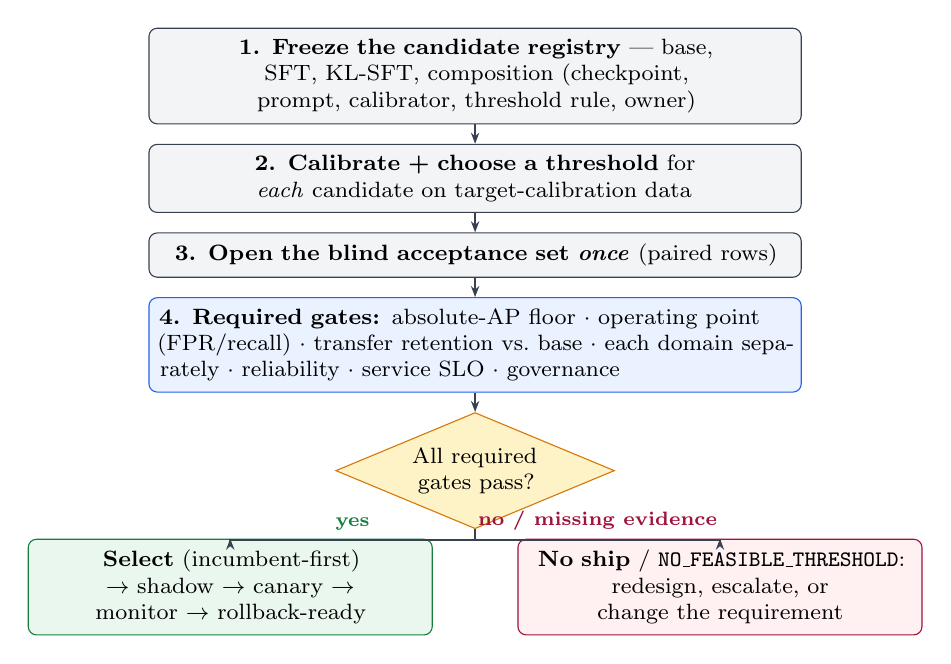
\begin{tikzpicture}[font=\footnotesize,node distance=7pt and 10pt,
  wfstep/.style={rounded corners=3pt,draw=inkgrey,fill=cardgrey,align=center,inner sep=4pt,text width=0.66\linewidth},
  gate/.style={rounded corners=3pt,draw=bgblueedge,fill=bgblue,align=left,inner sep=4pt,text width=0.66\linewidth},
  dec/.style={diamond,aspect=2.4,draw=amberedge,fill=amberfill,align=center,inner sep=1pt,text width=1.9cm},
  ship/.style={rounded corners=3pt,draw=tkgreenedge,fill=tkgreen,align=center,inner sep=4pt,text width=0.40\linewidth},
  stop/.style={rounded corners=3pt,draw=statusred,fill=statusfill,align=center,inner sep=4pt,text width=0.40\linewidth},
  arr/.style={-{Stealth[length=4pt]},inkgrey,thick}]
  \node[wfstep] (reg) {\textbf{1. Freeze the candidate registry} --- base, SFT, KL-SFT, composition (checkpoint, prompt, calibrator, threshold rule, owner)};
  \node[wfstep,below=of reg] (cal) {\textbf{2. Calibrate + choose a threshold} for \emph{each} candidate on target-calibration data};
  % \textsc inside \textbf asks for a bold small-caps shape Latin Modern does not have, which
  % emitted a font-substitution warning on every build. Emphasise with italics instead.
  \node[wfstep,below=of cal] (blind) {\textbf{3. Open the blind acceptance set \emph{once}} (paired rows)};
  \node[gate,below=of blind] (gates) {\textbf{4. Required gates:} absolute-AP floor $\cdot$ operating point (FPR/recall) $\cdot$ transfer retention vs.\ base $\cdot$ each domain separately $\cdot$ reliability $\cdot$ service SLO $\cdot$ governance};
  \node[dec,below=of gates] (q) {All required gates pass?};
  \node[ship,below left=14pt and -10pt of q] (ship) {\textbf{Select} (incumbent-first) $\to$ shadow $\to$ canary $\to$ monitor $\to$ rollback-ready};
  \node[stop,below right=14pt and -10pt of q] (stop) {\textbf{No ship} / \texttt{NO\_FEASIBLE\_THRESHOLD}: redesign, escalate, or change the requirement};
  \draw[arr](reg)--(cal); \draw[arr](cal)--(blind); \draw[arr](blind)--(gates); \draw[arr](gates)--(q);
  \draw[arr](q.south) -- ++(0,-4pt) -| (ship.north) node[pos=0.25,above,font=\scriptsize\bfseries,text=tkgreenedge]{yes};
  \draw[arr](q.south) -- ++(0,-4pt) -| (stop.north) node[pos=0.25,above,font=\scriptsize\bfseries,text=statusred]{no / missing evidence};
\end{tikzpicture}
\caption{\textbf{Gate candidates, not leaderboards} (recommended workflow; not validated end to end by
this study). Every candidate is calibrated and thresholded separately, evaluated once on a blind
acceptance set, and must clear \emph{all} required gates; a missing required gate is a failure, and an
empty feasible set is a deliberate \textsc{no-ship}, not a relaxed cutoff.}
\label{fig:gating}
\end{figure}

\subsection{Latency and cost: the case for a small, self-hosted guard}
\label{sec:practitioner-cost}
An inline guard runs on \emph{every} request, so its own latency and cost sit on the critical path.
Because our guard emits a single verdict token --- one forward pass, no autoregressive generation --- it
is fast to run: measured per-call latency is $\approx$10--50\,ms (P50--P90, batched on one A100; P99 up to $\approx$94\,ms, and composition adds a pass) depending on model size
(\Cref{tab:latency}), from $10.4$\,ms (P50) for Qwen2.5-1.5B to $25.2$\,ms for Qwen3-4B, with P90 within
$\approx$50\,ms, on a single A100 at batch~16. Latency tracks model size and prompt length, not any decode
budget, because there is nothing to decode. One caveat on reading these numbers: they are \emph{batched}
per-row times (batch~16 on one A100) --- throughput-latency under load, not a single-request, batch-1
serving path, which carries a higher fixed per-call overhead but no queueing. Treat them as an
order-of-magnitude serving estimate on this hardware, not a single-request SLA.

\input{generated/latency_table}

A frontier hosted-API guard is disadvantaged on the two axes that decide an inline deployment, and here
that is \emph{measured} rather than sketched: \Cref{tab:frontier-serving} reports hosted P50/P99 latency
and \$/1k taken on the ExpGuard rows themselves at concurrency 200, against the committed batched-A100
figures in \Cref{tab:latency}. The hosted path adds a network round-trip --- \FrontierBestMedianMs\,ms
median against tens of milliseconds --- to \emph{every} request; it bills a per-token fee that scales
with traffic; and, decisively for a regulated domain, it sends every prompt to a third party.
\Cref{tab:deployment} sets the four axes side by side.

That is a case for self-hosting the traffic you can serve well, not for self-hosting everything.
\Cref{sec:actIII-h2h} shows the accuracy ordering inverts by regime, and \Cref{sec:frontier-licenses}
prices a selective cascade that keeps the median request local. So the practical conclusion is a routing
conclusion: build from small checkpoints, and escalate the slice they serve worst --- which is what
Row~8 of \Cref{tab:guidelines} says, and what the unconditional reading of Row~6 would miss.

\begin{table}[htbp]\centering\small
\caption{Deployment economics of an \emph{inline} guard: a small self-hosted guard versus a frontier
hosted-API guard. Both columns are \emph{measured} in this study --- the small-guard latency in
\Cref{tab:latency}, the hosted latency and \$/1k in \Cref{tab:frontier-serving}, the latter on the
ExpGuard rows at concurrency 200 and therefore a throughput-regime upper bound on an isolated request
rather than a single-request figure. An earlier version of this caption described the frontier column as
an illustrative sketch ``not a measurement made here,'' which contradicted \Cref{tab:frontier-serving}.}
\label{tab:deployment}
\begin{tabular}{@{}>{\raggedright\arraybackslash}p{0.20\linewidth} >{\raggedright\arraybackslash}p{0.36\linewidth} >{\raggedright\arraybackslash}p{0.36\linewidth}@{}}
\toprule
 & Small self-hosted guard (this report) & Frontier hosted-API guard \\
\midrule
Per-call latency & one local forward pass, $\approx$10--50\,ms (\Cref{tab:latency}) & network round-trip to a hosted API, typically $10^{2}$--$10^{3}$\,ms \\
Marginal cost / call & only amortized local compute --- a 1.5--4B model serves on a commodity GPU (or CPU) & a per-token fee on every request, at the vendor's list price \\
Data residency & regulated prompts never leave your boundary & every request is sent to a third party --- a data-governance / compliance concern \\
Operational coupling & self-contained; pinned, versioned, auditable in-house & external availability, rate limits, and silent model updates \\
\bottomrule
\end{tabular}
\end{table}


% limitations/ledger/roadmap moved to Appendix E (result-specific caveats live in the E/D/B boxes)
\section{Reproducibility}
\label{sec:repro}
Every table and figure above is \code{\textbackslash input} from a committed generated artifact; the
remaining in-prose values are transcribed from those same artifacts and are not covered by the
byte-check. Two entry points, run in \code{papers/unified-report/} and both calling \code{reproduce.py}
(distinct from the repo-root \code{make repro}, which re-verifies the release cache):
\code{make regenerate} rewrites the generated artifacts from committed per-row scores, and
\code{make verify} recomputes them into a scratch directory and asserts byte-identity with the
committed copies, leaving the tracked tree byte-clean. \code{make verify} is the one a reader should
run. Read its exit code carefully, because a clean checkout does not exit $0$: it exits nonzero if any
covered artifact \emph{mismatches} \textbf{and also} if any artifact could not be checked at all. On an
ordinary machine the \ReproNEnvGated{} Act~I artifacts fall in the second bucket, so the run ends
\code{CHECK INCOMPLETE} with a nonzero status while reporting \code{0 failed}; the per-artifact table it
prints, not the exit code, is what says whether anything drifted. Only the lock-pinned environment
(\code{docs/reproducibility-environments.md}) can exit $0$. One limit is measured rather than
assumed: three \emph{upstream} generators are not redirected to the scratch directory and rewrite
their intermediates in place (the composition pilot's \code{generated/}, and the mortgage
\code{out\_eval/} and \code{generated/}). The tree still ends byte-clean, because with no drift the
rewrite is byte-identical --- but drift in one of \emph{those} intermediates would be silently
repaired rather than reported. Every artifact this report \code{\textbackslash input}s is compared
properly; the gap is one level upstream of them, and closing it needs an output-directory flag on one
script.

\textbf{Coverage is now complete, and the harness is what says so}: of the \ReproNInputs{} generated
artifacts the report \code{\textbackslash input}s, \ReproNVerified{} are byte-checked in any
environment, the remaining \ReproNEnvGated{} require the lock-pinned environment (Act~I's own tables
and the \code{\textbackslash Rep*}/\code{\textbackslash Transfer*} macros), and
\ReproNUncovered{} are uncovered. Earlier revisions left eleven inputs outside the harness ---
including \emph{both} head-to-head outputs, which back the report's most prominent frontier claim ---
and said ``every table is byte-checked'' anyway. The denominator is defined in the emitted macro file
itself: it counts every
\code{generated/*.tex} the report inputs \emph{except} \code{repro\_macros.tex}, which is the harness's
own coverage report and would make the count self-referential
(\ReproNInputsInclSelf{} files including it). Every count in this paragraph is emitted by the harness
(\code{\textbackslash Repro*}) because they were previously typed by hand and went stale twice: an
earlier version of the abstract quoted ``12 of the 24'' after the surface had grown past it, and a
later one quoted ``8 uncovered'' while the harness was emitting eleven.

\paragraph{What the previous revision could not verify, and what changed.} A prior version of this
section conceded three defects and left them open; all three are now closed, and the concessions are
kept here so the record shows what the numbers above are worth. \textbf{(i)} Eleven generated inputs sat
outside the harness --- the adaptation, KL-SFT, ensembling, cascade, mortgage-composition and, most
seriously, \emph{both} head-to-head outputs, which back the report's most prominent frontier claim. All
of their emitters read committed analysis JSON, so there was never a reason they could not be checked;
they are now wired in, and the report no longer says ``every table is byte-checked'' while its headline
table is uncovered. \textbf{(ii)} Figures were regenerated and never compared. The eleven plotted
figures are now rendered into a scratch directory and byte-compared like everything else. Two classes
sit outside that, and both are named rather than implied: the three Graphviz diagrams
(\Cref{fig:design,fig:splits,fig:pipeline}) are rendered from committed \code{.dot} sources but are not
byte-compared, because \code{dot} output is not reproducible across Graphviz builds; and
\Cref{fig:plane} ships as a committed \code{specialization\_plane.pdf} with \emph{no} generator in
\code{make\_figures.py} at all, so it is neither regenerated nor compared. It predates the harness, and
re-deriving it from \Cref{tab:seed-values} --- which holds the twenty points it plots --- is a stated
gap (\Cref{sec:roadmap}). \textbf{(iii)} Verification was not
side-effect-free: \code{make reproduce} did not pass \code{-{}-check}, and even the checking path
rewrote \code{repro\_macros.tex} --- the one artifact it never checked. Emitters now honour a
\code{PAPER\_GEN\_DIR} redirect, the coverage macro is checked like any other input, and a verification
run leaves the working tree byte-clean.

One limit is \emph{not} closed and should not be read as if it were. Re-deriving the head-to-head
artifact (\code{h2h.json}) runs a 2{,}000-replicate joint bootstrap that takes
minutes, so it is an opt-in target (\code{make verify-heavy}) rather than part of the default check.
What changed is that it is now \emph{possible} offline at all: the provider's per-row predictions were
previously reachable only through \code{gpt-baseline/raw/}, which is gitignored, so a clean checkout
could not reconstruct the head-to-head numbers by any route. They are now materialised as a committed,
text-free per-row artifact (\code{frontier\_rows.json}: content digests, the provider's 0--100 risk per
row, per-config parse/failure tallies, and the run's model string, prompt-contract digest and run id),
which the evaluator reads with \code{-{}-offline}. Labels and evaluation families come from the
committed score parquet on both paths, so the offline reconstruction cannot drift from the live one.
The matched-false-alarm-budget table (\Cref{tab:matchedfpr}) is one of the covered artifacts: it is
derived from the same committed \code{score\_raw}/\code{gold} columns as everything else here and needs
no GPU.

\paragraph{Three reproducibility tiers, kept distinct.} \textbf{(i) Analysis reproducibility} --- regenerating
a table from the committed per-row scores --- is what \code{make verify} checks byte-for-byte, with no
GPU and no network. It is the tier the \ReproNVerified{} covered artifacts meet in any environment and the
\ReproNEnvGated{} Act~I artifacts meet under the pinned lock. No input the report
\code{\textbackslash input}s now falls outside it.
\textbf{(ii) Training/scoring reproducibility} --- re-deriving those per-row scores by training the $4\times5$
adapters and rescoring --- requires a GPU and pinned model/data access (only re-scoring the gated ExpGuard
set additionally needs dataset access). \textbf{(iii) Artifact-generation reproducibility} --- regenerating
the mortgage benchmark itself --- is \emph{not} claimed: its LLM construction stages run at nonzero
temperature and the set is intentionally frozen, so only its \emph{evaluation} reproduces, not its
generation. Raw third-party rows are referenced by pinned identifier + revision + content hash, not
redistributed.

\paragraph{Benchmark attribution.} \begin{sloppypar}The worked case study of \Cref{fig:casestudy}
quotes rows of \textbf{MortgageGuardBench \code{v1\_hmda2022}}, Reza Rahimi, PhD (JazzX AI), licensed
\href{https://creativecommons.org/licenses/by/4.0/}{CC BY 4.0} --- the attribution that licence
requires, and the same notice the HTML edition carries. Its prompts are synthetic and its labels are
LLM-judge and policy-card-consistent, \emph{not} SME-adjudicated; its release checksums cover release
bytes only, not the generator, judge, configuration, or code. The prompts solicit policy violations by
design, so reuse should treat them as harmful-content samples. The factual grounding is the public HMDA
2022 loan-level snapshot, a U.S.\ Government work carrying no U.S.\ copyright. Redistribution decisions
for every source live in \code{benchmarks/registry/distribution.yaml}.\end{sloppypar}

\paragraph{Code and data availability.} \begin{sloppypar}All code, data manifests, generated tables, and
the frozen benchmark are public at \url{https://github.com/rrahimi-uci/safety-guard-dynamics}. The
one-command pipeline is \code{papers/unified-report/reproduce.py} (\code{make verify} for a non-mutating
check; \code{make regenerate} to rewrite generated artifacts); the frozen,
dual-labeled mortgage benchmark ships at \code{mortgage-benchmark/benchmark/v1\_hmda2022/} (994 rows,
SHA-256-checksummed, with a text-free index); the committed per-row guard scores that regenerate every
number live under \code{artifacts/} (the Act~I/II scores in \code{artifacts/paper\_a\_sft\_v2/}, the
mortgage baseline in \code{mortgage-benchmark/out\_eval/}, and the finance/health/law scores in
\code{artifacts/expguard\_external/}); and every figure except \Cref{fig:plane} is built by
\code{papers/unified-report/figures/make\_figures.py} (that one exception is committed without a
generator, as \Cref{sec:repro} records).\end{sloppypar}

\section{Conclusion}
\label{sec:conclusion}

Benchmark gains do not guarantee transfer. On this fixed panel, paired same-checkpoint comparisons show
a large represented-source gain ($\RepDelta$) beside heterogeneous held-out effects
($\TransferDelta$): one weak base improves, while the strongest bases lose transfer. At an equal
false-alarm budget the ambiguity disappears operationally --- transfer recall falls
$\MatchedTransferBase\!\rightarrow\!\MatchedTransferSft$ and \code{HarmBench} recall falls
$\MatchedHarmBase\!\rightarrow\!\MatchedHarmSft$, with the tuned guard worse on all four checkpoints.

The extensions sharpen the boundary rather than erase it. Released purpose-built guards move in the
same direction in a non-confirmatory fixed-panel analysis. KL-regularized SFT retains transfer only by
giving back represented gain, while base-plus-adapter composition recovers transfer for an additional
inference pass. None of these results licenses the claim that fine-tuning always harms transfer or that
one guard is universally best.

The deployment result is therefore conditional on traffic. A hosted frontier model leads on unfamiliar,
expert-annotated prompts; the tuned local panel leads on represented sources. A regulated domain adds a
second boundary: general-safety scores do not identify policy violations that read as ordinary text, so
domain-specific instruments and expert validation remain necessary.

The practical rule is the paper's final deliverable: compare every tune with its own base, on identical
represented and held-out sources, at a matched false-alarm budget; require domain, calibration, service,
and governance gates before deployment. The evidence remains retrospective except where explicitly
labelled otherwise, and the mortgage labels are not expert-adjudicated. The contribution is a workflow
that makes specialization visible before it becomes a production failure --- not a new winning model.

\clearpage
\appendix
\section{Related work}
\label{sec:related}

This report sits at the intersection of five literatures: the design of small LLM-based
\emph{guard classifiers}; the growing evidence that \emph{fine-tuning degrades} or narrows a
model's safety behavior; the study of \emph{calibration and operating points} for moderation;
\emph{model composition} in weight versus output space; and the emerging work
on \emph{domain-specialized guarding} in regulated verticals. We review each in turn and, for each,
name precisely what it establishes and what our paired, same-checkpoint,
composition-aware, four-domain design adds. Our contribution is not a new model, metric, or training
algorithm --- it is a measurement discipline and four evaluation instruments applied to one fixed
panel, so the contrast throughout is methodological rather than a claim of superior scores.

\begin{background}{How to read this map (for the non-expert)}
Almost all of the ``guard'' papers below ask \emph{how good is model $X$?} and answer with a single
benchmark number, usually next to a table of \emph{other} models. That is a \emph{leaderboard}
question. This report asks a different, paired question: \emph{what did the fine-tune change relative
to the same model before tuning, and does that change survive on data the guard never saw?} Keep that
distinction in mind --- most gaps we point to are gaps between a leaderboard number and a paired,
regime-split delta, not disagreements about which model is ``best.''
\end{background}

\subsection{Small LLM guard classifiers}
\label{sec:related-guards}
The dominant deployment pattern is a compact decoder LLM turned into a binary or taxonomy-tagged
moderation head. Llama Guard \citep{inan2023llamaguard} introduced the input--output
safeguard framing and a safety taxonomy, and later iterations pushed toward smaller, cheaper, and
multimodal variants \citep{meta2024llamaguard2,meta2024llamaguard3_8b,meta2024llamaguard3_1b,%
fedorov2024llamaguard3_1b,meta2025llamaguard4}. ShieldGemma \citep{zeng2024shieldgemma} and Granite
Guardian \citep{padhi2024graniteguardian} extend the recipe to other base families with broad harm
taxonomies; WildGuard \citep{han2024wildguard} adds one-stop coverage of prompt harm,
response harm, and refusal detection; and Qwen3Guard \citep{qwen3guard2025} is a recent open guard on
the same Qwen family two of our checkpoints come from. Beyond the general-purpose guards, several works
target narrower slices or richer inference: dedicated prompt-injection detectors
\citep{meta2024promptguard,meta2025promptguard2_86m,meta2025promptguard2_22m}, reasoning- and
logic-augmented guardrails \citep{kang2025r2guard}, ensemble-of-experts moderation
\citep{ghosh2024aegis}, RL-driven multilingual guardrails \citep{deng2025duoguard}, and CPU-class or
multi-stage pipelines aimed at cost \citep{majhi2025gpuguard}. The parameter-efficient adaptation we
use --- LoRA \citep{hu2021lora} applied to a chat model to produce a guard --- is exactly the LoRA-Guard
recipe \citep{elesedy2024loraguard}, and standardized suites such as GuardBench
\citep{bassani2024guardbench} have made cross-model comparison routine.

What this family reports, almost without exception, is \emph{absolute} moderation performance of
\emph{one} guard against \emph{different} models on a benchmark. That is precisely the quantity we argue
is co-produced by the benchmark and therefore uninformative about a specific fine-tune. Several of these
works do report in-distribution versus out-of-distribution blocks --- Llama~Guard's own test set against
zero-shot ToxicChat and OpenAI-Mod, WildGuard's and LoRA-Guard's ID/OOD splits --- so the
represented/transfer \emph{distinction} is not ours. Our narrower claim, stated once and not widened
anywhere else in this report, is:

\begin{quote}
a same-checkpoint \emph{paired} measurement of LoRA-induced change across represented and
source-held-out regimes, together with a calibrated base-plus-adapter composition test under matched
false-alarm budgets.
\end{quote}

\noindent An earlier version of this passage said instead that ``none of them reports'' the paired
change and that ``none treats retraining-free composition as a measurable design axis.'' Both were
overclaims that survived because the comparison was made in prose rather than against a table; the
per-component comparison in \Cref{tab:closest} is what replaces them. We reuse the LoRA-Guard recipe not to beat
these guards on a leaderboard --- we score four small open checkpoints, not the gated production guards
--- but to isolate what the fine-tune itself does. GuardBench and its peers are the backdrop against
which \Cref{sec:actI}'s question is posed: they normalize the single-suite comparison whose fragility we
show is fragile.

\subsection{Fine-tuning degradation and policy / benchmark transfer}
\label{sec:related-transfer}
The closest prior evidence is that fine-tuning can \emph{weaken} rather than strengthen safety.
\citet{hsiung2025guardrails} show that safety guardrails can collapse after fine-tuning and attribute
the collapse to similarity between the alignment and fine-tuning data --- a mechanism that rhymes with
our specialization finding, but is measured on a model's own alignment behavior rather than on a guard
classifier's represented-versus-transfer ranking split. \citet{liu2026domaingeneralizable} document that
guardrails overfit their training \emph{policy} and propose augmented policy training as a remedy;
\citet{li2026surfaceheuristics} give a complementary mechanistic account, showing that prompt-attack
defenses learn \emph{surface heuristics} that do not generalize --- essentially a why for the transfer
loss we observe empirically. \citet{bassani2025robustness} probe the same fragility from the
perturbation side, measuring guardrail robustness to input mutations and adversarial attacks, and
\citet{hackett2025bypassing} demonstrate concrete evasion of injection/jailbreak detectors. Framed most
generally, \citet{akinrele2026regime} argue that prompt-injection detection is \emph{regime-dependent} ---
performance is a function of the deployment regime, not a fixed model property --- which is our thesis
stated for one task with interpretable structural signals.

Our addition is the measurement design rather than the qualitative claim. Where these works compare a
model before and after, or one policy against another, we hold the \emph{checkpoint, manifest, seeds,
and scorer fixed} and read the paired change as a distribution over a purposively chosen panel with a
hierarchical bootstrap, and we decompose it into a large represented-source gain versus a near-flat but
\emph{heterogeneous} transfer change (\Cref{tab:primary}, \Cref{fig:plane}). Crucially, we do not stop
at ``degradation'': we quantify the specialization geometry per checkpoint and per benchmark, carry it
to a deployable operating point (\Cref{tab:sensitivity}), and then ask whether a composition
(\Cref{sec:actIII}) changes it. And unlike \citet{liu2026domaingeneralizable}, whose remedy retrains with
augmented policies, our candidate remedy retrains nothing.

\subsection{Calibration and operating points}
\label{sec:related-calibration}
Ranking quality (average precision) and thresholded decision quality are distinct, and the gap between
them is a calibration problem. \citet{guo2017calibration} established that modern neural networks are
systematically miscalibrated and that simple post-hoc scaling helps; \citet{liu2025calibration}
specialized this to LLM-based guard models, showing they are poorly calibrated for reliable content
moderation; and FlexGuard \citep{flexguard2026} moves past a single fixed threshold toward continuous,
strictness-adaptive risk scoring. This literature motivates two choices we make: we fit calibrators only
on a development split before reading any threshold, and we report operating-point behavior (macro- and
pooled-FPR, TPR, single-class recall) \emph{separately} from ranking.

Our specific contribution to this thread is a clean separation of the two failure modes on the \emph{same}
guards. In Act~II we show that a composition can recover transfer \emph{ranking} while its realized
false-alarm rate at a fixed FPR target still misses (\Cref{tab:pilot-operating}): recovering rank does
not deliver a transferable threshold. In Act~III the same lesson recurs from the other direction --- for
tightly clustered guard scores the fixed-threshold operating point is knife-edge and unstable across
software versions, which is why we deliberately do not tabulate it there. Where the calibration
literature asks ``is this score a probability?'', we use that machinery to make the sharper point that
\emph{ranking recovery $\neq$ calibration transfer}, a distinction a benchmark AP number alone hides.

\subsection{Weight-space versus output-space composition}
\label{sec:related-composition}
Combining models to improve robustness under distribution shift is well studied in \emph{weight} space:
WiSE-FT interpolates a fine-tuned model with its zero-shot initialization \citep{wortsman2022wiseft},
and model soups average the weights of several fine-tunes \citep{wortsman2022modelsoups}, both trading a
little in-distribution accuracy for out-of-distribution robustness at no extra inference cost. The
theoretical companion most relevant to us is \citet{kumar2022calibrated}, who show that \emph{calibrated
ensembles} --- combining models in \emph{output} space after calibration --- can mitigate the
accuracy--robustness tradeoff under shift; this is the justification behind our composition rule.

Act~II (\Cref{eq:comp}) is deliberately the output-space cousin of these methods: we average the
base's and the adapter's \emph{calibrated scores} with fixed equal weights, retraining nothing. The
tradeoff versus WiSE-FT/soups is explicit --- output-space composition needs only comparable scores,
not interpolable weights, so it is portable across checkpoints that could never be weight-averaged, but
it pays for two inference passes. We position composition as a \emph{transfer-recovery remedy for guard
specialization} specifically (represented cost small, transfer recovered relative to SFT and landing
above base; \Cref{tab:pilot-summary,tab:pilot-models}), and we are explicit about what the pilot does
\emph{not} include --- an actual WiSE-FT weight-space rescoring is
left as a control in the roadmap, and the logit-average variant is reported only as a non-promotable
ablation. The equal-cost SFT+SFT control \emph{is} run (\Cref{tab:sftsft}): base+SFT beats SFT+SFT on every
checkpoint, so the transfer recovery is attributable to keeping the base rather than to generic two-model
ensembling. To our knowledge this calibrated output-space average has not been evaluated as a targeted fix
for the represented/transfer split in small safety guards.

\subsection{Domain-specialized guarding and regulated verticals}
\label{sec:related-domain}
A recent line moves guarding from generic harm to \emph{domain compliance}. ExpGuard
\citep{expguard2026} provides expert-annotated content moderation in specialized domains including
finance, health, and law --- we adopt it directly as our external, expert-labeled breadth replication
(\Cref{tab:expguard}; complete four-checkpoint base result). FinGuard
\citep{dou2026finguard} detects financial regulatory non-compliance in LLM interactions; MortarBench
\citep{toles2026mortarbench} evaluates mortgage loan-origination \emph{agents}; and
\citet{bowen2024mortgage} measure and mitigate racial bias in LLM mortgage \emph{underwriting}.
Adjacent security-benchmark methodology such as Gate AI \citep{goehausen2026gateai} rounds out the
evaluation-design context, and our mortgage instrument is grounded in public HMDA loan-level data
\citep{hmda2022}.

Each of these captures one facet our four-domain design tries to unify while keeping the honesty stance
explicit. FinGuard is single-domain and, like the general guards, reports absolute detection rather than
a paired base-versus-tuned transfer delta. MortarBench evaluates whether an \emph{agent completes} an
origination task, not whether a \emph{guard detects} a compliance violation, and it does not isolate the
requests that read as safe yet violate policy. \citet{bowen2024mortgage} study bias in the model's own
underwriting \emph{decisions}, whereas we study a guard's \emph{detection} behavior and add a
protected-class \emph{minimal-pair} invariance gate as a fairness signal that ranking alone misses. Our
mortgage benchmark's distinctive construct is the \emph{dual label} $G\times D$ (\Cref{tab:composition},
\Cref{fig:pipeline}), whose load-bearing G0/D1 stratum --- looks safe, is a violation --- is exactly the
case a general-safety score cannot see; the zero-shot baselines (\Cref{tab:baseline}) show these
compliance violations are only moderately ranked even by the strongest base. Two honesty boundaries
separate our instruments from the certified-audit reading a reader might infer: the mortgage labels are
\emph{LLM-judge, policy-card-consistent --- not SME-adjudicated}, and ExpGuard supplies the strictly
stronger expert-labeled tier but as a \emph{single-label} transfer probe, not a dual-label construct. We
therefore pair one domain built in depth (mortgage, dual-label plus fairness gate) with three external
verticals for breadth (finance/health/law via ExpGuard), all scored on the same fixed panel used in
Acts~I--II so the specialization question can be asked identically across domains.

% The component-by-component comparison (tab:closest) and its discussion were moved into the
% Introduction (sec:related-closest): the novelty claim is made there, so the table that bounds
% it has to be visible there too rather than 50 pages later.
\noindent The component-by-component comparison against the six closest contributions, and the
narrowed novelty statement it forces, are in \Cref{sec:related-closest} and \Cref{tab:closest} ---
placed in the Introduction beside the claim they bound.

\begin{takeaway}{The gap this report fills}
Prior work establishes, separately, that guards can be built cheaply from small LLMs, that fine-tuning can
degrade or narrow safety, that guards are miscalibrated, that weight-space averaging aids robustness, and
that regulated domains need their own benchmarks. What is missing --- and what
this report supplies on one fixed four-checkpoint panel --- is a single, reproducible, estimation-only
thread that (i) measures the fine-tune as a \emph{paired, same-checkpoint} represented-versus-transfer
delta, (ii) tests a retraining-free \emph{output-space composition} as a targeted transfer-recovery
remedy, and (iii) carries the same question across \emph{four regulated domains} with a dual-label mortgage
construct and a fairness invariance gate. We add no new model or metric; we add the discipline of asking,
at every scale, what the benchmark contributed to the verdict.
\end{takeaway}
       % Appendix A: related work (moved out of the main narrative)
% Moved from background-setup.tex (proposal: detailed methods -> appendix).
\section{The shared experimental setup}
\label{sec:setup}

Every study in this report reuses one fixed, purposively chosen panel of four checkpoints and one
frozen, decontaminated $1{,}200$-row training manifest, scored by the identical single-token
$z_{\text{unsafe}}-z_{\text{safe}}$ head (\Cref{eq:score}) and the same tie-aware macro-AP, under
fail-closed provenance \emph{locks} that bind the data, code, and software versions and refuse to run
if any fingerprint mismatches. This single-panel, single-manifest discipline is what makes SFT,
composition, and the domain evaluations \emph{directly comparable} rather than stapled
results. The \emph{same} four checkpoints recur across all three acts, and \textbf{Qwen3-4B is the
recurring character}: the strongest base, and --- as the acts will show --- the one that specializes
most, the one composition helps least, and the numerically highest-ranking, most
protected-token-invariant zero-shot mortgage guard (within overlapping CIs --- \Cref{tab:baseline}
does not license a ranking).

\subsection{The fixed four-checkpoint panel and pinned revisions}
\label{sec:setup-panel}

The panel spans two model lineages and $1.5$--$4$B parameters: Qwen2.5-1.5B-Instruct,
SmolLM2-1.7B-Instruct, SmolLM3-3B \citep{bakouch2025smollm3}, and Qwen3-4B. Each checkpoint is pinned to
a fixed upstream revision, and for each we verify that \code{safe} and \code{unsafe} map to
\emph{distinct single tokens} under a fixed convention (leading-space \code{" safe"}/\code{" unsafe"}
first, no-leading-space fallback), recording the token IDs and strings. \Cref{tab:panel-recipe} lists
the panel and the frozen recipe together. The estimand is this exact four-checkpoint panel; results are
not extrapolated to other scales, architectures, or vendors.

\begin{table}[htbp]
\centering\small
\caption{The fixed model panel and the frozen clean-v2 LoRA-SFT recipe (shared by Acts~I--II).
Revisions are pinned; decision tokens are verified as distinct single tokens per checkpoint.}
\label{tab:panel-recipe}
\resizebox{\textwidth}{!}{%
\begin{tabular}{lll l}
\toprule
Checkpoint & Params & Revision (pinned, abbreviated) & Decision tokens \\
\midrule
\code{Qwen/Qwen2.5-1.5B-Instruct}        & 1.5B & \code{989aa79\ldots71aa306}  & \{\,safe, unsafe\,\} single-token \\
\code{HuggingFaceTB/SmolLM2-1.7B-Instruct} & 1.7B & \code{31b70e2\ldots46d38674} & \{\,safe, unsafe\,\} single-token \\
\code{HuggingFaceTB/SmolLM3-3B}          & 3B   & \code{a07cc9a\ldots335b0ac1} & \{\,safe, unsafe\,\} single-token \\
\code{Qwen/Qwen3-4B}                     & 4B   & \code{1cfa9a7\ldots03b3df60c} & \{\,safe, unsafe\,\} single-token \\
\midrule
\multicolumn{4}{l}{\emph{Recipe (identical for all four bases):} completion-only SFT loss on the verdict $+$ appended EOS;}\\
\multicolumn{4}{l}{LoRA $r{=}32$, $\alpha{=}64$, dropout $0.05$ on \{q,k,v,o,gate,up,down\}; $300$ optimizer steps;}\\
\multicolumn{4}{l}{lr $2\times10^{-4}$ cosine schedule, warmup $0.03$; effective batch $4$; max sequence length $1{,}024$;}\\
\multicolumn{4}{l}{training seeds $42$--$46$ (five per checkpoint), shared data-order seed $42$.}\\
\bottomrule
\end{tabular}}
\end{table}

\subsection{The single-token guard formulation and prompt rendering}
\label{sec:setup-guard}

Every base and every adapter is scored by the same guard formulation from \Cref{sec:bg-guard}: the
prompt is wrapped in one versioned instruction template asking for a one-word verdict, and the last
position's \code{safe}/\code{unsafe} logits are read and stored as $s(x)$ (\Cref{eq:score}), with the
softmax probability (\Cref{eq:prob}) derived from them. The \emph{semantic} system instruction is
shared verbatim across all four checkpoints, but each model's own chat template renders it differently,
producing three distinct rendered-template fingerprints across the panel; each is recorded. Long user
content is budgeted and truncated \emph{before} final rendering, and the runner then asserts that the
complete classification instruction and wrapper survive the truncation --- a contract check motivated by
an earlier artifact that could left-truncate the instruction itself. Truncation strategy and scored
token counts are stored per row.

\subsection{The frozen LoRA-SFT recipe}
\label{sec:setup-recipe}

The recipe (lower panel of \Cref{tab:panel-recipe}) is fixed identically across all four bases so that
the only thing varying within Act~I is the checkpoint. It uses a \emph{completion-only} loss --- the
cross-entropy is applied only to the verdict token and an appended end-of-sequence marker, not to the
prompt --- with a LoRA adapter of rank $r{=}32$ and scaling $\alpha{=}64$ (dropout $0.05$) inserted into
the attention and MLP projections (q, k, v, o, gate, up, down). Training runs $300$ optimizer steps at
learning rate $2\times10^{-4}$ on a cosine schedule with $0.03$ warmup and an effective batch size of
$4$, at maximum sequence length $1{,}024$. At effective batch $4$, the $1{,}200$-row manifest yields
exactly $300$ updates --- one complete exposure of the data. Each base is adapted with five training
seeds ($42$--$46$) that share one data-order seed ($42$), giving $20$ adapters; the four untuned bases
are scored once and reused, for $24$ model bundles in all.

\subsection{The 1,200-row training manifest and exclusions}
\label{sec:setup-manifest}

Training reads one frozen manifest and never resamples a live dataset mid-run. It draws $400$ rows each
from three represented sources --- ToxicChat \citep{lin2023toxicchat}, Prompt-Injections, and
Jailbreak-Classification --- with $200$ safe and $200$ unsafe rows per source, selected by a hashed rank
salted with the data seed and frozen as one shared row order across every checkpoint and seed
(\Cref{tab:manifest}). Two datasets are \emph{deliberately excluded from training}: BeaverTails
\citep{ji2023beavertails}, because its safety annotation labels the prompt--response interaction rather
than the prompt alone, and OR-Bench \citep{cui2024orbench}, which is reserved for the benign stress set;
including either would confound the prompt-only, dataset-held-out design. The study uses the
non-commercial academic data branch (ToxicChat is CC BY-NC 4.0), so any released adapter inherits a
non-commercial mark, and no third-party raw text is redistributed --- only pinned identifiers,
revisions, and content hashes.

\begin{table}[htbp]
\centering\small
\caption{The frozen $1{,}200$-row training manifest (Acts~I--II). All training rows come from three
represented sources; each contributes $400$ rows balanced $200{:}200$. BeaverTails and OR-Bench are
excluded from training by design.}
\label{tab:manifest}
\begin{tabular}{l l r}
\toprule
Represented source & Native label origin & Train rows (safe : unsafe) \\
\midrule
ToxicChat (\code{lmsys/toxic-chat})           & prompt toxicity   & $400$ ($200{:}200$) \\
Prompt-Injections (\code{deepset/prompt-injections}) & prompt injection & $400$ ($200{:}200$) \\
Jailbreak-Classification (\code{jackhhao/\ldots}) & prompt jailbreak & $400$ ($200{:}200$) \\
\midrule
\textbf{Total} & & $\mathbf{1{,}200}$ ($600{:}600$) \\
\bottomrule
\end{tabular}
\end{table}

\begin{figure}[htbp]\centering
\includegraphics[width=\linewidth]{data_splits.png}
\caption{\textbf{How the training, validation, and test sets are built.} Public source datasets (left),
each pinned by identifier, revision, and content hash, pass through a decontamination and
family-isolation gate --- MinHash char-5-gram near-duplicate \emph{families} are each assigned
\emph{whole} to a single split --- yielding five disjoint sets: the $1{,}200$-row \textbf{train} manifest
(fine-tuning), a held-back \textbf{validation}/calibration split (temperature + operating point only), the
\textbf{represented-source} and \textbf{dataset-held-out transfer} test sets, and single-class
\textbf{stress} probes. No family crosses the train/test or validation/test boundary, and the build
\emph{fails closed} if one would. BeaverTails is excluded entirely (it labels the prompt--response
interaction, not the prompt).}
\label{fig:splits}
\end{figure}

\subsection{Three evaluation regimes and decontamination}
\label{sec:setup-decon}

Evaluation is partitioned into three regimes, forming a spectrum of how ``new'' each test is to the
guard (\Cref{fig:splits} shows the full construction, from sources through the family-isolation gate to
these regimes; \Cref{tab:datasets} is the complete roster of every dataset used in this report, with its
role, size, and reference).
\begin{itemize}[leftmargin=1.4em,itemsep=1pt]
  \item \textbf{Represented-source} $=$ \{ToxicChat, Prompt-Injections, Jailbreak-Classification\} rows
  \emph{held back} from training. These measure discrimination on sources the guard trained on.
  \item \textbf{Dataset-held-out transfer} $=$ \{JailbreakBench \citep{chao2024jailbreakbench}, XSTest
  \citep{rottger2024xstest}, WildGuardTest \citep{han2024wildguard}, WildJailbreak
  \citep{jiang2024wildteaming}\}, whose rows were withheld from SFT. Because these encode heterogeneous
  native constructs (harm, refusal, jailbreak, contrast), their macro-average mixes distinct policies;
  we study \emph{dataset-held-out benchmark transfer}, not one fixed universal policy.
  \item \textbf{Stress} $=$ \{OR-Bench-Hard benign portion (false-positive rate only), HarmBench
  \citep{mazeika2024harmbench} (recall only)\}. These are single-class probes: \textbf{no AP or AUROC is
  computed on stress data}; they only watch for over-blocking (benign FPR) and missed attacks (recall).
\end{itemize}
The primary metric within each regime is benchmark-macro AP; the secondary metric is the
calibration-targeted operating point of \Cref{sec:setup-stats}.

\begin{table}[htbp]
\centering\footnotesize
\setlength{\tabcolsep}{4pt}
\caption{Every dataset and benchmark used in this report, grouped by role. The three represented sources
supply both the fine-tuning manifest (400 rows each, $200{:}200$ safe:unsafe) and, on held-back rows, the
represented-source test; the transfer and stress sets are never seen in fine-tuning. Act~III adds two
regulated-domain benchmarks. All sources are consumed by pinned identifier, revision, and content hash;
``rows'' are the counts \emph{used here}, not necessarily the full upstream release.}
\label{tab:datasets}
\begin{tabular}{@{}p{0.40\linewidth} p{0.30\linewidth} p{0.12\linewidth} c@{}}
\toprule
Dataset (source) & Native task / label & Rows used & Ref. \\
\midrule
\multicolumn{4}{@{}l}{\emph{Represented sources} --- fine-tuning manifest $+$ held-back represented test} \\
ToxicChat (\code{lmsys/toxic-chat}) & prompt toxicity & 400 train & \cite{lin2023toxicchat} \\
Prompt-Injections (\code{deepset/prompt-injections}) & prompt injection & 400 train & --- \\
Jailbreak-Classification (\code{jackhhao/\ldots}) & prompt jailbreak & 400 train & --- \\
\midrule
\multicolumn{4}{@{}l}{\emph{Dataset-held-out transfer test} --- never fine-tuned on; benchmark-macro AP} \\
JailbreakBench & jailbreak robustness & held-out & \cite{chao2024jailbreakbench} \\
XSTest & exaggerated-safety / refusal & held-out & \cite{rottger2024xstest} \\
WildGuardTest & prompt harm / refusal & held-out & \cite{han2024wildguard} \\
WildJailbreak & in-the-wild jailbreak & held-out & \cite{jiang2024wildteaming} \\
\midrule
\multicolumn{4}{@{}l}{\emph{Stress probes} --- single-class; no AP/AUROC} \\
OR-Bench-Hard (benign) & over-refusal (benign FPR) & benign only & \cite{cui2024orbench} \\
HarmBench & red-team attacks (recall) & attacks only & \cite{mazeika2024harmbench} \\
\midrule
\multicolumn{4}{@{}l}{\emph{Excluded from training by design}} \\
BeaverTails (\code{PKU-Alignment/BeaverTails}) & prompt$+$response safety & --- & \cite{ji2023beavertails} \\
\midrule
\multicolumn{4}{@{}l}{\emph{Regulated-domain benchmarks} (Act~III)} \\
Mortgage \code{v1\_hmda2022} (ours) & dual $G{\times}D$ $+$ protected pairs & 994 & \cite{hmda2022} \\
ExpGuard (\code{6rightjade/expguardmix}) & finance / health / law prompt safety & 2{,}275 & \cite{expguard2026} \\
\bottomrule
\end{tabular}
\end{table}

\paragraph{Decontamination (family-isolated splits, MinHash).} To keep near-duplicate rows from
straddling the train/evaluation and calibration/test boundaries, the builder first preserves the
authoritative upstream conversation, pair, and scenario identifiers, then adds deterministic character
$5$-gram \emph{MinHash} edges between near-duplicate rows. It forms the connected components of that
graph --- ``families'' --- and assigns \emph{whole families} to a single split, so that no family can
appear in both training and any reported evaluation, or in both calibration and any reported test or
stress surface. The build \emph{fails closed} if any family crosses a forbidden boundary. This family
graph also supplies the Poisson(1) re-count weights used by the bootstrap (\Cref{sec:bg-estimand}). An
independent audit of $24$ hard assertions covers the source exclusions, schema and row identity,
exact and conflicting-label overlap, pinned revisions and content hashes, selection provenance, family
disjointness, licenses, and near-duplicate dispositions. This is a \emph{build-time} gate (family isolation
plus the $24$ assertions), and it is distinct from the \emph{formal retrospective overlap audit} of the
manifest against the current v2 transfer suite, which remains \emph{pending} (\Cref{sec:not-establish}): the
gate guarantees no near-duplicate family straddles a split within the constructed graph, but a from-scratch
n-gram / near-duplicate check of the $1{,}200$-row manifest against the v2 transfer benchmarks has not yet
been run --- and any residual overlap it found would make specialization look \emph{milder}, so this is a
caveat in the direction of caution.

\subsection{Estimands and the statistical protocol}
\label{sec:setup-stats}

For regime $R$, checkpoint $b$, and seed $r$, the per-regime metric is the equal-weight macro-AP over
that regime's benchmarks,
\begin{equation}
\label{eq:regime-metric}
M_R(b,r) \;=\; \frac{1}{|K_R|}\sum_{k\in K_R}\mathrm{AP}_k(b,r),
\end{equation}
using the tie-aware, non-interpolated \code{scikit-learn} AP. The paired base-to-tuned change for one
cell is
\begin{equation}
\label{eq:delta}
\Delta_R(b,r) \;=\; M_R(\mathrm{SFT}_{b,r}) \;-\; M_R(\mathrm{base}_b),
\end{equation}
and the fixed-panel aggregate averages the four per-checkpoint deltas \emph{without} resampling
checkpoint identities,
\begin{equation}
\label{eq:agg}
\bar\Delta_R \;=\; \frac{1}{4}\sum_{b}\Big[\tfrac{1}{5}\textstyle\sum_r M_R(\mathrm{SFT}_{b,r})
\;-\; M_R(\mathrm{base}_b)\Big].
\end{equation}
The headline object is the joint vector $\theta=(\bar\Delta_{\text{represented}},
\bar\Delta_{\text{transfer}})$, kept as a two-dimensional quantity and read off the
\emph{specialization plane} of \Cref{fig:plane} --- horizontal axis the represented change, vertical the
transfer change, four quadrants (uniform gain, specialize, uniform loss, transfer-favored) --- rather
than collapsed into a single ``specialization score.'' The axes and quadrant interpretation are
result-independent.

\paragraph{Uncertainty.} We attach $95\%$ two-sided intervals with $10{,}000$ paired
hierarchical-bootstrap replicates (fixed RNG seed $20260712$): checkpoint identities are held fixed, SFT
seed indices are resampled \emph{within} each checkpoint, and one Poisson(1) weight is drawn per
recorded family (\Cref{sec:setup-decon}). Leave-one-checkpoint-out and leave-one-transfer-benchmark-out
values are \emph{deterministic} sensitivity checks, not resampling or population inference. The locked
analysis mode is \emph{precision-focused}: we report estimates, intervals, and sensitivities, with no
intersection--union test, multiplicity correction, bootstrap $p$-value, or pass/fail gate.

\paragraph{Calibration-only operating point.} As a secondary deployment diagnostic, we fit one positive
temperature per bundle on the calibration split, then choose the threshold that maximizes calibration
recall subject to a one-sided $95\%$ Clopper--Pearson \emph{upper} bound of at most $5\%$ on pooled
calibration-negative FPR; if no cutoff qualifies, the cell reports \code{NO\_FEASIBLE\_THRESHOLD} as an
outcome rather than relaxing the target. Temperature and threshold are fit \emph{only} on calibration
rows --- never on transfer or stress data --- and the audit hard-asserts that calibration shares no
family with any reported test or stress surface. The Clopper--Pearson bound assumes independent
Bernoulli negatives, so it is a pooled diagnostic, not a family-aware production guarantee. The
resulting operating-point rates appear in \Cref{tab:sensitivity} (Act~I) and \Cref{tab:pilot-operating}
(Act~II).

\subsection{The composition protocol}
\label{sec:setup-composition}

Act~II's remedy needs no retraining. For a single input we run the base and one SFT adapter, convert
each raw score to a probability with a calibrator fit only on a development split, and report the fixed
equal-weight average defined later as \Cref{eq:comp}. The $\tfrac12$ weights are fixed in advance (never
tuned on test rows), so the only cost is the second inference pass. This is the output-space composition
of \Cref{sec:bg-composition}; the logit-average and convex-weight variants were visible during
development and are reported only as non-promotable ablations.

\subsection{Domain evaluation instruments: mortgage and ExpGuard}
\label{sec:setup-domain}

Act~III evaluates the \emph{same four checkpoints} on two complementary regulated-domain instruments.

\paragraph{Mortgage (built in depth, dual-label).} We constructed a fixed, HMDA-grounded benchmark whose
unit is one incoming request carrying two independent labels, general-safety $G$ and mortgage-policy $D$
(\Cref{sec:bg-mortgage}). Requests are grounded in de-identified, banded HMDA fact sheets --- never
verbatim records --- through an agentic pipeline that plans, grounds, generates, adversarially mutates,
and rubric-bound-judges each item, accepting it only if its assigned label matches the target, before a
provenance-tracked, family-isolated split into the frozen release (\Cref{fig:pipeline}). The benchmark
has $994$ rows over four $G\times D$ quadrants --- G0/D0 ($450$), G0/D1 ($502$), G1/D1 ($42$), and G1/D0
($0$, empty by construction) --- with the load-bearing \textbf{G0/D1} stratum (reads safe, is a
violation) the largest. It spans seven content strata (fair-lending $204$, fraud $112$, UDAAP $90$,
disclosure $66$, ATR/QM $54$, privacy $18$, and benign $450$) and is split into train $604$ / dev $149$
/ public-test $146$ / private-test $95$. As a fairness-invariance gate it embeds $39$ protected-class
\emph{protected pairs} ($78$ rows) differing only in the protected attribute, of which $21$ are
true single-token swaps and the rest substitute a longer phrase (\Cref{sec:actIV-mortgage-pairs}); the induced
prediction gap is denoted $\Delta_{\text{context}}$. The row composition is in \Cref{tab:composition} and
the zero-shot base results (AP$\cdot$G, AP$\cdot$D, $\Delta_{\text{context}}$) in \Cref{tab:baseline}
(Act~III).

\begin{takeaway}{A measuring stick, not a legal finding}
Mortgage labels are assigned by an \emph{LLM judge} against written policy cards --- \emph{not}
SME-adjudicated (self-consistency only; no human Fleiss-$\kappa$). The G1/D0 quadrant is empty and some
strata are small. The benchmark \emph{surfaces} guard behavior; it certifies nothing about any real
lender or model, and licenses no fair-lending claim.
\end{takeaway}

\paragraph{Finance, health, law (external breadth: ExpGuard).} To test whether the
specialization/transfer pattern recurs across regulated verticals \emph{with expert labels} --- a
strictly stronger labeling tier than the mortgage LLM-judge --- we also score the same four checkpoints
on ExpGuard \citep{expguard2026}, an expert-annotated moderation set of $2{,}275$ rows spanning
\textbf{finance}, \textbf{health}, and \textbf{law}, using its \code{prompt\_label} for input-prompt
classification (matching our task). This is a single-label transfer probe, not the mortgage dual-$G\times D$
construct --- one domain built in depth plus three external verticals for breadth. We report aggregate
and per-domain AP for the four base checkpoints (\Cref{tab:expguard}, \Cref{fig:expguard-domains}). The
four-checkpoint result is complete and reproducible from committed text-free per-row scores; the tuned
comparison is future work.
   % Appendix B: shared experimental setup, frozen objects, statistical protocol
% Appendix C: full construction + mechanism detail (moved from the main narrative).
\section{Benchmark construction and mechanism detail}
\label{app:detail}

\subsection{The attractor: post-SFT scores are benchmark-fixed, so ``stronger bases specialize more'' is arithmetic}
\label{sec:actI-coupling}

The cleanest way to see what Act~I does and does not show is to notice a regularity that runs underneath
\Cref{tab:primary}: \textbf{fine-tuning behaves like an attractor}. No matter where a checkpoint starts,
SFT pulls its ranking to nearly the \emph{same} score on a given benchmark. Represented-source AP after SFT
is $0.982 \pm 0.005$ across the four checkpoints; transfer AP after SFT is $0.807 \pm 0.024$ --- both far
tighter than the \emph{base} spread they came from ($0.178$ and $0.073$ respectively; the transfer variance
shrinks about \textbf{9-fold}). \Cref{fig:attractor} (left) shows the collapse: four widely spread base
scores, one narrow post-SFT band.

\begin{figure}[htbp]\centering
\includegraphics[width=0.99\linewidth]{fig_attractor.pdf}
\caption{\textbf{The fine-tuning attractor.} \emph{Left:} on the transfer benchmarks the four base
checkpoints span $0.79$--$0.94$ macro-AP, but after SFT they collapse into a narrow band around a
benchmark-fixed endpoint $A_T\approx0.81$. \emph{Right:} because every checkpoint lands near that same
endpoint, the paired change $\Delta=\text{SFT}-\text{base}$ is forced onto a line of slope $-1$ (green);
the four points sit on it (fitted slope $-1.05$, $R^2=0.91$). ``Stronger bases specialize more'' is
therefore arithmetic, not a discovered behavioral law.}
\label{fig:attractor}
\end{figure}

\paragraph{Why this reframes ``stronger bases specialize more.''} Once the endpoint is (approximately)
fixed, the change we plot is pure subtraction: $\Delta = \text{endpoint} - \text{base}$. A stronger base
then \emph{must} show a smaller $\Delta$ --- not because strong models are intrinsically fragile, but
because they start closer to the ceiling. This is testable. Regressing $\Delta$ on the
base score across the four checkpoints gives slope $-0.99$ (represented, $R^2=0.999$) and $-1.05$ (transfer,
$R^2=0.91$) --- the $-1$ the attractor \emph{predicts before any fitting}. One caveat on reading those
numbers: the represented $R^2=0.999$ is close to \emph{definitional}. When the endpoint band is as tight as
it is on represented sources ($\pm0.005$), $\Delta=\text{endpoint}-\text{base}$ is arithmetically almost a
slope-$-1$ line in the base score, so a near-perfect fit is nearly forced and is not independent
confirmation of anything. The transfer fit, where the endpoint band is several times wider, is the
load-bearing test --- and it still lands at slope $-1.05$. Either way the eye-catching ordering
(SmolLM2 $+0.040$ down to Qwen3-4B $-0.150$) carries no behavioral content beyond the endpoints themselves.

\paragraph{Where the real content lives.} Two places, both benchmark-owned rather than model-owned. First,
\emph{where the endpoints sit}: $A_T\approx0.81$ is largely a property of the \emph{(training manifest,
benchmark)} pair --- to the precision of the small residuals below, the base model has largely dropped out
of the equation, and the post-SFT score is \emph{largely determined by} the manifest and the benchmark
rather than by which checkpoint you started from. This is the mechanism behind the title's claim:
after SFT the score is largely a property of the (manifest, benchmark) pair, so a gain measured on that
pair says correspondingly little about any other. Second, the \emph{small residuals} around the
endpoint (at most $0.027$ on transfer): these measure how much of a base's identity survives the fine-tune,
and are arguably a more honest per-checkpoint quantity than $\Delta$ itself. LoRA only adds a low-rank
correction in the base's own features, so full base-independence is approximate by construction --- the
residual is exactly that approximation, made visible.

\begin{background}{Why the represented ceiling is $\approx0.98$, not $1.0$ --- and why that helps the thesis}
A ranker of the \emph{latent} truth generally cannot score AP $=1$ against slightly noisy \emph{observed}
labels (though it can rank the observed labels perfectly if the noise is systematic and learnable): under
random label noise a small rate $\eta$ of ambiguous or mislabeled rows lowers the expected achievable AP to
roughly $1-1.3\,\eta$ (the coefficient
$1.3$ is an order-of-magnitude rule of thumb, not derived here --- the exact factor depends on prevalence
and on where mislabels fall in the ranking). The observed common
ceiling $0.982$ is what you would see at $\eta\approx1.5\%$ label noise --- i.e.\ the ceiling would then be a
property of the benchmark's \emph{labels}, not of the models. This is a \emph{hypothesis}, not a measured
result: it is checkable by auditing the top-ranked ``false positives'' of the SFT guards --- under this
reading most should be mislabels --- but we have not run that audit, so the label-noise explanation of the
ceiling remains conjectural. Either way, the empirical fact we rely on is only that a common ceiling exists
and is shared across checkpoints; the benchmark, not the model, sets the top of the scale.
\end{background}

\begin{takeaway}{How much to trust the ``base strength'' ordering}
The apparent trend rests on \emph{four} checkpoints --- and because seeds within a checkpoint are highly
correlated (every Qwen3-4B seed is negative, every SmolLM2 seed but one positive), the effective sample is
$n=4$, not $20$. But the attractor turns the checkpoint-level ``specialize'' pattern into a \emph{prediction} from a
single constant: a checkpoint specializes exactly when its base transfer score exceeds the endpoint
($\text{base}_T>A_T\approx0.81$), which selects Qwen2.5, SmolLM3 and Qwen3-4B as specializers and leaves
SmolLM2 in uniform-gain --- the checkpoint-mean split we observe, and a $15/5$ seed count. The match is at
the checkpoint mean, not seed-perfect: two of the twenty seeds cross their checkpoint's boundary (Qwen2.5's
seed~42 gains $+0.008$; SmolLM2's seed~46 loses $-0.001$), so the constant predicts the aggregate split
rather than every individual seed. The sharper, falsifiable hypothesis to carry forward is
therefore \emph{endpoint invariance} itself: any new $1.5$--$4$B instruct checkpoint tuned with this recipe
should land near represented $0.98$ and transfer $0.81$ regardless of where its base started. One honest
limit on this extrapolation: our four checkpoints are only \emph{two} lineages (two Qwen, two SmolLM), so
what we have actually shown is endpoint invariance \emph{within} two families --- a prospective test
(roadmap item~7) should add unrelated lineages before the invariance is treated as recipe-general. What
Act~I establishes now is the qualitative claim, robust across all four checkpoints and $20$ seeds --- SFT
buys represented-source ranking and not, on average, transfer.
\end{takeaway}


\subsection{HMDA grounding: de-identified, banded fact sheets}
\label{sec:actIV-mortgage-hmda}

Realism is what makes the benchmark hard: a guard should face requests that read like genuine
mortgage-workflow traffic, not toy prompts. We ground each scenario in the public HMDA 2022 loan-level
snapshot \citep{hmda2022}, pulled from the FFIEC/CFPB Data Browser (the U.S.\ agencies that collect and
publish HMDA data). Each source record is reduced to a \emph{banded, de-identified fact sheet}: loan
purpose, occupancy, banded loan amount, banded income, banded LTV and DTI, action taken, denial reason,
and state --- and never an exact dollar amount, a census tract, or any identifier.

Three properties make this PII-safe by construction. \textbf{(i) Banding}: every exact figure is
replaced by a range (an income band rather than a dollar amount, likewise for LTV and DTI).
\textbf{(ii) Marginal sampling}: each field is drawn from its own marginal distribution over the bands
--- how often each band occurs \emph{on its own} --- rather than from the real joint combinations of
fields in any one record, so no actual borrower's row can be reassembled. \textbf{(iii) A build-time
assertion} that no emitted fact sheet reproduces a single source record verbatim; the frozen release
carries \code{contains\_real\_pii=false} with zero violations at freeze. Following
\citet{bowen2024mortgage}, the fair-lending and ability-to-repay cells are deliberately biased toward
\textbf{borderline, higher-risk} files (high DTI, high LTV, a prior denial) --- exactly where
underwriter discretion, and therefore bias, has room to operate.

\begin{background}{``Banded,'' ``marginal,'' and ``PII-safe'' --- in plain words}
\emph{Banded} means we never print an exact number; ``income \$92{,}450'' becomes ``income in the
\$75k--\$100k band.'' \emph{Marginal sampling} means we build a synthetic applicant field-by-field from
how common each band is by itself, not by copying a real person's combination of fields --- so even
though every band is realistic, the assembled applicant corresponds to no real borrower. \emph{PII-safe}
(personally identifiable information) then follows: with no exact figures, no tract, and no real
field-combination, there is nothing in a fact sheet that could re-identify anyone. The grounding buys
realism; the banding and marginal sampling buy privacy.
\end{background}

\subsection{The agentic construction pipeline}

\begin{figure}[htbp]\centering
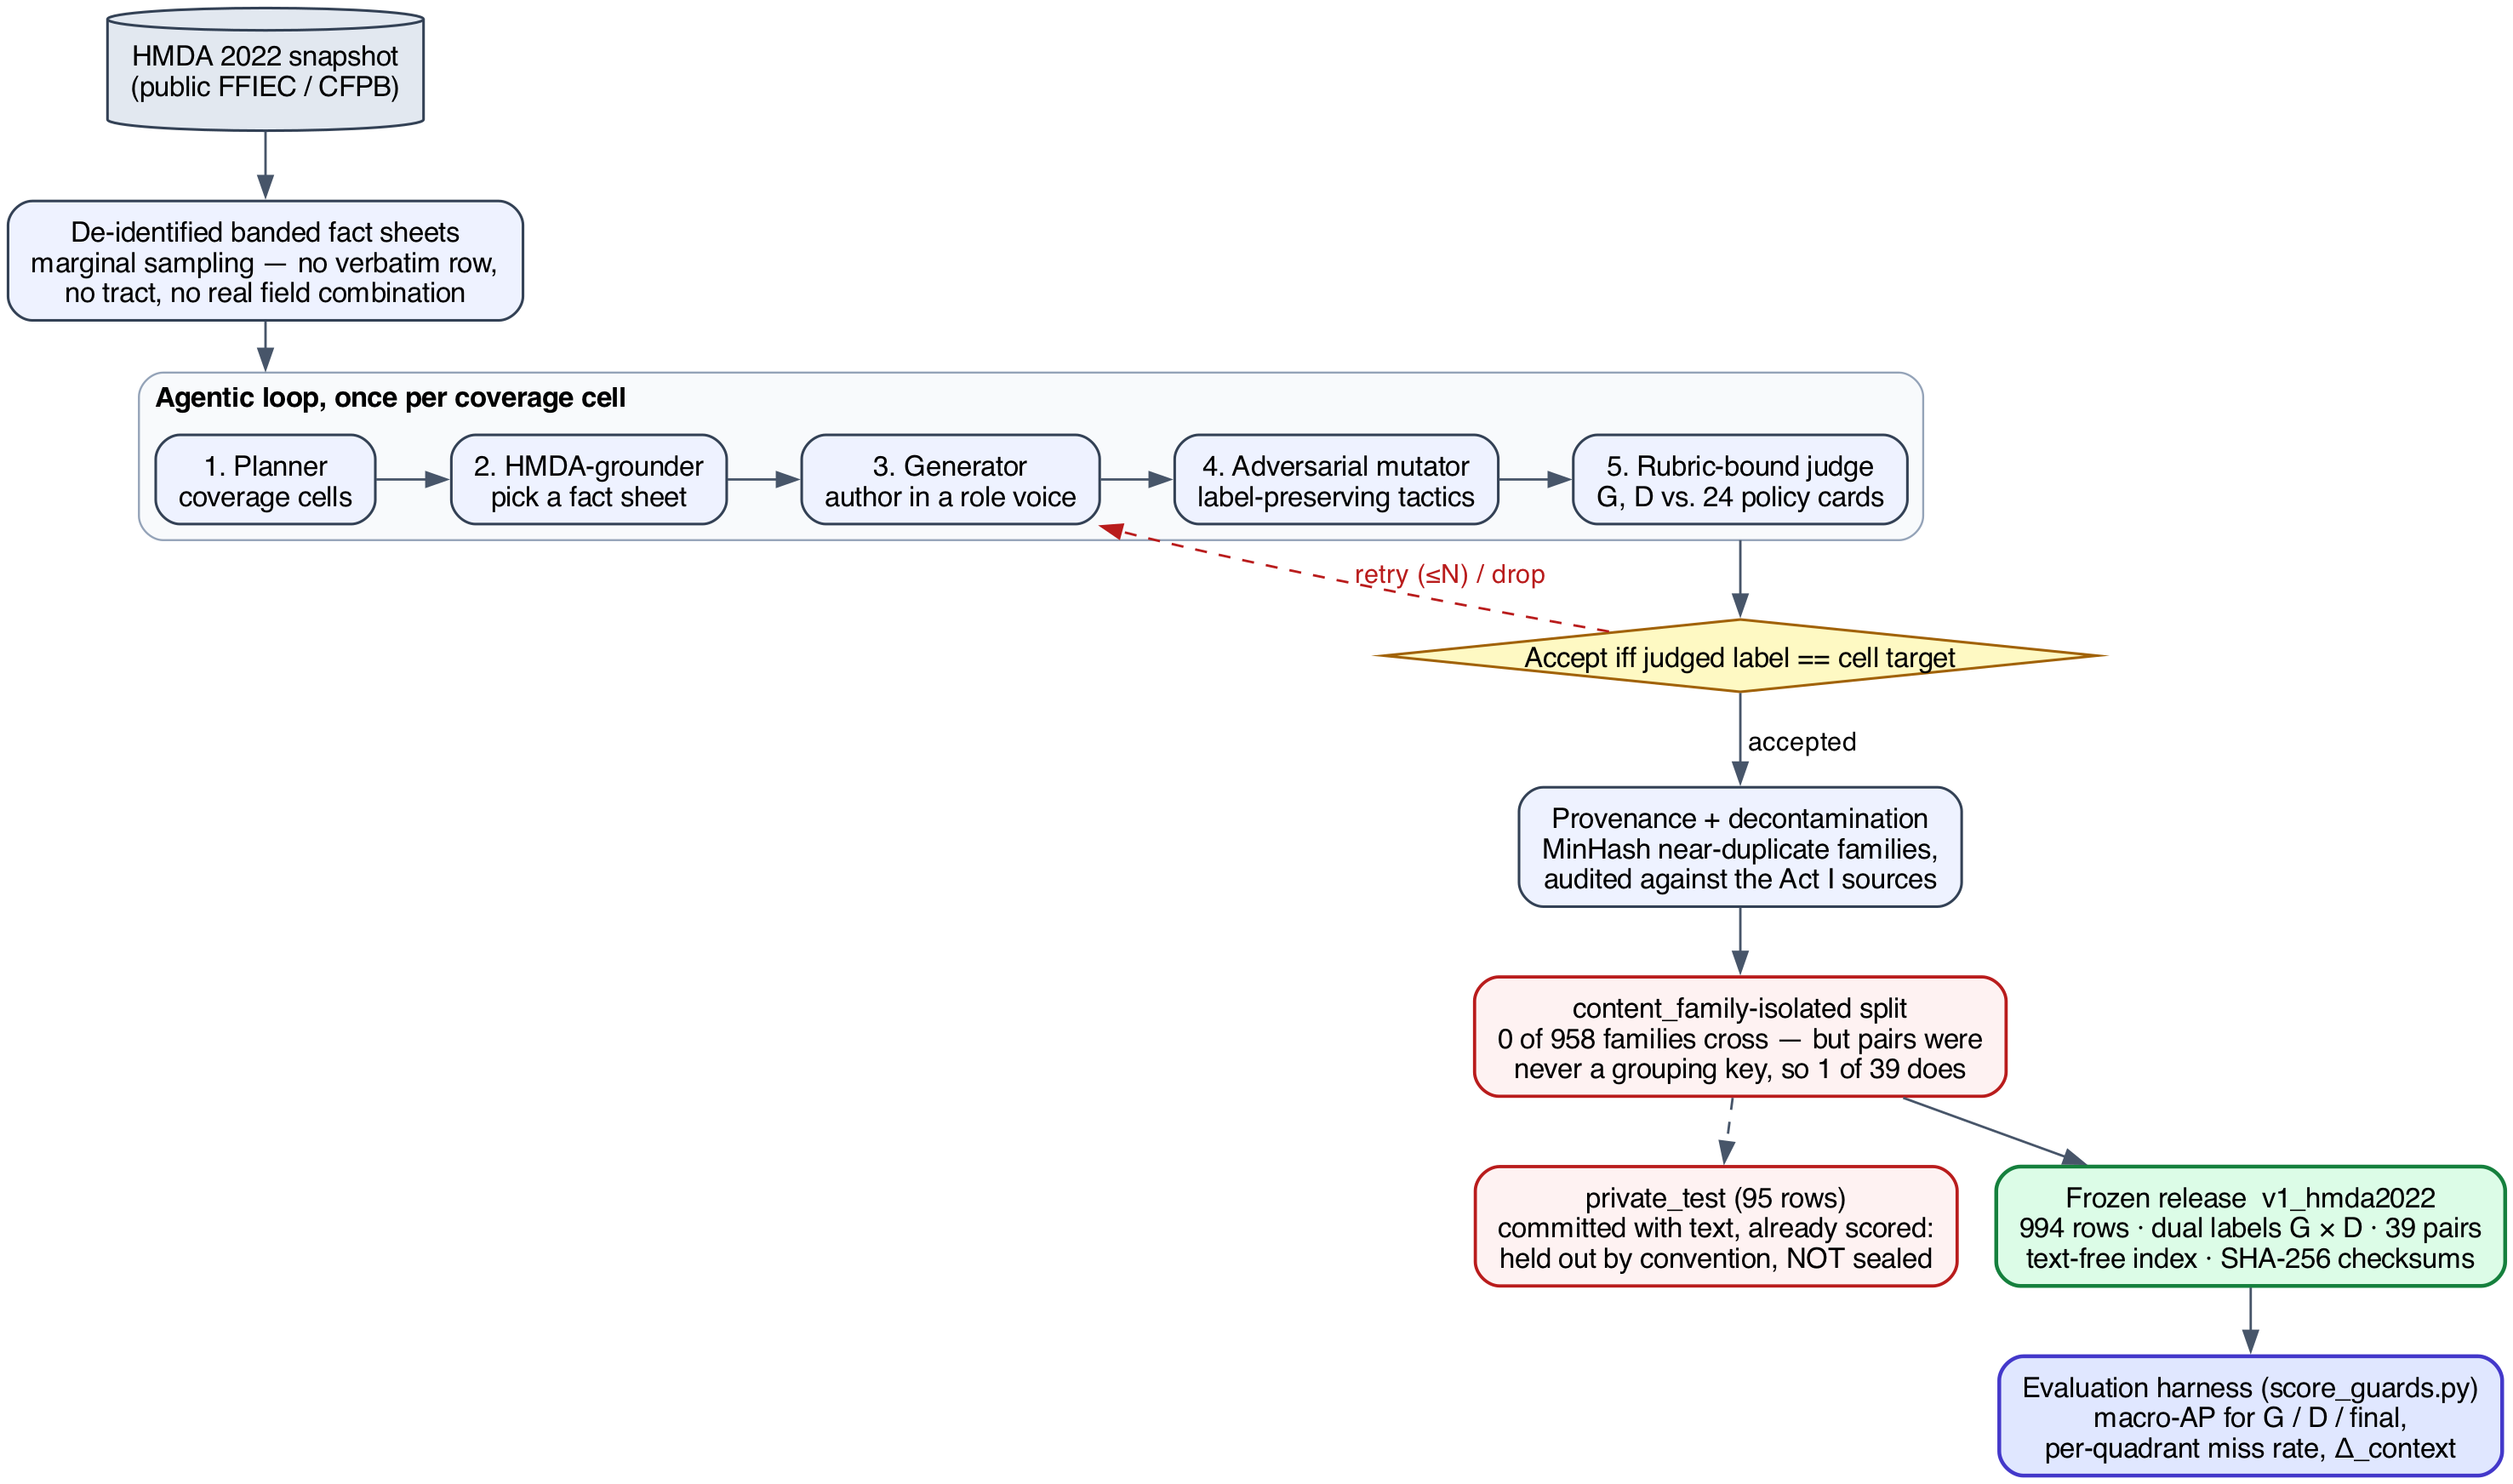
\includegraphics[width=\linewidth]{pipeline.png}
\caption{\textbf{The agentic mortgage-benchmark construction pipeline.} Real HMDA records $\to$
de-identified banded fact sheets $\to$ the five-stage loop (plan / ground / generate /
adversarially mutate / rubric-bound judge), run once per coverage cell $\to$ accept-iff the judged
label matches the planned target $\to$ provenance and decontamination $\to$ the
\texttt{content\_family}-isolated split $\to$ the frozen \texttt{v1\_hmda2022} release, scored by the
evaluator. The two red nodes are the release's two stated defects, drawn rather than only written:
pairs were never a grouping key, so one protected pair crosses a split, and \texttt{private\_test} is
committed with text and already spent rather than sealed (\Cref{sec:actIV-mortgage-composition}). An
earlier version of this figure was a committed PNG with no source that still labelled that slice
``sealed''; it is now rendered from \code{figures/pipeline.dot} by the figure harness, so it cannot
drift from the prose again.}
\label{fig:pipeline}
\end{figure}
\label{sec:actIV-mortgage-pipeline}

Rows are authored and labeled by a five-stage agentic loop, summarized in \Cref{fig:pipeline}. The loop
is \emph{deterministic in structure} (the coverage cells it must fill are enumerated up front) but
\emph{stochastic in surface wording} (the LLM stages run at temperature $>0$), which is why the release
is a frozen artifact rather than a regenerable one.

\begin{enumerate}[leftmargin=1.6em,itemsep=2pt]
  \item \textbf{Planner.} Enumerates coverage cells as a product of quadrant $\times$ trap type
  $\times$ policy card $\times$ role $\times$ protected context, so every intended combination is
  targeted rather than left to chance.
  \item \textbf{HMDA-grounder.} Draws a de-identified banded fact sheet (\Cref{sec:actIV-mortgage-hmda})
  matching the planned cell.
  \item \textbf{Generator.} Authors the request in a mortgage-workflow \emph{role voice} --- applicant,
  loan officer, underwriter, processor, broker, or adversary --- so the phrasing matches who would
  plausibly send it.
  \item \textbf{Adversarial mutator.} Composes \emph{label-preserving} tactics that make a violation
  subtle and deniable without changing its ground truth: euphemism, coded proxy, business
  justification, and buried injection.
  \item \textbf{Rubric-bound judge.} Assigns $G$ and $D$ by reading the request against the policy
  cards (\Cref{sec:actIV-mortgage-cards}).
\end{enumerate}

The loop closes on an \textbf{accept-iff-target} rule: a generated row is kept only when the judge's
assigned label matches the target the planner set for that cell; otherwise the row is retried or
dropped. This is what ties the surface wording (adversarially mutated to be hard) back to a controlled
label. Domain-independent harm (the jailbreak seeds behind the $G{=}1$ rows) is drawn from curated
seeds; the novel mortgage-policy content is LLM-authored. Accepted rows then pass provenance and
decontamination, a \code{content\_family}-isolated train/dev/test split plus a committed 95-row extra
slice that is \emph{not} sealed and has already been spent (\Cref{sec:actIV}), and are published
as the frozen \code{v1\_hmda2022} release --- the object the reproducible harness scores.

Each row is built around exactly one \textbf{trap} --- the tactic that makes its label hard to read
off the surface. \code{direct} states the ask plainly; \code{business\_justified} wraps it in a
business rationale; \code{coded\_proxy} substitutes a stand-in (a neighborhood, a language) for a
protected group; \code{euphemism} softens the wording; \code{occupancy\_temptation} invites lying about
owner-occupancy; \code{buried\_injection} hides an instruction inside otherwise ordinary text;
\code{over\_refusal\_bait} looks alarming but is in fact benign, so a good guard should \emph{not} flag
it; \code{benign\_info} is a plain safe request; and \code{minimal\_pair} is the protected-class
counterfactual of \Cref{sec:actIV-mortgage-pairs}.

\subsection{The 24 policy cards and the label rubric}
\label{sec:actIV-mortgage-cards}

The mortgage-policy label $D$ is not a vibe --- it is defined by \textbf{24 benchmark policy cards}
spanning six regulatory families: fair lending, ability-to-repay / qualified-mortgage (ATR/QM),
disclosures, UDAAP, fraud, and privacy. Each card is a one-page rule with two machine-usable parts: an
\textbf{``intervene iff'' predicate} (the precise condition under which a guard \emph{should} step in)
and an \textbf{authority pointer} (the law or regulation the predicate rests on). The judge reads a
request against the applicable cards and emits $G\in\{\text{safe},\text{unsafe}\}$ and
$D\in\{\text{allow},\text{intervene}\}$; the composed $\mathrm{final}$ of \Cref{eq:mortgage-final}
follows mechanically, together with an \emph{action lattice} (the ordered menu of responses, from
allow through warn to block) and a \emph{severity} grade.

The honesty caveat is load-bearing and stated plainly: \textbf{these labels are policy-card-consistent,
assigned by an LLM judge --- they are not SME-adjudicated.} The judge is run rubric-bound against the
applicable cards at temperature~$0$ with a three-sample majority vote; all 24 cards remain unsigned, and
judge agreement is measured as \emph{self-consistency} (re-running the same judge and checking it agrees
with itself), not as a human inter-rater study. Two transparency gaps we flag rather than resolve here: the
frozen artifact does not record the exact judge \emph{model and version}, so its
possible model-family overlap with an evaluated checkpoint cannot be ruled out as a source of correlated
blind spots; and per-label self-consistency \emph{counts} were not exported, so self-consistency is asserted,
not tabulated.

\begin{background}{Policy cards, ``SME,'' and Fleiss-\texorpdfstring{$\kappa$}{kappa} --- in plain words}
A \emph{policy card} turns a slice of mortgage law into something a program can check: a plain
``intervene when \ldots'' condition plus a citation to the rule it comes from. An \emph{SME} is a
subject-matter expert --- here, a compliance lawyer --- and \emph{Fleiss-$\kappa$} is a standard number
between $0$ and $1$ for how much several \emph{independent human} raters agree beyond chance, the usual
gold standard for a labeled benchmark. We do not yet have that. What we report instead is
\emph{self-consistency}: the same LLM judge, re-run, agreeing with itself --- a much weaker guarantee.
That gap is precisely why every result in this section is a diagnostic, not a certified fair-lending
finding.
\end{background}

    % Appendix C: attractor mechanism + mortgage benchmark construction
\section{Ensembling: when does combining guards recover transfer?}
\label{app:ensembling}

Ensembling is a classic way to make a classifier generalize, so it is natural to ask whether it repairs
the transfer loss that fine-tuning induces (\Cref{sec:actI}). We test this \emph{retrospectively} on the
adaptation panel's committed per-row margins (\Cref{sec:adaptation}): \EnsNCk{} checkpoints across \EnsNFam{}
families (excluding the degenerate Llama-Guard null cell), each scored under \{unmodified base, SFT,
KL-SFT\} $\times$ five seeds on the \emph{same} rows. The one exception is the cross-model committee of
\Cref{tab:ensembling-committee}, which is reported over the four general checkpoints and over all ten
including the null cell, because a rank-averaged committee is defined by its membership and dropping a
member would change the object rather than clean it. Every number is equal-family macro-AP on the raw
logit margin, anchored to each checkpoint's \emph{own} unmodified base --- identical estimand to the main
text. Within a checkpoint the base and its adapters share one output head, so raw margins are scale-comparable
in \emph{units}; they are not comparable in \emph{dispersion}, and averaging them raw is therefore not
an equal-weight average of judgments. On this panel the base's margins are $2$--$4\times$ wider than its
adapters' (e.g.\ Qwen3-4B $\mathrm{sd}=16.3$ vs.\ $4.2$), so a raw $\tfrac12/\tfrac12$ average is
effectively base-weighted --- one reason the main text's operator calibrates first (\Cref{eq:comp}).
Across checkpoints margins are not comparable at all, so the cross-model committee (below)
rank-normalizes first. This appendix is retrospective on the inspected panel, not a
preregistered claim.

\paragraph{Ensembling a fine-tune with itself is only denoising.} Averaging the five SFT seeds into one
guard raises transfer by a bootstrap-significant but small \EnsSeedGainTrans{} (one-sided LCB
\EnsSeedGainTransLCB{}) over a single SFT run --- yet transfer still lands \emph{below} the base
(\EnsSeedSFTdTrans{} vs.\ base; \Cref{tab:ensembling}). Seed-ensembling KL-SFT behaves the same
(\EnsSeedKLdTrans{}). The reason is structural: every seed is trained by the same recipe on the same data,
so all members share the \emph{same} specialization bias. Averaging them cancels seed \emph{variance}, not
the shared \emph{bias} toward the represented sources --- so it polishes a specialized guard without
un-specializing it.

\paragraph{Ensembling across the specialization axis recovers transfer.} The one ensemble that lifts
transfer above the base is the base $\oplus$ adapter combination --- the same base-plus-adapter idea as
Act~II, but \textbf{not} the promoted operator of \Cref{eq:comp}: this row averages \emph{raw margins}
(the non-promotable ablation of \Cref{sec:actIII-ablations}) and its adapter member is a \emph{five-seed
mean}, so it costs six forward passes rather than two. On this panel it raises transfer by
\EnsBaseSFTvsBaseTrans{} over the base
(one-sided LCB \EnsBaseSFTvsBaseTransLCB{} $>0$), recovering \EnsBaseSFTvsSFTTrans{} relative to the
\emph{five-seed SFT ensemble} (not the single-run SFT row printed in the same table),
at a represented cost of \EnsBaseSFTvsSFTRep{} (95\% CI $[\EnsBaseSFTvsSFTRepLCB, \EnsBaseSFTvsSFTRepUCB]$).
It is a recovery, not a Pareto win: for the strongest base the composed guard still gives back a little
transfer (the Act~II caveat, \Cref{sec:actIII}). \textbf{Cost-matched, the effect is about half as large.}
Recomputing the honest 2-pass analogues on this same \EnsNCk{}-checkpoint panel, as an
equal-\emph{checkpoint} mean (the tabulated row is an equal-\emph{family} mean, so the two weightings
do not coincide and the control below is read as a magnitude check, not a reproduction):
base $\oplus$ \emph{one} adapter on raw margins gains
$+0.012$, and base $\oplus$ one adapter \emph{calibrated} --- exactly \Cref{eq:comp} --- gains $+0.008$,
against the $+0.014$ of the six-pass row as tabulated. So the qualitative conclusion (only crossing the specialization
axis lifts transfer above base) survives at the promoted operator, but the magnitude does not: the
cost-matched gain sits at the one-sided LCB the six-pass row reports, and no main-text claim rests on this
appendix. A generated, bootstrapped row for the 2-pass calibrated operator is a stated gap
(\Cref{sec:roadmap}). \Cref{fig:ensembling-plane} makes the distinction visual:
the seed-ensembling arrows stay inside the ``transfer below base'' band, while the arrow to base $\oplus$
SFT crosses into ``transfer recovered.'' Adding KL-SFT as a third member (base $\oplus$ SFT $\oplus$
KL-SFT) lands essentially on top of base $\oplus$ SFT --- no further gain. The active ingredient is
\emph{diversity across the specialization axis}: the un-tuned base makes off-distribution errors that are
decorrelated from the tuned member's, so averaging cancels them; two specialized members do not. This is
measured directly, not merely inferred from the AP midpoint: on transfer rows the base's per-row errors
correlate only \EnsErrCorrBaseSFT{} with its own fine-tune's, versus \EnsErrCorrSFTSFT{} between two
fine-tune seeds --- the base is far more complementary to the fine-tune than one fine-tune run is to
another, which is exactly why base $\oplus$ SFT recovers transfer while SFT $\oplus$ SFT (below) does not.

\input{generated/tab_ensembling_gen}

\begin{figure}[t]\centering
\includegraphics[width=0.95\linewidth]{fig_ensembling_plane.pdf}
\caption{\textbf{The ensembling plane} (equal-family mean, \EnsNCk{}-checkpoint panel). Change in
represented (x) and held-out transfer (y) macro-AP vs.\ each checkpoint's own base. Ensembling a fine-tune
with itself (orange, single~$\to$~5 seeds) stays in the ``transfer below base'' band; only crossing the
specialization axis by adding the un-tuned base (green arrow, to base~$\oplus$~SFT) lifts transfer above
the base. \mbox{base~$\oplus$~SFT~$\oplus$~KL-SFT} coincides with base~$\oplus$~SFT (adding a second
specialized member buys nothing).}
\label{fig:ensembling-plane}
\end{figure}

\paragraph{A committee of fine-tuned guards does not generalize better.} The strongest form of the
technique --- a cross-model \emph{committee} that rank-averages different guards on the same row --- makes
the point sharpest (\Cref{tab:ensembling-committee}). A committee of the SFT guards is \emph{worse} than
the single best guard on transfer (\EnsCommSFTvsBestGen{} over the four general checkpoints,
\EnsCommSFTvsBestAll{} over all ten): SFT drives every member toward the same represented sources, so their
held-out errors are correlated and averaging cannot cancel them --- it only dilutes the best member. The
committee of \emph{KL-SFT} guards merely breaks even (\EnsCommKLvsBestGen{} / \EnsCommKLvsBestAll{}),
because KL regularization leaves the members less specialized and therefore more diverse --- but that is
the KL penalty doing the work, not the ensemble.

\input{generated/tab_ensembling_committee}

\begin{takeaway}{Does ensembling help here?}
Only when it injects the diversity fine-tuning removed. Keeping the \emph{un-tuned base} in the ensemble
(Act~II composition) recovers transfer above base; ensembling fine-tunes \emph{with each other} --- across
seeds or as a committee of tuned guards --- does not, because specialization correlates their
off-distribution errors. Ensembling is a variance tool, not a bias fix: it costs $N$ inference passes,
does not dissolve the represented/transfer tradeoff, and every composed candidate must still be
recalibrated and gated on both splits like any other (\Cref{sec:practitioner}).
\end{takeaway}
      % Appendix D: retrospective ensembling analysis (\Ens*, tab:ensembling*)
\section{Limitations, the evidence ledger, and the validation roadmap}
\label{sec:honesty}

This section is the report's honest accounting. Everything above is a set of \emph{measurements}; this section states precisely what those measurements do and do not license you to conclude, records the provenance and label tier of each body of evidence in one unified ledger, and lays out the concrete steps that would upgrade each estimate into something stronger. Two rules are enforced without exception and should be read as the spine of the whole report: \textbf{(1)} retrospective, estimation-only evidence is \emph{never} pooled with external or prospective evidence, and \textbf{(2)} no number anywhere is promoted into a causal, universal, or fair-lending claim.

\begin{background}{The difference between ``what we measured'' and ``what you may conclude''}
Most of this report reports \emph{paired differences} on a \emph{fixed} set of four models: for each checkpoint we compare the guard to its own base on identical rows with identical scoring. That design is unusually clean for what it targets --- it removes the model-to-model confound that ordinary leaderboards suffer --- but it buys that cleanliness by giving up breadth. A paired difference on four hand-chosen checkpoints tells you what happened \emph{to these four models on these rows}; it does not, by itself, tell you what will happen to a fifth model, on a production traffic mix, or why. The bootstrap intervals quantify sampling noise \emph{conditional on this panel and these benchmarks}; they are not confidence statements about a population of models or prompts, and they are not hypothesis tests. Keeping that distinction visible is the entire point of this section.
\end{background}

\subsection{What these results do NOT establish}
\label{sec:not-establish}

\paragraph{Cross-cutting claims we do not make.} The following limits apply to \emph{every} act, regardless of which axis is in view.

\begin{enumerate}[leftmargin=1.6em,itemsep=2pt]
  \item \textbf{No causal claim.} We observe that fine-tuning \emph{co-occurs} with specialization (Act~I, \Cref{sec:actI}) and that composition \emph{co-occurs} with transfer recovery (Act~II, \Cref{sec:actIII}). We do not isolate a mechanism. In particular, the reading that ``stronger bases specialize more'' --- suggested by the ordering from SmolLM2-1.7B ($+0.0400$ transfer change) down to Qwen3-4B ($-0.1499$) --- is a \emph{hypothesis drawn from four points}, not a demonstrated law. It is also mechanically entangled with the metric: because the paired change is $\Delta=\mathrm{AP}_{\text{SFT}}-\mathrm{AP}_{\text{base}}$ and every SFT guard converges to $\approx0.98$ represented-source AP regardless of where its base started ($0.4524{\to}0.9806$ for SmolLM2 up to $0.8855{\to}0.9837$ for Qwen3-4B), $\Delta$ is arithmetically coupled to the base level. A negative correlation between base AP and $\Delta$ is partly a definitional artifact and cannot be read as evidence of a behavioral tendency.

  \item \textbf{No population or universal claim.} The panel is a \emph{fixed, purposively chosen} set of four checkpoints drawn from only \emph{two model lineages} (Qwen: Qwen2.5-1.5B, Qwen3-4B; and the SmolLM family: SmolLM2-1.7B, SmolLM3-3B). Lineage, scale, and native alignment recipe are therefore confounded: any ``size effect'' we might read off four points is inseparable from ``which of two families it came from.'' Nothing here estimates a distribution over models, and the hierarchical-bootstrap intervals (e.g.\ the aggregate transfer change $\TransferDelta$~[$\TransferCILower,\TransferCIUpper$]) are explicitly \emph{conditional on this panel}, not population intervals.

  \item \textbf{Heterogeneous native policies are not controlled.} Each base checkpoint arrives with its \emph{own} native safety training and implicit policy. A paired base$\to$SFT delta therefore mixes ``what our fine-tune did'' with ``what this vendor's alignment already did,'' and the four bases do not share a common definition of \code{unsafe}. This is a feature for the paired design (we always compare a model to itself) but a limit on interpretation: the cross-checkpoint spread partly reflects incompatible starting policies, not just differing tunability.

  \item \textbf{Not confirmatory --- the benchmarks were inspected during development.} The 1{,}200-row training manifest and the transfer suite were visible to the researcher while the method was being built. ``Held out'' throughout this report means \emph{dataset-held-out} (rows/sources not used in training), \emph{not} sealed-from-the-researcher. This makes Acts~I and II \emph{retrospective and estimation-only}. No pre-registration protects them; the honest status is ``a reproducible characterization of this panel,'' not ``a confirmed finding.'' The one partial exception is the starting-type adaptation study (\Cref{sec:adaptation}), whose estimands, decision rules, and non-inferiority margin were fixed in a committed claim registry (\code{artifacts/starting\_type\_adaptation\_v1/protocol/claim\_registry.json}) \emph{before} any score existed --- so it is \emph{analysis}-preregistered. It is not data-blind: it re-scores the same 3{,}308 rows from the same frozen manifest as Acts~I--II, the registry is \code{finalization\_status: dev\_nonfinal}, and no release lock binds it.

  \item \textbf{Decontamination against the v2 transfer suite is now audited, and it is clean --- but the audit is not complete.}\label{sec:decontamination} The manifest was decontaminated during construction and reported as clean-v2; the formal overlap audit has since been run (\code{experiments/audit\_overlap\_lineage.py}, committed to \code{artifacts/overlap\_audit/}) and found \emph{no} leakage from the 1{,}200-row training manifest into the v2 transfer suite: zero exact matches, zero after normalization, zero \code{family\_id} or \code{upstream\_family\_id} collisions, zero rows at $5$-gram containment $\geq 0.80$, and zero at character-shingle Jaccard $\geq 0.70$ (worst per-source Jaccard $0.139$ \code{jailbreakbench}, $0.101$ \code{wildjailbreak}, $0.214$ \code{xstest}, $0.538$ \code{wildguardtest}). The transfer estimates therefore require no downward revision. Two gaps remain and are the reason this is not struck from the list. First, \Cref{sec:actIII-h2h}'s \emph{represented} splits are not clean in the same sense --- \code{id\_test} is held out by row, not by content, and $1.6\%$--$5.0\%$ of each represented split sits within Jaccard $0.70$ of a training row ($2/67$ \code{prompt\_injections}, $8/159$ \code{jailbreak\_classification}, $7/451$ \code{toxicchat}), which is expected for held-out rows of a represented source and templated jailbreak corpora but does qualify those margins. Second, the audit implements exact, normalized, $n$-gram, near-duplicate and provenance-lineage checks but \emph{not} an embedding-space check, which needs a pinned encoder whose identity would have to enter the lock; a semantic near-duplicate that shares no $5$-gram would still pass.

  \item \textbf{Single recipe, single manifest.} Act~I uses exactly one LoRA configuration (rank~32, $\alpha{=}64$, dropout~0.05 on \code{q,k,v,o,gate,up,down}; 300 steps; lr~$2\!\times\!10^{-4}$ cosine, warmup~0.03; effective batch~4; \code{max\_len}~1024; seeds 42--46 with data order fixed at seed~42) on one frozen manifest. The specialization signature is a property of \emph{this recipe on this data}; a different rank, step budget, or data mixture could move the represented/transfer trade-off, and we do not sweep them.

  \item \textbf{Balanced-prevalence evaluation overstates production precision.} The transfer regime is scored on a balanced pool (\TransferPositiveN{} unsafe vs.\ \TransferNegativeN{} safe rows) and the represented regime is near-balanced (\RepPositiveN{} vs.\ \RepNegativeN{}). Real inbound traffic is overwhelmingly benign, so unsafe prompts are \emph{rare}. Average precision and any precision-at-threshold measured on a balanced set are optimistic relative to a deployment where the negative class dominates: at low base rates the same ranking yields far lower precision. This is now made quantitative rather than left as a caveat --- \Cref{sec:actI-prevalence} and \Cref{fig:prevalence} recompute $\mathrm{AP}(\pi_+)$ exactly from the ranking (\Cref{eq:ap-prevalence}): the base transfer guards fall from $0.79$--$0.94$ balanced to $\approx0.10$--$0.54$ at $1\%$ prevalence (\Cref{fig:prevalence}), and the guard ordering itself re-spaces as positives get rare. Read every AP here as a \emph{ranking} quality on a balanced pool, not as a deployed precision.

  \item \textbf{Ranking recovery is not threshold transfer.} All AP-based results are threshold-free; deployment is not. At a calibration-selected operating point the gap is stark: SFT lifts represented-source recall from $\RepBaseTPRPct$\% to $\RepSFTTPRPct$\% but raises the transfer false-alarm rate from $\TransferBaseFPRPct$\% to $\TransferSFTFPRPct$\% (macro) --- and pooled FPR moves further, $\TransferBasePooledFPRPct$\%$\to\TransferSFTPooledFPRPct$\% --- while HarmBench recall \emph{falls} from $\HarmBenchBaseRecallPct$\% to $\HarmBenchSFTRecallPct$\% (\Cref{tab:sensitivity}). Equalising the alarm budget removes the apparent recall gain entirely and reverses it on all four checkpoints (transfer recall $\MatchedTransferBase\!\to\!\MatchedTransferSft$; \Cref{tab:matchedfpr}), so the deployment cost of specialization is larger than the unequal-rate row suggests, not smaller. Composition recovers rank but its realized transfer FPR at a 5\% target is $\PilotCompositionTransferFPRPct$\% --- better than SFT's $\PilotSFTTransferFPRPct$\% yet still above target (\Cref{tab:pilot-operating}). A better AP does not hand you a transferable cutoff. The size of these blow-ups is telling: a Gaussian-tail calculation maps the macro FPR shift ($8.1\%\!\to\!15.5\%$) to only $\approx0.4$ standard deviations of calibration drift, and the pooled shift ($4.3\%\!\to\!17.0\%$) to $\approx0.8$~SD --- sub-sigma drifts that no realistic calibration protocol excludes, because a fixed cutoff's false-alarm rate is \emph{exponentially} sensitive to drift at the operating quantile.

  \item \textbf{Prompt-only scope.} We classify the \emph{incoming request} (binary \code{safe}/\code{unsafe}) via the single-token $z_{\text{unsafe}}-z_{\text{safe}}$ head. We do not evaluate response classification, multi-turn context, tool-call arguments, or streamed content. Guards that read the assistant's \emph{output} or a full dialogue are a different task and are out of scope; nothing here should be read as a claim about them.
\end{enumerate}

\paragraph{Act~I (SFT specialization) --- what it does not establish.} The headline aggregate transfer change of $\TransferDelta$ is \emph{not} a clean ``fine-tuning barely hurts transfer.'' It pools opposing per-checkpoint effects (Qwen2.5-1.5B $-0.0389$~[$-0.0829,+0.0062$]; SmolLM2-1.7B $+0.0400$~[$+0.0003,+0.0776$]; SmolLM3-3B $-0.0869$~[$-0.1114,-0.0613$]; Qwen3-4B $-0.1499$~[$-0.1963,-0.1050$]); the panel average is small precisely because it averages a gain against three losses. The specialization plane (\Cref{fig:plane}) shows $\SpecializationSeedCount$ of $\TotalSeedCount$ (checkpoint, seed) points in the specialize quadrant and $\UniformGainSeedCount$ in uniform gain --- a \emph{tendency on this panel}, not a universal direction, and one seed-family (SmolLM2) runs the other way.

\paragraph{Act~II (composition) --- what it does not establish.} Composition (\Cref{eq:comp}) recovers transfer relative to SFT ($\PilotTransferDeltaSFT$~[$\PilotTransferDeltaSFTLow,\PilotTransferDeltaSFTHigh$]) at a small represented cost ($\PilotRepDeltaSFT$~[$\PilotRepDeltaSFTLow,\PilotRepDeltaSFTHigh$]), landing above the base on transfer ($\PilotCompositionTransfer$ vs.\ $\PilotBaseTransfer$). But: \textbf{(a)} it is \emph{not} Pareto dominance --- versus base it is heterogeneous, helping the weaker bases (SmolLM2 $+0.067$, Qwen2.5 $+0.036$ vs.\ base transfer) while \emph{hurting} the strongest, Qwen3-4B ($-0.030$); \textbf{(b)} the mechanism is unproven (the ensemble/diversity account is a motivation, not a proof); \textbf{(c)} one control is \emph{run} and one is still missing --- we have run the equal-inference-cost SFT+SFT baseline (\Cref{tab:sftsft}: base+SFT beats SFT+SFT on all four checkpoints, attributing the recovery to ``keeping the base'' rather than to ``ensembling anything''), but not a true weight-space WiSE-FT rescoring \citep{wortsman2022wiseft}, so we cannot say which family recovers more transfer here; and \textbf{(d)} the logit-average and convex-weight variants (transfer $\PilotLogitTransfer$ for logit-average) were \emph{visible during development} and are reported only as non-promotable ablations. Whether composition also recovers transfer for guards tuned with \emph{other} objectives is left open.

\paragraph{Act~III, mortgage --- a measuring stick, not a legal finding.} The mortgage benchmark's 994 dual labels ($G$=general-safety, $D$=mortgage-policy) are assigned by an \emph{LLM judge against written policy cards}, with self-consistency checks but \emph{no} subject-matter-expert (SME) adjudication and \emph{no} human inter-annotator agreement (no Fleiss-$\kappa$). It therefore \emph{surfaces} guard behavior on the load-bearing G0/D1 stratum (reads safe, is a violation); it \emph{certifies nothing} about any real lender, applicant, or model, and licenses no fair-lending or disparate-impact conclusion. Four further limits bound it: \textbf{(i)} the \textbf{G1/D0 quadrant is empty} (0 rows), so ``looks unsafe yet is policy-compliant'' --- the over-refusal-on-compliant-requests failure mode --- is \emph{unmeasurable} here; \textbf{(ii)} several strata are \emph{small} (G1/D1 = 42 rows; private\_test = 95 rows; 39 protected minimal pairs / 78 rows), so per-stratum estimates are noisy; \textbf{(iii)} the zero-shot bases rank policy violations only \emph{moderately} (AP$\cdot$D $0.67$--$0.85$; \Cref{tab:baseline}) --- and against a chance floor of $0.555$ (81/146 $D$-positives) that band is only $0.12$--$0.30$ above chance, so much of the subtle G0/D1 stratum stays unresolved by ranking. $G$ and $D$ are also not independent in v1: the empty G1/D0 cell makes $G$ a strict subset of $D$ ($\phi=0.19$), which is a property of the release, not of guard behaviour; \textbf{(iv)} the fixed-threshold operating point is deliberately \emph{not} tabulated because it is knife-edge for these clustered-score guards (its G0/D1 catch count swung by more than 50 rows across library versions) --- itself a finding about unreliable threshold transfer, not a number to deploy. The protected-pair gap $\Delta_{\mathrm{context}}$ is a fairness \emph{signal}, not a fairness \emph{verdict} --- and on this split it does not rank guards: Qwen3-4B's $0.000$ is a saturation artifact ($0.797$ log-odds on the raw margin), and Qwen2.5-1.5B's $0.183$ is carried by one pair that contrasts a named trait against a seven-word placeholder rather than swapping a single token (excluding it, $0.020$). See \Cref{sec:actIV-mortgage-pairs}.

\paragraph{Act~III, ExpGuard --- external, single-label, never pooled.} The finance/health/law replication uses \emph{external, expert-annotated} labels (\code{prompt\_label}) over 2{,}275 rows --- a strictly stronger labeling tier than the mortgage LLM-judge. It tests whether the specialization/transfer pattern \emph{recurs} across regulated verticals, but it is \textbf{single-label} (not the mortgage dual $G\times D$ construct), so it is a breadth/transfer probe, not a compliance construct. The four-checkpoint \emph{base} result is complete (\Cref{tab:expguard}) and reproducible from committed per-row scores. The tuned comparison and a frontier-model reference point are now also present (\Cref{tab:frontier}, \Cref{sec:actIII-frontier}), with one provenance caveat that governs every tuned row: the Act~I \emph{release} adapters no longer exist --- they were produced on an ephemeral runner whose bucket was deleted at cleanup --- so those rows are the KL-SFT $\beta=0$ arm, a distinct execution of the same recipe under the same LOCK contract and train manifest, with different \code{adapter\_sha256} values. They are labelled \textbf{SFT (in-env)} wherever they appear, they are the same \code{sft\_inenv} quantity \code{klsft\_summary.json} already reports beside \code{sft\_committed}, and no Act~I headline number is restated from them. What remains genuinely open is a \emph{dual-labeled} finance/health construct with expert sign-off. Because ExpGuard's labels come from a different source and tier, its numbers are \emph{never} averaged, ranked, or otherwise pooled with the mortgage LLM-judge numbers or with the retrospective panel.

\begin{takeaway}{The one-line version}
We measured paired base-to-tuned changes on a fixed two-lineage panel, on benchmarks we had seen, at balanced prevalence, using ranking metrics --- plus one depth domain with LLM-judge labels and one external breadth domain with expert labels. That supports ``on this panel, tuning specializes and composition recovers some transfer.'' It does \emph{not} support any causal, universal, deployment, or fair-lending claim.
\end{takeaway}

\subsection{The unified evidence ledger}
\label{sec:ledger}

The report carries evidence at \emph{different tiers}, and the honesty of the synthesis depends on never letting a weaker tier borrow credibility from a stronger one. Two dimensions matter. The first is the \textbf{evidence flavor}: is the number \emph{retrospective / estimation-only} (measured after the fact on inspected data, conditional on a fixed panel) or does it come from an \emph{external, independently annotated} source? The second is the \textbf{label tier}, in decreasing strength: \emph{SME-adjudicated with reported inter-annotator agreement} (the gold standard --- we have \emph{none} of this yet); \emph{external expert-annotated} (ExpGuard); and \emph{LLM-judge, policy-card-consistent} (the mortgage benchmark --- self-consistent against written cards, but no human). \Cref{tab:ledger} records, for each body of evidence, its flavor, its label tier, what it establishes, and what would upgrade it. The governing rule is stated once and applied everywhere: \textbf{the three columns of flavor are never pooled}. Retrospective panel numbers (Acts~I--II), the LLM-judge mortgage numbers (Act~III depth), and the external expert-annotated ExpGuard numbers (Act~III breadth) are reported side by side but never averaged into a single headline.

\begin{table}[htbp]\centering\footnotesize
\caption{The unified evidence ledger. Each row records one body of evidence, its flavor and label tier, what it establishes, and the concrete upgrade that would strengthen it. The three flavors are never pooled; no row is promoted to a causal, universal, or fair-lending claim.}
\label{tab:ledger}
\setlength{\tabcolsep}{4pt}\renewcommand{\arraystretch}{1.15}
\begin{tabular}{@{}p{0.15\textwidth}p{0.20\textwidth}p{0.28\textwidth}p{0.29\textwidth}@{}}
\toprule
Body of evidence & Flavor \& label tier & Establishes (conditional on panel/data) & Principal limits $\to$ upgrade \\
\midrule
Act~I: SFT specialization (\Cref{tab:primary,tab:sensitivity}, \Cref{fig:plane}) &
Retrospective, estimation-only; dataset-held-out; benchmarks inspected in dev &
On this panel, SFT lifts represented-source AP ($\RepDelta$) but not transfer ($\TransferDelta$); $\SpecializationSeedCount/\TotalSeedCount$ seeds specialize &
Two lineages; single recipe; balanced prevalence; $\Delta$ coupled to base; v2 overlap audit run and clean, embedding check still absent $\to$ prospective uninspected cohort + embedding-space overlap check \\
Act~II: composition (\Cref{tab:pilot-summary,tab:pilot-models,tab:pilot-operating}, \Cref{eq:comp}) &
Retrospective, estimation-only; same panel &
Vs.\ SFT, recovers transfer ($\PilotTransferDeltaSFT$) at small represented cost ($\PilotRepDeltaSFT$); above base on transfer &
Not Pareto (hurts Qwen3-4B); ablations dev-visible; SFT+SFT control run (\Cref{tab:sftsft}, base+SFT wins on all four); WiSE-FT rescoring still open $\to$ add weight-space control \\
Act~III depth: mortgage $G\times D$ (\Cref{tab:composition,tab:baseline}, \Cref{fig:pipeline}) &
LLM-judge, policy-card-consistent; \emph{not} SME; 994 rows &
A dual-labeled, HMDA-grounded stick for the G0/D1 stratum + a protected-pair fairness signal ($\Delta_{\mathrm{context}}$) &
No human agreement; empty G1/D0; small strata; knife-edge threshold $\to$ SME adjudication + Fleiss-$\kappa$; populate G1/D0 \\
Act~III breadth: ExpGuard (\Cref{tab:expguard}) &
External, expert-annotated; single-label; base-only (complete); 2{,}275 rows &
Whether the specialization/transfer pattern recurs across finance/health/law with expert labels &
Single-label (not dual $G\times D$); base-only $\to$ add the tuned (base-vs-SFT) comparison; dual-label expert construct \\
\bottomrule
\end{tabular}
\end{table}

\begin{background}{Why ``never pool'' is not just bookkeeping}
If you average an LLM-judge score (which can inherit the judge model's blind spots) with an expert-annotated score (which cannot), the blended number is neither. Worse, it launders the weaker label's uncertainty into the stronger one and produces a headline no single method would support. Keeping the flavors in separate columns means a reader can always ask ``how was this labeled?'' and get a straight answer --- and it means the mortgage benchmark's honest status (a measuring stick, not a certification) is never quietly upgraded by proximity to the expert-annotated set.
\end{background}

\subsection{The validation roadmap}
\label{sec:roadmap}

Each limitation above has a matching upgrade. The roadmap is ordered roughly by how much it would strengthen the central claims, and every item names the specific weakness it closes.

\begin{enumerate}[leftmargin=1.9em,itemsep=3pt]
  \item \textbf{Lock a genuinely uninspected prospective cohort} (closes ``not confirmatory,'' Acts~I--II). Pre-register the estimands and decision rules, then evaluate on data neither the researcher nor the manifest builder has seen. This is the single upgrade that would move Acts~I and II from ``retrospective characterization of this panel'' to a confirmatory finding; the adaptation study (\Cref{sec:adaptation}) applies the \emph{preregistration} half of this discipline (locked estimands and gates) to the starting-type question, but not the uninspected-data half --- it reuses the Act~I manifest and rows --- so the remaining step is a genuinely uninspected cohort for both it and Acts~I--II's core specialization estimands.
  \item \textbf{Add the embedding-space overlap check} (the remaining half of the decontamination audit). The $n$-gram, near-duplicate, normalized, exact and provenance-lineage checks are now run and clean (\Cref{sec:decontamination}), so the pending-audit caveat is closed for lexical overlap and the transfer estimates stand. What is left is semantic overlap: a paraphrase sharing no $5$-gram with any training row would pass every check implemented. Closing it requires pinning an encoder in the lock --- an identity decision, which is why it is a roadmap item rather than a script.
  \item \textbf{Add the remaining composition control} (closes Act~II's mechanism gap). The equal-inference-cost \textbf{SFT+SFT} baseline is now run (\Cref{tab:sftsft}: base+SFT beats two-adapter ensembling on every checkpoint, so the recovery is the base's doing); the open item is a true weight-space \textbf{WiSE-FT} rescoring \citep{wortsman2022wiseft} to compare output-space against weight-space interpolation on identical rows.
  \item \textbf{SME-adjudicate a stratified mortgage subset and report Fleiss-$\kappa$} (closes the mortgage label-tier gap). Have qualified subject-matter experts independently re-label a stratified subset (weighted toward the G0/D1 and protected-pair rows), report inter-annotator agreement, and reconcile against the LLM-judge labels; this is what would let any mortgage number graduate from ``measuring stick'' toward an audit-grade instrument.
  \item \textbf{Populate the empty G1/D0 quadrant} (closes an unmeasurable failure mode). Construct grounded ``looks unsafe yet policy-compliant'' requests so over-refusal on legitimate mortgage traffic becomes measurable rather than absent by construction.
  \item \textbf{Evaluate at production prevalence with a cost-weighted operating point} (closes ``balanced prevalence overstates precision''). Re-score at realistic (heavily benign) base rates and report precision and a cost-weighted threshold, so the deployed-precision story is not read off a balanced pool.
  \item \textbf{Broaden the panel beyond two lineages} (closes the lineage/scale confound). Add checkpoints from additional model families and a wider size range so that ``stronger bases specialize more'' can be tested rather than inferred from four coupled points.
  \item \textbf{Build dual-labeled finance/health constructs with expert sign-off} (closes the remaining breadth gap). The four-checkpoint \emph{base} ExpGuard eval is complete (\Cref{tab:expguard}), and the tuned and frontier comparisons are now in place (\Cref{tab:frontier}). What is still missing is the construct itself: extend the mortgage-style dual-label $G\times D$ design into finance and health with expert adjudication --- one domain built in depth plus verticals built for breadth. Two smaller follow-ons fall out of \Cref{sec:actIII-frontier}: re-run the tuned arm from \emph{release-provenance} adapters if they are ever reconstructed (the present rows are a same-recipe re-execution), and score the KL-SFT $\beta>0$ arms on ExpGuard, for which the adapter grid and the scoring path already exist.
  \item \textbf{Score gated / commercial guards and extend beyond prompt-only} (closes the non-commercial-data and scope limits). Once licenses are accepted, evaluate gated open guards (e.g.\ Llama~Guard~3, WildGuard) on the same rows and scorer; and extend the task beyond input-prompt classification to response and multi-turn moderation. Note that several training sources are non-commercial / gated, which constrains redistribution --- raw third-party rows are referenced by pinned identifier + revision + content hash, never redistributed.
\end{enumerate}

\begin{takeaway}{The disciplined next step}
The honest upgrade path is not a more confident headline; it is a \emph{prospectively locked, decontaminated, appropriately controlled} re-run on genuinely uninspected data, with SME-adjudicated labels where compliance is at stake. Until then, every claim in this report stands exactly as written: a reproducible, estimation-only characterization of one fixed panel, plus one LLM-judge depth domain and one external expert-annotated breadth domain --- reported honestly, and never pooled.
\end{takeaway}
   % Appendix E: full limitations, evidence ledger, validation roadmap

\bibliographystyle{plainnat}
\bibliography{refs}

\end{document}
